%%
\documentclass[english, 12pt, a4paper, elec, utf8, a-1b, online]{aaltothesis}

\usepackage{amsfonts,amssymb,amsbsy,amsmath}
\usepackage[vlined, ruled, linesnumbered, commentsnumbered]{algorithm2e}
\usepackage{biblatex}
\usepackage{bm}
\usepackage{bbm}
\usepackage{calc} % To reset the counter in the document after title page
\usepackage{caption}
\usepackage[inline]{enumitem}
\usepackage{graphicx}
\usepackage{gensymb}
\usepackage{hyperref}
\usepackage{layouts}
\usepackage{longtable}
\usepackage{mathtools}
\usepackage{multirow}
\usepackage{outlines}
\usepackage{subcaption}
\numberwithin{equation}{section}
% \mathtoolsset{showonlyrefs}


\setlist[itemize]{itemsep=0.1ex, topsep=0.8ex}
\setlist[enumerate]{itemsep=0.1ex, topsep=0.8ex}


\addbibresource{references.bib}

\newcommand{\amax}{a_\text{max}}
\newcommand{\amin}{a_\text{min}}

\newcommand{\ploss}{P_\text{loss}}

\newcommand{\pref}{P_\text{ref}}
\newcommand{\lref}{L_\text{ref}}

\newcommand{\glow}{g_\text{low}}
\newcommand{\ghigh}{g_\text{high}}

\newcommand{\sno}{SN_0}

\newcommand{\varcv}{\sigma_\text{CV}^2}
\newcommand{\varca}{\sigma_\text{CA}^2}
\newcommand{\msp}{\mu}

\newcommand{\Ne}{N_\text{e}}

\renewcommand{\vec}[1]{\mathbf{#1}}
\renewcommand{\Vec}[1]{\boldsymbol{#1}}

\newcommand{\tr}[1]{\texttt{Tr}\left\{ #1 \right\}}
\newcommand{\Pest}{P_{t+1|t}^{(k)}}
\newcommand{\etal}{\textit{et al}.~}
\newcommand{\Epolicy}[1]{\mathrm{E}_\pi \left[ #1 \right]}
\newcommand{\Ss}{\mathcal{S}}
\newcommand{\As}{\mathcal{A}}
\newcommand{\Rs}{\mathcal{R}}
\newcommand{\Ps}{\mathcal{P}}
\newcommand{\Os}{\Omega}
\newcommand{\Op}{O}
\newcommand{\argmax}{\text{argmax}}
\newcommand{\egreedy}{$\epsilon$-greedy~}
\newcommand{\E}[1]{\mathbb{E}\left[ #1 \right]}
\newcommand{\inv}[1]{#1^{-1}}
\newcommand{\sqinv}[1]{#1^{-\frac{1}{2}}}
\renewcommand{\Pr}[1]{\text{Pr}\left\{ #1 \right\}}

\newcommand{\xprior}{\hat{\vec{x}}_{k|k-1}}
\newcommand{\xpost}{\hat{\vec{x}}_{k|k}}
\newcommand{\xlast}{\hat{\vec{x}}_{k-1|k-1}}

\newcommand{\priorecov}{\boldsymbol{\Sigma}_{k|k-1}}
\newcommand{\postecov}{\boldsymbol{\Sigma}_{k|k}}
\newcommand{\lastecov}{\boldsymbol{\Sigma}_{k-1|k-1}}
\newcommand{\ecov}{\boldsymbol{\Sigma}_k}

\newcommand{\prefitinnov}{\vec{y}_k}
\newcommand{\postfitinnov}{\Tilde{\vec{y}}_{k|k}}

\newcommand{\x}{\vec{x}_k}
\newcommand{\xnext}{\vec{x}_{k+1}}
\newcommand{\xhat}{\hat{\vec{x}}_k}

\newcommand{\z}{\vec{z}_k}
\newcommand{\znext}{\vec{z}_{k+1}}

\newcommand{\stmodel}{\vec{F}_k}
\newcommand{\cimodel}{\vec{B}_k}
\newcommand{\cinput}{\vec{u}_k}
\newcommand{\pnoise}{\vec{w}_k}
\newcommand{\omodel}{\vec{H}_k}

\newcommand{\onoise}{\vec{v}_k}
\newcommand{\ocov}{\vec{R}_k}
\newcommand{\pcov}{\vec{Q}_k}
\newcommand{\innocov}{\vec{S}_k}

\newcommand{\eye}{\vec{I}}
\newcommand{\gain}{\vec{K}_k}

\newcommand{\normal}[2]{\mathcal{N}\left(#1, #2 \right)}
\newcommand{\xnormal}[3]{\mathcal{N}\left(#1; #2, #3\right)}

\newcommand{\Pd}{P_\text{D}}
\newcommand{\Pfa}{P_\text{FA}}
\newcommand{\SNR}{\text{SNR}}
\newcommand{\SN}{\text{SN}_0}

\renewcommand{\exp}[1]{\text{exp}\left( #1 \right)}
\newcommand{\transpose}[1]{#1^\text{T}}
\newcommand{\rotmat}{\mathbf{T}}

\newcommand{\tmax}{t_\text{max}}
\newcommand{\tmin}{t_\text{min}}
\newcommand{\nmax}{n_\text{max}}
\newcommand{\muca}{\mu_{\text{CA}}}
\newcommand{\mucv}{\mu_{\text{CV}}}

\newcommand{\stprobs}{\vec{P}}

\newcommand{\modeprob}{\mu_k^i}
\newcommand{\lastmxprobs}{\mu^{j|i}_{k-1|k-1}}
\newcommand{\mxnorm}{ \Bar{c}_i }
\newcommand{\xmxinit}{\hat{\vec{x}}^{0i}_{k-1|k-1}}
\newcommand{\xmxinitcurr}{\hat{\vec{x}}^{0i}_{k|k}}
\newcommand{\ecovmxinit}{\bm{\Sigma}^{0i}_{k-1|k-1}}
\newcommand{\ecovmxinitcurr}{\bm{\Sigma}^{0i}_{k|k}}
\newcommand{\modexlast}{\hat{\vec{x}}^{j}_{k-1|k-1}}
\newcommand{\modexprior}{\hat{\vec{x}}^{i}_{k|k-1}}
\newcommand{\modecovlast}{\bm{\Sigma}^j_{k-1|k-1}}
\newcommand{\modecovprior}{\bm{\Sigma}^i_{k|k-1}}
\newcommand{\modeinnovcov}{\mathbf{S}^i_{k}}
\newcommand{\modemxcovlast}{\Tilde{\bm{\Sigma}}^{ij}_{k-1|k-1}}
\newcommand{\modexpost}{\hat{\vec{x}}^{i}_{k|k}}
\newcommand{\modecovpost}{\bm{\Sigma}^i_{k|k}}
\newcommand{\modeobsprob}{\Lambda^i_k}

\newcommand{\priorecovth}{\bm{\Sigma}_{\text{th}}}

\newcommand{\deltalim}{\Delta_\text{lim}}
\newcommand{\Asdir}{\As_\text{D}}
\newcommand{\Asdelta}{\As_\Delta}

\def\prior{\textit{a priori}\ }
\def\post{\textit{a posteriori}\ }
\newcommand{\zhat}{\hat{\vec{z}}_k}

\newcommand{\mimm}{\mathcal{M}}

\newcommand{\nacts}{{N_\text{a}}}
\newcommand{\nstates}{{N_\text{s}}}
\newcommand{\nmodels}{{N_\text{m}}}

\newcommand{\real}{\mathbb{R}}

\newcommand{\dt}{\Delta t}

\newcommand{\uqos}{u_\text{QoS}}
\newcommand{\closs}{c_\text{loss}}


% --- MAB paper commands --- 
\newcommand{\bo}[1]{\boldsymbol{\mathrm{#1}}}
\newcommand{\norm}[1]{\lVert#1\rVert}
\newcommand{\Norm}[1]{\big \lVert#1\big\rVert}
\newcommand{\NORM}[1]{\left \lVert#1\right\rVert}
\newcommand{\abs}[1]{\lvert#1\rvert}
\newcommand{\Abs}[1]{\Big \lvert#1\Big \rvert}
\newcommand{\ABS}[1]{\bigg \lvert#1\bigg \rvert}
\newcommand{\re}{\mathrm{Re}}
\newcommand{\im}{\mathrm{Im}}
\newcommand{\diag}[1]{\text{diag}\left\{ #1 \right\}}
\newcommand{\dd}{\mathrm{d}}
\newcommand{\set}[1]{\mathcal{#1}}
\newcommand{\iu}{\mathfrak{j}}
\newcommand{\Var}[1]{\text{Var}\left[ #1 \right]}

\newcommand{\regret}{L_r}

\newcommand{\thnoise}{\sigma^2_{\text{th}}}

\newcommand{\epower}{p_{m}}
\newcommand{\vpower}{\boldsymbol{p}}

\newcommand{\eintnoise}{\sigma^2_{\text{int}_{n}}}
\newcommand{\vintnoise}{\boldsymbol{\sigma}^2_{\text{int}}}

\newcommand{\esinr}{\gamma_{{nm}}}
\newcommand{\vsinr}{\boldsymbol{\gamma}}

\newcommand{\esinrexp}{\Gamma_{nm}}
\newcommand{\vsinrexp}{\boldsymbol{\Gamma}}

\newcommand{\esinrb}{\widehat{\Gamma}_{nm}}
\newcommand{\vsinrb}{\widehat{\boldsymbol{\Gamma}}}

\newcommand{\epl}{L_{p_{nm}}}
\newcommand{\vpl}{\vec{L}_p}

\newcommand{\ercs}{\Psi_{nm}}
\newcommand{\vrcs}{\boldsymbol{\Psi}}

\newcommand{\fl}{c(t)}

\newcommand{\easvtx}{\delta_{\text{tx}_m}}
\newcommand{\vasvtx}{\boldsymbol{\delta}_{\text{tx}}}
\newcommand{\easvrx}{\delta_{\text{rx}_n}}
\newcommand{\vasvrx}{\boldsymbol{\delta}_{\text{rx}}}
\newcommand{\vsp}{\boldsymbol{\rho}}
\newcommand{\esp}{\rho_{nm}}

\newcommand{\eindex}{X_{nm}}
\newcommand{\vindex}{\boldsymbol{X}}

\newcommand{\ri}{t_r}

\DeclarePairedDelimiter\ceil{\lceil}{\rceil}
\DeclarePairedDelimiter\floor{\lfloor}{\rfloor}

\pagenumbering{roman}

\degreeprogram{Computer, Communication and Information Sciences}
\major{Signal, Speech and Language Processing}
\code{ELEC3031}
\univdegree{MSc}
\thesisauthor{Petteri Pulkkinen}
\thesistitle{Reinforcement Learning Methods for Radar Resource Management}
\place{Espoo}
\date{31.7.2020}
\supervisor{Prof.\ Visa Koivunen}
\advisor{D.Sc. (Tech.) Tuomas Aittomäki}


%% \uselogo{aaltoRed|aaltoBlue|aaltoYellow|aaltoGray|aaltoGrayScale}{?|!|''}
\uselogo{aaltoBlue}{''}

\keywords{distributed MIMO \spc Markov decision process \spc multi-armed bandits \spc radar \spc reinforcement learning \spc resource management \spc target tracking  \spc time budget management \spc Q-learning  \spc revisit interval selection \spc subset selection }

\thesisabstract{
% asdasd
}

\copyrighttext{Copyright \noexpand\copyright\ \number\year\ \ThesisAuthor}
{Copyright \copyright{} \number\year{} \ThesisAuthor}


%% All that is printed on paper starts here
%%
\begin{document}

%% Create the coverpage
%%
\makecoverpage

%% Typeset the copyright text.
%% If you wish, you may leave out the copyright text from the human-readable
%% page of the pdf file. This may seem like a attractive idea for the printed
%% document especially if "Copyright (c) yyyy Eddie Engineer" is the only text
%% on the page. However, the recommendation is to print this copyright text.
%%
\makecopyrightpage

%% Note that when writting your thesis in English, place the English abstract
%% first followed by the possible Finnish or Swedish abstract.

%% Abstract text
%% All the details (name, title, etc.) on the abstract page appear as specified
%% above.
%%
\begin{abstractpage}[english]
Radar Resource Management (RRM) considers the allocation and scheduling of radar resources as well as optimization or selection of radar operational parameters.
Advanced radar technologies, such as phased-array antennas and Multiple-Input Multiple-Output (MIMO) systems, have increased the demand for intelligent RRM algorithms to maximize real-time radar performance. 
Most of the RRM algorithms rely on models and optimization techniques. 
However, RRM problems can be difficult to model as optimization problems, and modeling errors can degrade the radar performance.

In this thesis, Reinforcement Learning (RL) methods are studied to address RRM problems. 
The RL methods enable software agents to learn from interaction while not using models of the RRM problems developed beforehand. 
The two considered RRM problems are: transmitter (TX) and receiver (RX) selection for distributed MIMO radars, and Revisit Interval Selection (RIS) for target tracking tasks. 

Active TX-RX selection facilitates efficient resource use and adaptation to different target and propagation environments in distributed MIMO radar systems. 
The TX-RX selection problem is formulated as a stochastic multi-armed bandit (MAB) problem and further extended to the combinatorial MAB framework.
Various RL algorithms developed for the MAB problem are employed to learn the optimal subset in real-time. 
It is shown that such algorithms can be effectively used for the TX-RX selection problem even in non-stationary scenarios.

An adaptive RIS algorithm is an integral part of efficient radar time budget management.
The RIS problem is formulated as a Markov Decision Process (MDP) with unknown state transition probabilities and reward distributions. 
The reward signal is proposed to minimize the tracking load while keeping the risk of losing tracks at a tolerable level. 
The RL problem is solved using the Q-learning algorithm with an epsilon-greedy exploration policy.
Compared to the baseline algorithm, the RL approach was capable of reducing the tracking load peaks, which is essential when the radar is working on overload situations.
\end{abstractpage}

\newpage
%%
%% Abstract in Finnish.  Delete if you don't need it. 
%%
\thesistitle{Vahvistusoppimismetodit tutkan resurssienhallinnassa}
\supervisor{Prof.\ Visa Koivunen}
\advisor{TkT Tuomas Aittomäki}
\degreeprogram{Tietojenkäsittely, Tietotekniikka ja Informaatioteknologia}
%\department{Elektroniikan ja nanotekniikan laitos}
\major{Signaalin-, puheen- ja kielenkäsittely}
\keywords{hajautettu MIMO \spc Markovin päätösprosessi \spc monikätinen rosvo \spc tutka \spc vahvistusoppiminen \spc resurssienhallinta \spc kohteen seuranta  \spc aikabudjetin hallinta \spc Q-oppiminen  \spc takaisinpaluuaikavälin valinta \spc osajoukon valinta }
%% Abstract text
\begin{abstractpage}[finnish]
Tutkan resurssienhallinta käsittelee tutkan resurssien allokointia, aikataulutusta ja operatiivisten parametrien optimointia tai valintaa. 
Edistyneet tutkateknologiat kuten vaiheohjatut antennit ja MIMO-järjestelmät ovat lisänneet tarvetta älykkäille resurssienhallinta-algoritmeille, jotka reaaliaikaisesti maksivoivat tutkan toimintakyvyn. 
Usein resurssienhallinta-algoritmit pohjautuvat malleihin ja optimointitekniikoihin. Tutkan resurssienhallinnan mallintaminen optimointi ongelmana voi olla kuitenkin haastavaa tai virheet malleissa voivat huonontaa tutkan suorituskykyä verrattuna optimaaliseen suorituskykyyn.

Tässä diplomityössä tutkitaan vahvistusoppimismetodien käyttöä tutkan resurssienhallinnassa. Vahvistusoppiminen mahdollistaa ohjelmistopohjaisten agenttien oppimisen ainoastaan vuorovaikutuksen perusteella, jolloin ei tarvita ennalta kehitettyjä malleja resurssienhallintaongelmista.
Tässä tutkielmassa käsitellään kahta resurssienhallinnta ongelmaa: lähettimien ja vastaanottimien valinta hajautetussa MIMO-tutkassa, ja takaisinpaluuaikavälin valinta kohteen seurannassa.

Aktiivinen lähettimien ja vastaanottien valinta  mahdollistaa hajautetulle MIMO-tutkille tehokkaan resurssien käytön ja sopeutumisen erilaisiin kohteisiin ja etenemisympäristöihin. 
Valintaongelma formuloidaan stokastisena monikätinen rosvo (MAB) -ongelmana. Lisäksi ongelmaa laajennetaan kombinatorisella MAB viitekehyksellä. Tällöin voidaan käyttää MAB ongelman ratkaisuun kehitettyjä vahvistusoppimisalgoritmeja, jotta tutka oppii valitsemaan optimaalisen osajoukon reaaliajassa. Työssä selviää, että oppimiseen perustuvaa valinta-algoritmia voidaan käyttää valintaongelmaan hajautetussa MIMO tutkassa jopa epästationaarisissä tapauksissa.

Adaptiiviset takaisinpaluuaikavälin valinta-algoritmit mahdollistavat tutkan aikabudjetin tehokkaan hyödyntämisen. Takaisinpaluuaikavälin valintaongelma formuloidaan Markovin päätösprosessina, jossa tilojen siirtymistodennäköisyydet ja palkkioiden jakaumat eivät ole tunnettuja. Palkkiosignaali on kehitetty siten, että seurannasta aiheutuva kuorma on mahdollisimman pieni samalla kun pidetään kohteen menettämisen riski siedettävänä. Vahvistusoppimisongelma ratkaistaan käyttämällä Q-oppimis-algoritmia ja epsilon-ahnetta tutkimiskäytäntöä. Vertailukohtana pidettyyn algoritmiin verrattuna vahvistusoppimiseen perustuva algoritmi pystyy pienentämään seurannasta aiheutuvaa kuormaa, mikä on tärkeää etenkin kun tutka toimii ylikuormitettuna.
\end{abstractpage}

%% Force new page so that the Swedish abstract starts from a new page
\newpage

% %% Preface
% %%
% %% This section is optional. Remove it if you do not want a preface.
% \mysection{Preface}

% I want to thank my supervisor Professor Visa Koivunen and advisor Dr Tuomas Aittomäki for their support in writing the master's thesis and discussing the essential technical details.

% \vspace{5cm}
% Otaniemi, 31.7.2020

% \vspace{5mm}
% {\hfill Petteri T.\ Pulkkinen \hspace{1cm}}

% \newpage

%% Table of contents. 
%%
\thesistableofcontents


%% Symbols and abbreviations
\mysection{Symbols and Abbreviations}

\subsection*{Symbols}

\begin{longtable}{ll}
% -----------------------
% General symbols
% -----------------------
$\leftarrow$ & assignment operator \\
&\\
$k$ & time index \\
$t_k$ & time at time instance $k$ \\
&\\
% -----------------------
% RL/MDP/POMDP related symbols
% -----------------------
$\nstates$ & number of all possible states \\
$\Ss$ & set of all possible states, i.e state space \\
$s$ & state \\
$S_k$ & state at time instance $k$ \\
$\stprobs$ & state transition probability matrix \\
&\\
$\nacts$ & number of all possible actions \\
$\As$ & set of all possible actions, i.e action space \\
$\As_s$ & set of possible actions given the state $s$ \\
$a$ & action \\
$A_k$ & action at time instance $k$ \\
&\\
$\Rs$ & set of all possible rewards \\
$\Rs_{ss'}^a$ & set of possible rewards for action $a$ given state transition from $s$ to $s'$ \\
$R_k$ & reward at time instance $k$ \\
$r$ & reward \\
&\\
$\Os$ & set of all possible observations, i.e. observation space \\
$\Os_s^a$ & set of possible observations given action $a$ and state $s$ \\
$z$ & observation \\
$Z_k$ & observation at time instance $k$ \\
$\mathcal{Z}_k$ & observation history until time instance $k$ \\
$I_k$ & information history until time instance $k$ \\
$\Op(z | s, a)$ & probability of observing $z$ given state $s$ and action $a$ \\
$b$ & belief state \\
$b_k(s)$ & probability of being in state $s$ at time instance $k$ \\
&\\
$\pi$ & policy \\
$\pi^*$ & optimal policy \\
$\pi(a|s)$ & probability of taking action $a$ given state $s$ \\
$v_\pi(s)$ & value for state $s$ under policy $\pi$ \\
$v(s)$ & estimated value for state $s$ \\
$q_\pi(s, a)$ & action-value for action $a$ and state $s$ under policy $\pi$ \\
$q(s, a)$ &  Q-value, i.e. estimated action-value for action $a$ and state $s$ \\
$G_k$ & discounted sum of rewards \\
$\lambda$ & discount factor \\
$\epsilon$ & probability of random action in \egreedy policy \\
&\\
% -----------------------
% MAB related symbols
% -----------------------
$\regret$ & normalized regret \\
$q(a)$ & Q-value, i.e. estimate of the action-value in stochastic MAB \\
$\alpha$ & learning rate \\
$\omega$ & parameter controlling decay of the learning rate \\ 
&\\
% -----------------------
% Radar related symbols
% -----------------------
$N_\text{rx}$ & number of receivers \\
$N_\text{tx}$ & number of transmitters \\
$M_\text{rx}$ & number of transmitters in a subset \\
$M_\text{tx}$ & number of receivers in a subset \\
$\theta$ & target azimuth angle \\
$\beta$ & target elevation angle \\
$\phi$ & backscatter angle \\
$d$ & target range in monostatic radars \\
$d_\text{tx}$ & target range from receiver \\
$d_\text{rx}$ & target range from transmitter \\
$d_\text{res}$ & range resolution \\
$B$ & half of -3dB beamwidth \\
$k_m$ & monopulse antenna pattern difference slope \\
$P_d$ & probability of detection \\
$P_\text{fa}$ & probability of false alarm \\
$SNR$ & signal-to-noise ratio (SNR) \\
$SN_0$ & center beam SNR \\
&\\
% -----------------------
% KF related symbols
% -----------------------
$\stmodel$ & state-transition matrix at time instance $k$\\
$\pnoise$ & process noise at time instance $k$\\
$\omodel$ & observation matrix at time instance $k$\\
$\onoise$ & observation noise at time instance $k$\\
$\cinput$ & control input at time instance $k$\\
$\cimodel$ & control input matrix at time instance $k$\\
$\pcov$ & process noise covariance matrix at time instance $k$\\
$\ocov$ & observation noise covariance matrix at time instance $k$\\
&\\
$\x$ & kinematic state of a target at time instance $k$ \\
$\z$ & radar observation at time instance $k$ \\
$\zhat$ & predicted radar observation at time instance $k$ \\
$\prefitinnov$ & innovation at time instance $k$ \\
$\xprior$ & \prior (predicted) estimate of state $\x$\\
$\xpost$ & \post (filtered) estimate of state $\x$ \\
$\priorecov$ & prediction error covariance matrix on estimate $\xprior$ \\
$\postecov$ & filtering error covariance matrix on estimate $\xpost$ \\
$\gain$ & Kalman gain at time instance $k$ \\
$\innocov$ & innovation covariance matrix at time instance $k$ \\
&\\
% -----------------------
% IMM related symbols
% -----------------------
$\nmodels$ & number of maneuvering models \\
$\mimm$ & set of maneuvering models \\
$m_i$ & maneuvering model, indexed by $i \in \{1, ..., \nmodels\}$ \\
$M_k$ & maneuvering model at time instance $k$ \\
$\modeprob$ & maneuver mode probability for model $m_i \in \mimm$ at time instance $k$ \\
$\xmxinitcurr$ & mixed \post (filtered) estimate of $\x$ for model $m_i \in \mimm$\\
$\ecovmxinitcurr$ & estimated error covariance matrix on estimate $\xmxinitcurr$\\
$T_s$ & sojourn time \\
&\\
% -----------------------
% TX-RX selection related symbols
% -----------------------
$\vrcs$ & target RCS matrix of a distributed MIMO radar \\
$\vpl$ & path loss matrix of a distributed MIMO radar\\
$\thnoise$ & thermal noise power \\
$\vintnoise$ & vector containing power of interfering signals observed at receivers \\
$\esinr$ & instantaneous channel SINR of transmitter $n$ and receiver $m$ \\
$\vsinrexp$ & SINR matrix of a distributed MIMO radar \\
$\vsinrb$ & estimate of the SINR matrix $\vsinrexp$ \\
$\vpower$ & vector containing transmit powers of a distributed MIMO radar \\
$\vasvtx$ & transmitter selection vector \\
$\vasvrx$ & receiver selection vector \\
&\\
% -----------------------
% revisit interval selection related symbols
% -----------------------
$\ri$ & revisit interval \\
$\tau_d$ & dwell time \\
$n_d$ & number of dwells needed to achieve a detection \\
$n_\text{max}$ & number of subsequent dwells after target is considered lost \\
$V_0$ & track sharpness parameter \\
$L$ & tracking load \\
$L_\text{mean}$ & mean tracking load \\
$\dt$ & processing interval used in tracking filters \\
&\\
% -----------------------
% RL for revisit interval related symbols
% -----------------------
$\Asdir$ & set of possible actions for direct revisit interval selections \\
$\Asdelta$ & set of possible actions for delta revisit interval selections \\
$\deltalim$ & maximum increase or decrease in delta revisit interval action \\
$\tmin$ & minimum revisit interval \\
$\tmax$ & maximum revisit interval \\
$\amin$ & minimum value for revisit interval selection action \\
$\amax$ & maximum value for revisit interval selection action \\
$\Ne$ & number of simulation episodes \\
$\closs$ & cost of losing a track \\
\end{longtable}

\subsection*{Abbreviations}

\begin{tabular}{ll}
&\\
CA & Constant Acceleration \\
% CRB  & Cram\`er-Rao Bound \\
CT & Coordinated Turn \\
CV & Constant Velocity \\
% CW & Continuous Wave \\
% DoF & Degrees of Freedom \\
% DWNA & Discrete White Noise Acceleration \\
% DWPA & Discrete Wiener Process Acceleration \\
% ECM & Electronic Counter Measure \\
% ESA & Electronically Steerable Arrays \\
% FID & Fisher Information Distance \\
% FTS & Fast Time Scale \\
% FOV & Field Of View \\
% GDOP & Geometric Dilution Of Precision \\
% GPS & Global Positioning System \\
HMM & Hidden Markov Model \\
IMM & Interacting Multiple Model \\
KL-UCB & Kullback Leibler Upper Confidence Bound \\
KP & Knapsack Problem \\
% LSTM & Long Short-Term Memory \\
MAB  & Multi-Armed Bandit \\
MDP & Markov Decision Process \\
MIMO & Multiple-Input Multiple-Output \\
% MMSE & Minimum Mean Square Error \\
% MSE & Mean square error \\
% MTI & Moving target indication \\
POMDP & Partially Observable Markov Decision Process \\
PLT & Probability to Lose a Track \\
PRF  &  Pulse Repetition Frequency \\
PRT  & Pulse Repetition Time \\
Q-RAM & Quality of service Resource Management Model \\
RCS & Radar Cross Section \\
RBE  & Recency Based Exploration \\
RI  & Revisit Interval \\
RIS & Revisit Interval Selection \\
RL & Reinforcement Learning \\
RRM & Radar Resource Management \\
RX & Receiver \\
SDP  & Stochastic Dynamic Programming \\
SINR  & Signal-to-Interference-plus-Noise Ratio \\
SNR & Signal-to-Noise Ratio \\
% STS & Slow Time Scale \\
STT & Single Target Tracking \\
TBM & Time Budget Management \\
TX & Transmitter \\
UCB & Upper Confidence Bound \\
1D & One-Dimensional \\
2D & Two-Dimensional \\
\end{tabular}


\cleardoublepage
\pagenumbering{arabic}
\section{Introduction}
\setcounter{page}{1}

Reinforcement Learning (RL) refers to a subfield of machine learning methods that enable software agents to learn from interaction while not using a problem model developed beforehand \cite{Sutton2018}. 
Over the last decade, RL has generated a great interest in the research community due to various improvements in RL algorithms.
Specifically, deep learning techniques have enabled applying RL to application domains that were considered too difficult before. 
Deep reinforcement learning algorithms have been applied to solve many problems in communications and networking applications \cite{Luong2018} as well as in robotics \cite{Kober2013} and smart grids \cite{Zhang2018}.
Radar (RAdio Detection And Ranging) is a sensing system used to detect targets using radio waves \cite{Curry2011}.
Despite the apparent advantages of the RL methods, those have not yet been researched as extensively for radar applications.


Radar Resource Management (RRM) considers managing radar resources such as time, energy, and processing budget as well as selecting operational parameters of the radar \cite{Moo2016}.
Phased-array technology has enabled modern radars to simultaneously carry out multiple radar functions, including target tracking and search for undetected targets.
RRM algorithms are studied to efficiently utilize radar resources for different radar functions to exploit the full potential of modern radars.

The general RRM problem can be divided into numerous subproblems, which are typically solved using radar, environment, and target models. \cite{Moo2016, Koch1999, Krishnamurthy2001, Wintenby2006, LaScala2006, Rajkumar1997, Rajkumar1998, Kastella1997, Kreucher2004, Kreucher2005, Xu2010}.
The models for the RRM problems can be difficult to derive, and typically non-optimal for real-world radar scenarios. 
Thus algorithms using the models are vulnerable for modeling errors.
This issue can be addressed by applying RL to replace or improve existing RRM algorithms. 
The RL would allow radar systems to learn in real-time from experience such that the modeling errors could be avoided. 

Current research for applying RL to RRM problems considers
jamming strategies \cite{Qiang2017, Wang2019, Wang2019a, Zhang2019},
anti-jamming strategies \cite{Kang2018, Ak2019}, 
bandwidth allocation in environments with interfering communications system \cite{Selvi2018, Kozy2019},
selecting transmit frequency to improve detection performance in environments with clutter \cite{Wabeke2010}, 
information-theoretic beam scheduling for multi-target tracking \cite{Kreucher2005, Xu2010},
a low-level scheduling algorithm for multichannel multifunction radars \cite{Shaghaghi2018},
selecting the number of angle cells to be included into a beam pattern in colocated Multiple-Input Multiple-Output (MIMO) radar \cite{Wang2018}, 
and a sequential operation mode selection to improve detection performance of a moving radar platform \cite{Smits2008}.
Thus, most of the RL related research considers selecting either frequency or bandwidth. 
However, many RRM problems have not been addressed, including transmitter (TX) and receiver (RX) selection in distributed MIMO radars \cite{Godrich2011a, Godrich2011, Sun2014}, and Revisit Interval Selection (RIS) for target tracking tasks \cite{Cohen1986, Gardner1988, Munu1992, ChengTing2007, Baek2010, Watson1993, Charlish2015, Keuk1975, Shin1995, Benoudnine2006, Esfahani2012}.

This thesis aims to formulate RRM problems as RL problems and propose RL-based RRM algorithms to identify if RL can improve radar systems' performance.
Two explicit RRM problems are considered that have not been addressed with RL methods before.
The two considered problems are the TX-RX selection problem for distributed MIMO radars and the RIS problem for target tracking tasks.
Those problems are addressed with a diverse set of different RL methods.
However, the proposed RL formulations consider only Single Target Tracking (STT) scenarios, simplifying the RL formulations. 
The proposed RL algorithms are evaluated in Monte Carlo simulations, and the performance is compared against baseline algorithms.

In distributed MIMO radars, the increased number of channels provides additional spatial diversity and degrees of freedom at the cost of larger amounts of data to be processed and higher power consumption \cite{Haimovich2008, Aittomäki2011}.
TX-RX subsets are selected to obtain desired spatial diversity gain and simultaneously reduce the cost and power consumption \cite{Godrich2011a, Godrich2011, Sun2014}.
In addition, selecting a subset of TXs avoids exposing all the TXs for an adversary, which can be desirable in specific applications.
In this thesis, the TX-RX selection problem is addressed by utilizing the Multi-Armed Bandit (MAB) framework, developed for problems solely concentrating on the exploration-exploitation trade-off. 

Time Budget Management (TBM) is a subproblem of RRM which considers allocation and scheduling of radar time resources.
An integral part of the TBM is the selection of the Revisit Interval (RI) for the target tracking tasks \cite{Cohen1986, Gardner1988, Munu1992, ChengTing2007, Baek2010, Watson1993, Charlish2015, Keuk1975, Shin1995, Benoudnine2006}.
In this thesis, the RIS problem is formulated as an RL problem, and the Q-learning algorithm is used to solve the RL problem.
The RL algorithm learns to allocate a minimal amount of time to track a target while keeping the risk of losing a track at a tolerable level.

The thesis is structured as follows. 
Chapter \ref{sec:background} introduces principles of radars and presents target tracking models and algorithms used in radars.
Chapter \ref{sec:RL} reviews the theory on RL that is important to understand the proposed RL approaches for RRM. 
Chapter \ref{sec:existing_RRM} explains the considered RRM problems in detail and describes the existing solutions.
The RL approach for distributed MIMO radar TX-RX selection is proposed and evaluated in Chapter \ref{sec:RL_TX_RX}. 
Chapter \ref{sec:rl_ri} proposes and evaluates the RL approach for the RIS problem.
Lastly, Chapter \ref{sec:conclusions} concludes the work by discussing the suitability of using RL methods for the considered RRM problems and suggests future research directions.

\clearpage
\section{Radar Systems}\label{sec:background}

Radar Resource Management (RRM) stands for controlling any of the degrees of freedom parameters of the radar or allocating and scheduling radar resources, such as power, bandwidth, and time, for different radar tasks.
This chapter provides an overview of radar systems, underlying theory, and methods to give background for the considered RRM problems.
Section \ref{sec:radar_opertaion_principle} briefly introduces the operation principle of a radar.
Typically the RRM problems depend on the specific radar type. 
Therefore, different radar types are briefly described in Section \ref{sec:radar_types}. 
Finally, Section \ref{sec:Tracking} covers basic concepts of target tracking with radars because the target tracking is one of the essential radar tasks in RRM that can be addressed with reinforcement learning methods.

\subsection{Operation principles of radars} \label{sec:radar_opertaion_principle}

\begin{figure}[htb]
    \centering
    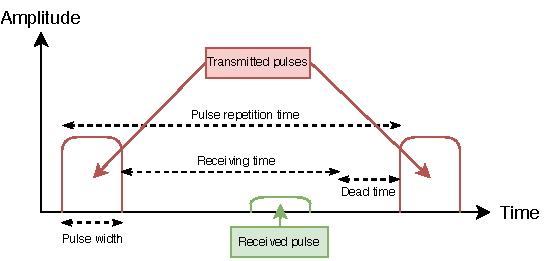
\includegraphics[width=0.8\textwidth]{figures/background/pulsed_radar.pdf}
    \caption{Pulsed radar time amplitude figure.}
    \label{fig:pulsed_radar}
\end{figure}

Radar is a sensing system that is used to detect targets using radio waves \cite{Curry2011}.
Transmitter (TX) emits radio waves towards desired directions, and a receiver (RX) is used to receive radio waves reflected from surfaces and scattered off the targets. 
The reflected or scattered waves are often called echoes.
Radar Cross-Section (RCS) determines the fraction of electromagnetic energy scattered from the target in the direction of the receiver \cite{Curry2011}.
The target RCS depends on the target shape and materials as well as on radio wave frequency, viewing angles, and signal polarization.
The target RCS has a unit of square meter sm (or m$^2$) and often described in decibels by dBsm.

The echoes produced from other sources than targets of interest are called clutter.
The received signal is corrupted by clutter, additive noise from the receiver electronics, and possibly also by unintentional or intentional interferences from other radio systems \cite{Curry2011}.
In modern radar systems, signal processing algorithms are utilized to perform target detection from the corrupted received signal \cite{Mahafza2015}.
Typical detection algorithms are based on matched filtering and hypothesis testing \cite{Mahafza2015}.

There are two types of radar systems when categorized based on the waveform used.
These systems are pulsed-wave radar systems and continuous wave radar systems \cite{Mahafza2015}.
However, only pulsed-wave radar systems are considered in the rest of the thesis.

The target range is obtained by measuring the time taken by a radio wave to propagate from a TX via target to an RX.
For a monostatic radar which has TX and RX at the same location, the range is obtained using the following equation \cite{Curry2011}
\begin{equation}
\label{eq:target_range}
    d = \frac{ v_c \tau}{2} 
\end{equation}
where $\tau$ is the propagation delay and $v_c$ is speed of light.
When object is moving towards or away from the receiver, a Doppler frequency shift is induced to the radio wave according to the following equation \cite{Curry2011}
\begin{equation}
\label{eq:doppler_freq}
    f_d = \frac{2 f v_r}{v_c},
\end{equation}
where $f$ is the transmit frequency, and $v_r$ is the radial velocity towards the receiver.
The shift can be utilized for determining moving target echoes from the stationary clutter echoes \cite{Curry2011}.
The Doppler shift can also be utilized to measure the range-rate, i.e., the radial velocity of the target \cite{Curry2011}.

Typical techniques for measuring the target elevation and azimuth coordinates are conical scan, sequential lobing, and monopulse techniques \cite{Sherman2011}. 
The former two techniques are based on moving the beamlobe around the target, and the amplitude of the received echoes are examined. 
From the power intensity of the echoes, it is possible to estimate the target angle.
However, fluctuations in target returns create false indications of the target angle \cite{Sherman2011}.
Monopulse techniques avoid this problem by inferring the target angle from a single pulse \cite{Sherman2011}.
In the amplitude-comparison monopulse technique, the beamlobe is divided into sub-beams that are slightly off-axis compared to the boresight axis.  
The received signal power is compared between the sub-beams to infer the target angle; thus, only a single pulse is required to obtain the measurement.
On the other hand, the phase-comparison monopulse technique measures the target angle by examining the phases of the signals received at antennas closely spaced from each other \cite{Sherman2011}.

Pulsed wave radar systems detect targets by transmitting a train of pulses \cite{Mahafza2015}.
Figure \ref{fig:pulsed_radar} illustrates the transmitted pulses and received echoes.
The time between subsequent pulses is called Pulse Repetition Time (PRT). 
Furthermore, Pulse Repetition Frequency (PRF) stands for the reciprocal of PRT.
As shown in Figure \ref{fig:pulsed_radar}, PRT is determined by pulse duration and receiving time.
Pulse duration affects the amount of energy that will be transmitted.
With higher energy, it is easier to detect the targets.
The pulse duration also affects the range resolution, which defines how well two closely spaced targets can be separated \cite{Curry2011}.
Receiving time determines the maximum unambiguous range detectable by the radar.
If the target is at a longer range than the maximum unambiguous range, the received pulse is not the most recent transmitted pulse such that the propagation delay $\tau$ could not be correctly calculated \cite{Curry2011}.

Signal-to-Noise Ratio (SNR) of a radar can be calculated using the following equation \cite{Curry2011}
\begin{equation} \label{eq:radar_snr}
SNR = \frac{P_p G_T \psi G_R l^2 C}{(4\pi)^3 d_\text{tx}^2 d_\text{rx}^2 W k T_s L},
\end{equation}
where
\begin{itemize}
    \item $P_p$ is the peak transmit power,
    \item $G_T$ is the transmit antenna gain,
    \item $\psi$ is the target RCS,
    \item $G_R$ is the receive antenna gain,
    \item $l$ is the wavelength,
    \item $C$ is the pulse compression gain,
    \item $d_\text{tx}$ is the target range from transmitter,
    \item $d_\text{rx}$ is the target range from receiver,
    \item $W$ is the radar signal bandwidth,
    \item $k$ is Boltzmann's coefficient,
    \item $T_s$ is the system noise temperature, and 
    \item $L$ is the additional radar system loss factor.
\end{itemize}
The pulse compression gain $C$ depends on the waveform used.
The system loss factor $L$ includes any additional losses originated from the environment or the radar system.

Other factors that affect the SNR are interference and pulse integration \cite{Curry2011}.
Signals received by the radar but originating from outside the radar system are considered interference.
Thus, the signal-to-interference-plus-noise ratio (SINR) has a form of $\frac{S}{N+I}$, where
$S$ is the signal power,
$N$ is the thermal noise power, and
$I$ is the received power of the interference.
However, the interference may also be intentional and have properties different from random noise. 
Pulse integration denotes to combining multiple signal returns to get higher SNR.
The SNR gain factor depends on whether coherent or non-coherent integration is used.
Coherent integration means that phase information can be preserved. 
Thus the returns can be integrated with aligned phases \cite{Curry2011}.

The radars steer the transmitted radio waves into the desired direction, either mechanically by rotating the transmit antenna \cite{Curry2011} or using electronically steerable antennas, which are based on a phased array technology \cite{Mailloux2017}.
Mechanically steerable radar systems typically rotate with constant angular velocity, such that each azimuth-elevation bin is revisited with a constant revisit time.
An electronically steerable phased array can be steered in any direction with a relatively low delay within the field of view.
Thus, RRM for ESA radars has more degrees of freedom for controlling the beam pattern.


\subsection{Radar configurations} \label{sec:radar_types}

\begin{figure}[htb]
    \centering
    \begin{subfigure}[b]{0.45\textwidth}
        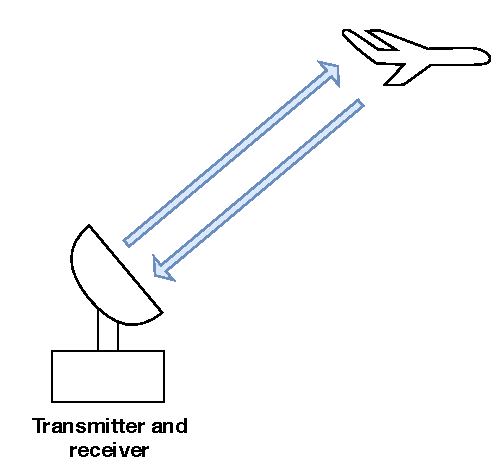
\includegraphics[width=0.7\textwidth]{figures/background/radar_types_monostatic.pdf}
        \caption{Monostatic radar.}
        \label{fig:monostatic_radar}
    \end{subfigure}
    \hfill
    \begin{subfigure}[b]{0.45\textwidth}
        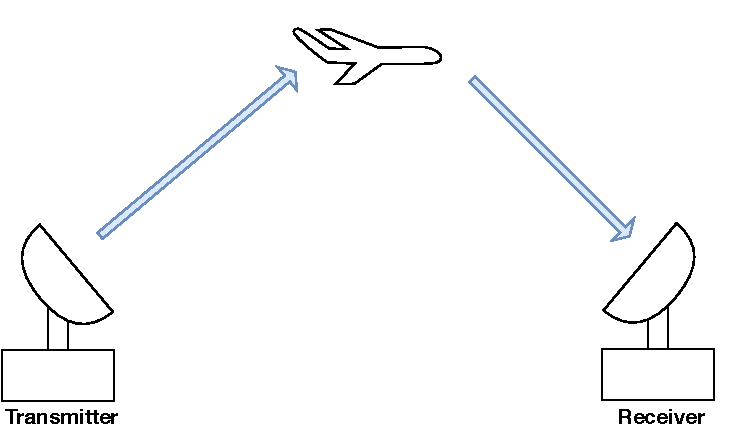
\includegraphics[width=\textwidth]{figures/background/radar_types_bistatic.pdf}
        \caption{Bistatic radar.}
        \label{fig:bistatic_radar}
    \end{subfigure}
    \hfill
    \begin{subfigure}[b]{0.45\textwidth}
        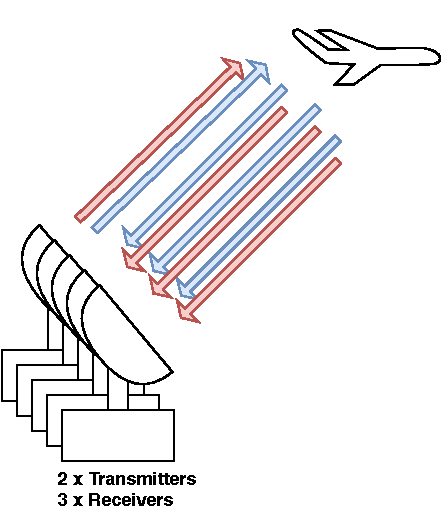
\includegraphics[width=0.7\textwidth]{figures/background/radar_types_colocated_MIMO.pdf}
        \caption{Example of MIMO radar with colocated antennas.}
        \label{fig:colocated_MIMO_radar}
    \end{subfigure}
    \hfill
    \begin{subfigure}[b]{0.45\textwidth}
        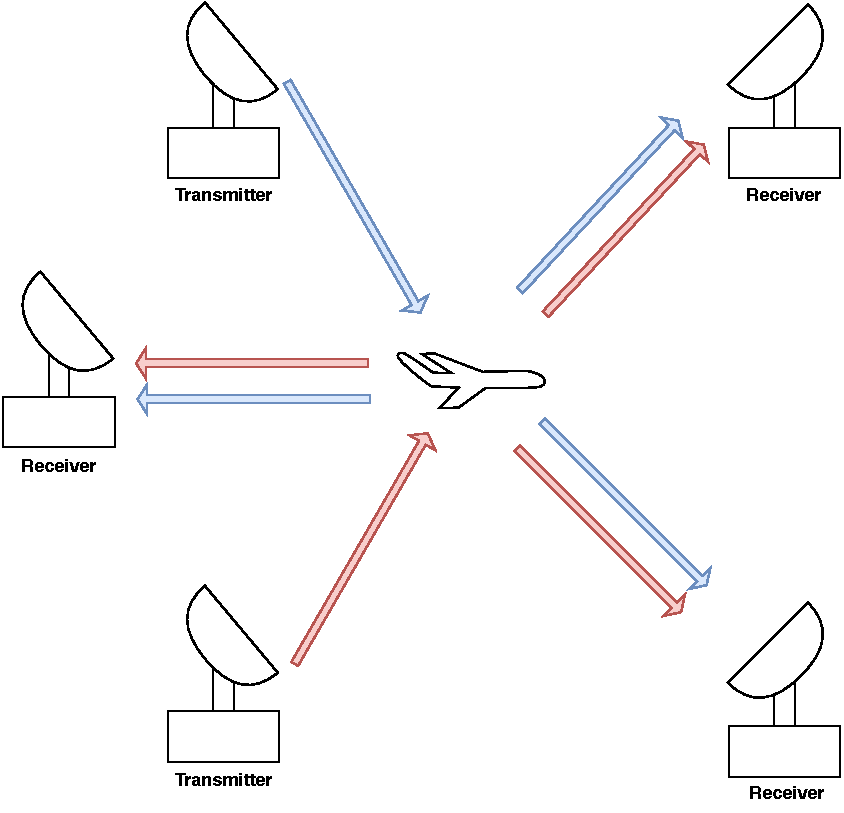
\includegraphics[width=\textwidth]{figures/background/radar_types_distributed_MIMO.pdf}
        \caption{Example of MIMO radar system with distributed antennas.}
        \label{fig:distributed_MIMO_radar}
    \end{subfigure}
    \caption{Different radar configurations. An arrow illustrate propagation of a waveform from a transmitter to a receiver.}
    \label{fig:radar_types}
\end{figure}

In general, radar systems can be divided into three configuration classes: monostatic radars, bistatic radars, and multistatic radars.
Monostatic radar systems have a single radio unit that can transmit and receive radio waves, as shown in Figure \ref{fig:monostatic_radar}.
The bistatic radar system has a TX unit and an RX unit which are distant from each other, as shown in Figure \ref{fig:bistatic_radar}.
Furthermore, a multistatic radar system is a radar network that has multiple transmitters and receivers.
The individual radar components can be either monostatic radars or bistatic radars.
In multistatic radar systems, each radar component functions independently, and only high-level products of local processing are given for the central processor.

Similar to multistatic radars are Multiple-Input Multiple-Output (MIMO) radars, but the designation is used to distinguish the difference in designing and processing the multiple waveforms jointly \cite{Haimovich2008}.
Therefore, in the MIMO radars, each transmitter-receiver (TX-RX) pair forms an independent channel for illuminating and observing the targets.
MIMO radars can be further divided into the following subclasses: MIMO radars with colocated antennas \cite{Li2007}, and MIMO radars with widely separated antennas \cite{Haimovich2008}.
The subclasses will be called colocated MIMO radars and distributed MIMO radars, respectively.

Colocated MIMO radars have multiple antennas closely located to each other.
Compared to phased-array monostatic radars, the MIMO radar technology improves the parameter estimation capabilities, and enhance the flexibility in beampattern design \cite{Li2007}.
It may transmit multiple different waveforms simultaneously, whereas phased-array radar sends the same waveform from each antenna with an appropriate delay.
An example of a colocated MIMO radar with two TXs antennas and three RXs antennas is shown in Figure \ref{fig:colocated_MIMO_radar}.
In distributed MIMO radar systems, multiple TXs and RXs are deployed in different locations.
The distances between the antennas are longer than coherence distance such that the radar channels are not correlated \cite{Haimovich2008}.
The widely distributed antennas increase spatial diversity, which can be utilized to improve target localization accuracy and detect low-observable targets.
An example of a distributed MIMO radar with two TXs and three RXs is shown in Figure \ref{fig:distributed_MIMO_radar}.

\subsection{Target tracking with radars} \label{sec:Tracking}

Radars acquire observations that are processed to obtain, for example, the target position and the range-rate, as discussed in Section \ref{sec:radar_opertaion_principle}.
A state of a target can be modeled as a continuous-valued stochastic process that evolves based on the target kinematics. 
Typically, the measurements of the state variables are noisy and all the state variables can not be directly measured.
Therefore, target tracking algorithms are utilized to filter the observation history to attenuate noise, as well as to estimate the present state and predict future states.
Typical target tracking algorithms are based on a statistical model that combines a motion model and a measurement model. 
Such models are known as state-space models \cite{RongLi2003}.

The motion model describes how the kinematic state of a target $\x$ evolves through time.
In general, the notation $\x$ is short hand for $\vec{x}_{t_k}$ which means value of $\vec{x}$ at time instant $t_k$. 
A discrete-time motion model may be expressed as follows \cite{RongLi2003}
\begin{equation}\label{eq:spm_motion}
    \xnext  = f(\x, \cinput) + \pnoise,
\end{equation}
where $f(\x, \cinput)$ is a deterministic function of the state $\x$ and control input $\cinput$.
The variable $\pnoise$ models noise that describes uncertainty in the model, and it is called the process noise.
The measurement model is used to describe the relationship between the target state and the observation $\z$. 
Similar to the motion model, the discrete-time measurement model is written as follows \cite{RongLi2003}
\begin{equation}\label{eq:spm_obs}
    \z = h(\x) + \onoise,
\end{equation}
where $h(\x)$ maps the state to the observation, and $\onoise$ is the measurement noise.

\subsubsection{Target motion models} \label{sec:target_models}

Different kinds of target motion models have been developed to mimic real target motion with a desired accuracy. 
Commonly used motion models include Constant Velocity (CV), Constant Acceleration (CA), and Coordinated Turn (CT) models \cite{RongLi2003}.
On a higher level, the models can be divided into non-maneuvering and maneuvering models \cite{RongLi2003}. 
Non-maneuvering motion means that the target velocity and elevation remain approximately constant, and otherwise, the motion is considered as a maneuver.
The state transition function $f(\x, \cinput)$ is based on the physics of the target dynamics, where the control input $\cinput$ is typically unknown.
In addition, the statistical parameters of the process noise $\pnoise$ are typically unknown.
Thus, the unknowns need to be estimated or chosen reasonably.

Specific CV and CA target motion models are introduced here.
The models are based on the assumption that target acceleration is white Gaussian noise and decoupled between each spatial dimension.
The two target motion models are called
\begin{enumerate}
    \item Discrete White Noise Acceleration (DWNA) model, and
    \item Discrete Wiener Process Acceleration (DWPA) model \cite{BarShalom2001}.
\end{enumerate}
The aforementioned target models can be expressed with linear combinations as follows
\begin{equation}
    \vec{x}_{k+1} = \mathbf{F}_k \vec{x}_k + \vec{g} w_k,
\end{equation}
where $\vec{g}$ is a vector and $w_k \in \normal{0}{\sigma_w^2}$ Gaussian random variable with zero mean and variance of $\sigma_w^2$.
The state transition matrix $\mathbf{F}_k$ can be derived by solving differential equations up to the first order for the DWNA model and the second order for the DWPA model.
The DWNA model is used to model target motion when the target moves with nearly constant velocity; thus, this model is referred to as the CV model.
On the other hand, DWPA models the target motion when the acceleration may last for a more extended period. 
Therefore, the model is referred to as the CA model.

The following equations are written for target motion in two dimensional (2D) space, and
the notation for time instance $k$ is omitted, and superscripts $1$ and $2$ denote CV and CA models, respectively. 
In addition, notation $\dot{x}$ is used to denote the first order derivative $\frac{\partial x}{\partial t}$, and similarly $\ddot{x}=\frac{\partial^2 x}{\partial t^2}$ is the second order derivative.
The state of the CV model in a 2D space is expressed as follows
\begin{equation}\label{eq:x_mode1}
    \hat{\mathbf{x}}_1 =
        \transpose{
        \begin{pmatrix}
            x & \dot{x} & y & \dot{y}
    \end{pmatrix}},
\end{equation}
where $x$ and $y$ are target coordinates along x and y axes. 
Since the state transitions along each coordinate are decoupled, a model for one dimensional (1D) space is utilized to simplify the notation.
In 1D space, the state transition matrix is defined as follows
\begin{equation}\label{eq:f_mode1}
    \Tilde{\vec{F}}_1 =
    \begin{pmatrix}
        1 & \dt \\
        0 & 1  \\
    \end{pmatrix},
\end{equation}
where $\dt=t_{k+1} - t_k$ is the time step.
The Gaussian random variable $w$ affects the state transition via the following vector
\begin{equation}\label{eq:g_noise_mode1}
\vec{g}_1 =\transpose{\begin{pmatrix}
        \frac{1}{2} \dt^2 & \dt
    \end{pmatrix}}
\end{equation}
which is derived by integrating position and velocity for the constant acceleration $w$ lasting for time period of $\dt$.
The process noise covariance matrix is calculated as follows  
\begin{equation}
    \Tilde{\vec{Q}}_1 = \sigma_w^2 \vec{g}_1 \transpose{\vec{g}_1}
    = \sigma_w^2
    \begin{pmatrix}
        \frac{1}{4} \dt^4 & \frac{1}{2} \dt^3 \\ 
        \frac{1}{2} \dt^3 & \dt^2 \\ 
    \end{pmatrix},
\end{equation}
where $\sigma_w^2$ is the variance of the Gaussian random variable $w$.
In 2D space, the state transition matrix and process noise covariance matrix can be expressed as block diagonal matrices as follows 
\begin{equation}\label{eq:F_mode1}
\vec{F}_1 = \diag{\Tilde{\vec{F}}_1, \Tilde{\vec{F}}_1}
\end{equation}
and
\begin{equation}
    \vec{Q}_1 = \diag{\Tilde{\vec{Q}}_1, \Tilde{\vec{Q}}_1}.
\end{equation}
where the operator $\diag{\cdot}$ creates a block diagonal matrix from the given matrices.

The CA model is similar to the CV model, but the order of the kinematic state is increased.
In other words, accelerations along each coordinate are included into the state as follows  
\begin{equation}\label{eq:x_mode2}
    \hat{\mathbf{x}}_2 =
        \transpose{
        \begin{pmatrix}
            x & \dot{x} & \ddot{x} & y & \dot{y} & \ddot{y}
        \end{pmatrix}}.
\end{equation}
The state transition matrix and process noise covariance matrix for the CA model are written as follows
\begin{equation}\label{eq:f_mode2}
    \Tilde{\vec{F}}_2 = 
    \begin{pmatrix}
        1 & \dt & \frac{1}{2}\dt^2  \\ 
        0 & 1 & \dt \\
        0 & 0 & 1  \\
    \end{pmatrix}
\end{equation}

\begin{equation}
    \vec{g}_2 = \transpose{
        \begin{pmatrix}
            \frac{1}{2} \dt^2 & \dt & 1
        \end{pmatrix}
    }
\end{equation}

\begin{equation}
    \Tilde{\vec{Q}}_2 = \sigma_w^2 \vec{g_2} \transpose{\vec{g_2}}  =  \sigma_w^2
        \begin{pmatrix}
            \frac{1}{4} \dt^4 & \frac{1}{2} \dt^3 & \frac{1}{2} \dt^2 \\ 
            \frac{1}{2} \dt^3 & \dt^2 &  \dt \\
            \frac{1}{2} \dt^2 & \dt & 1
        \end{pmatrix}
\end{equation}

\begin{equation}\label{eq:F_mode2}
\vec{F}_2 = \diag{\Tilde{\vec{F}}_2, \Tilde{\vec{F}}_2}
\end{equation}
\begin{equation}
    \vec{Q}_2 = \diag{\Tilde{\vec{Q}}_2, \Tilde{\vec{Q}}_2}
\end{equation}
which are based on the same principles that was shown for the CV model.

\subsubsection{Radar measurement model} \label{sec:measurement_model}

In this section, a measurement model is introduced for monostatic radars.
This model is suitable for linear trackers when using the target models presented is Section \ref{sec:target_models}.
The linearity also implies that the range-rate measurements are not used.

It is assumed that the monostatic radar obtains the position measurements in polar coordinates, and the measurements are distorted by uncorrelated Gaussian noise.
Thus, noisy estimates of range $d$, azimuth angle $\theta$, and elevation angle $\beta$ are obtained, where the unit of angular measurements is the radian. 
The polar coordinates are converted into Cartesian coordinate system using the following conversion equations:
\begin{equation}
\left\{
\begin{array}{l}
    x = d \cos(\theta) \cos(\beta) \\
    y = d \sin(\theta) \cos(\beta) \\
    z = d \sin(\beta).
\end{array}\right.
\end{equation}
After converting the radar measurements into the Cartesian coordinate system, the measurement model $h(\x)$ in equation \eqref{eq:spm_obs} can be expressed with linear combinations $h(\x) = \omodel \x$.
For CV state in equation \eqref{eq:x_mode1} and CA state in equation \eqref{eq:x_mode2}, the measurement matrix $\omodel$ is defined as follows
\begin{equation}\label{eq:position_measurement_matrix}
    \omodel = 
       \begin{pmatrix}
            1 & \vec{0}_{1, n} & \vec{0}_{1, n+1}\\ 
            \vec{0}_{1, n+1} & 1 & \vec{0}_{1, n}\\ 
        \end{pmatrix}
\end{equation}
where $n$ is the order of the motion model, and $\vec{0}_{i,j}$ is zero matrix with size of $i\times j$.

The measurement model needs to be linearized to obtain the measurement noise covariance matrix in the Cartesian coordinate system.
The approximation shown here is for 2D space.
Assume that target is at position $x=d$ and $y=0$, then $\Var{x}$ = $\Var{d} = \sigma_d^2$, and variance along y-axis can be linearized as follows
\begin{equation*}
    \Var{y} \approx \Var{d \sin\left(\theta\right)} \approx \Var{d \theta} = d^2\sigma_\theta^2,
\end{equation*} 
for small values of $\sigma_\theta^2$, which is the error variance along the azimuth angle.
For arbitrary azimuth angle, the variance components need to be rotated as follows
\begin{equation} \label{eq:cartesian_measurement_covariance}
    \ocov = \rotmat 
    \begin{pmatrix}
            \sigma_d^2 & 0 \\
            0 & d^2 \sigma_\theta^2
    \end{pmatrix}
    \transpose{\rotmat},
\end{equation}
where $\rotmat$ is the 2D rotation matrix
\begin{equation}
    \rotmat = 
    \begin{pmatrix}
            \cos(\theta) & -\sin(\theta) \\
            \sin(\theta) & \cos(\theta)
    \end{pmatrix}.
\end{equation}
For a monopulse radar \cite{Sherman2011}, the measurement noise variances for range $\sigma_d^2$ and angle $\sigma_\theta^2$ can be calculated using the equations \cite{Curry2011}
\begin{equation}
    \sigma_d^2 =  \frac{d_\text{res}^2}{2 SNR}  \label{eq:sigma_r}\\
\end{equation}
and
\begin{equation}
    \sigma_\theta^2 =  \frac{2 B^2}{k_m^2 SNR} \label{eq:sigma_theta},
\end{equation}
where $d_\text{res}$ is range resolution, and $B$ is half of the -3dB beamwidth. 
The parameter $k_m$ is a monopulse antenna pattern difference slope, which is a specific property of a monopulse beamlobe that affects the accuracy of the angle measurements \cite{Sherman2011}.
The equations \eqref{eq:sigma_r} and \eqref{eq:sigma_theta} require the SNR to be estimated.

\subsubsection{Kalman filters for target tracking} \label{sec:kalman_filter}

\begin{figure}[b]
    \centering
    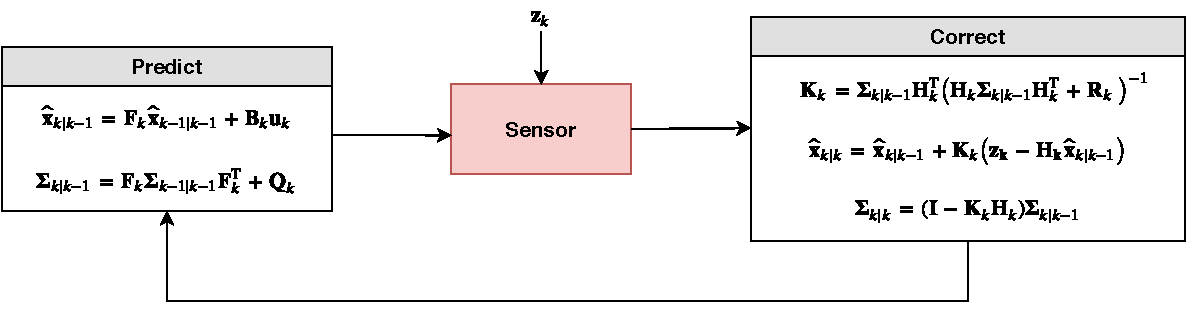
\includegraphics[width=\textwidth]{figures/KF.pdf}
    \caption{The Kalman filtering phases.
    First, the predictive estimates are calculated.
    Then, the predictive estimates are corrected using the new information in the measurement $\z$ to get the filtered estimates.
    }
    \label{fig:KF}
\end{figure}

Kalman filtering is a Minimum Mean Square Error (MMSE) state estimation algorithm for linear state-space systems \cite{Zarchan2000}.
The discrete-time linear state-space model is expressed using linear combinations as follows \cite{Zarchan2000}
\begin{align}
    \xnext &= \stmodel \x + \cimodel \cinput + \pnoise \label{eq:lsp_state} \\
    \z &= \omodel \x + \onoise \label{eq:lsp_obs}
\end{align}
where $\stmodel$ is state transition matrix, $\cimodel$ is control-input matrix, $ \omodel $ is observation matrix. 
The noise statistics are described with zero mean Gaussian distributions $\pnoise \sim \normal{0}{\pcov}$ and $\onoise \sim \normal{0}{\ocov}$, where $\pcov$ is the process noise covariance matrix and $\ocov$ is the measurement noise covariance matrix.
Kalman filtering is optimal when the state-space model matches the real system, the noises are Gaussian and uncorrelated, and the noise covariances are known \cite{Zarchan2000}.

The Kalman filtering can be divided into two distinct phases, as shown in Figure \ref{fig:KF}.
In the first phase, the next state is predicted from the previous estimate using the expectation of the equation \eqref{eq:lsp_state}.
The predicted estimates are also called \prior estimates.
Filtered or \post estimate of the state is obtained at time instance $k$ after observing $\z$ and using the new information in the measurement for correcting the predicted estimate. 
The notation $k|k-1$ is used to denote the \prior estimates and $k|k$ denote \post estimates.
The \prior error covariance matrix $\priorecov$, which estimates the accuracy of the state estimates $\xprior$, is updated based on the process noise covariance matrix and the previous estimated \post error covariance matrix.
The prediction phase can be expressed with two equations as follows \cite{Zarchan2000},
\begin{align}
    \xprior &= \stmodel \xlast + \cimodel \cinput \label{eq:kf_pred_x} \\ 
    \priorecov &= \stmodel \lastecov \stmodel^T + \pcov \label{eq:kf_prior_error_cov},
\end{align}
where $\xlast$ is the previous \post state estimate, and $\lastecov$ the corresponding \post error covariance matrix.

In the second phase, a measurement is obtained, and the \prior estimate is corrected using the measurement $\z$ and the Kalman gain $\gain$.
The update phase starts by calculating a residual between the observation $\z$ and the predicted observation $\zhat = \omodel \xprior$, which is the expectation of the observation equation \eqref{eq:lsp_obs}.
The residual $\z-\zhat$ is called innovation, and it is utilized to correct the \prior estimate $\xprior$.
The Kalman gain defines how much the innovation is weighted to correct the predicted estimate $\xprior$.
If the measurement error covariance is high, the measurements can be trusted less compared to the situation where the measurement error covariance is low.
Thus in the former case, the Kalman gain corrects the estimates less than in the latter case.
The Kalman gain is found by minimizing the Mean Square Error (MSE) between $\x$ and $\xpost$.
As a result, following update equations are obtained \cite{Zarchan2000}

\begin{align}
    \prefitinnov &= \z - \omodel \xprior \label{eq:kf_prefit_innov}\\ 
    \innocov &= \omodel \priorecov \omodel^T + \ocov \label{eq:kf_innov_cov}\\ 
    \gain &= \priorecov \omodel^T \inv{\innocov} \label{eq:kf_gain}\\ 
    \xpost &= \xprior + \gain \prefitinnov \label{eq:kf_update_x}\\ 
    \postecov &= \left( \eye - \gain \omodel \right) \priorecov  \label{eq:kf_post_error_cov}
\end{align}
where $\innocov$ is the covariance matrix of the innovation $\prefitinnov$. 
Even if the notation in the prediction and update equations does not explicitly suggest it, multiple predictions can be made recursively using \prior estimates, or multiple updates can be made at each time instance.

\subsubsection{Interacting multiple model estimator}
\label{sec:IMM}

\begin{figure}[t]
    \centering
    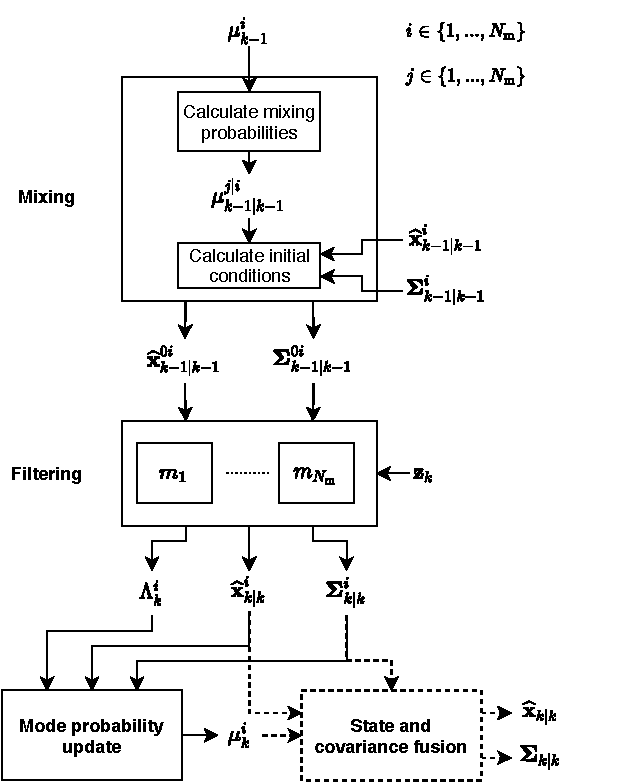
\includegraphics[width=0.7\textwidth]{figures/IMM.pdf}
    \caption{
    The four stages of a IMM estimator \cite{BarShalom2001}.}
    \label{fig:IMM}
\end{figure}

In a realistic scenario, the target motion can follow different modes, and the changes between the modes are controlled by an external agent, for example, by a human.
Such systems are called hybrid systems. 
Those are characterized by a continuous-time stochastic process, such as equation \eqref{eq:spm_motion}, that describes the motion model for each mode, and by a discrete-time stochastic process that describes the evolution of the modes \cite{BarShalom2001}.
Thus, the target mode designates the specific behavior of a target, which is modeled with a target motion model.

The multiple model approach, in which numerous target models are concurrently used for tracking, has emerged to track the hybrid systems effectively \cite{BarShalom2001}.
The approach assumes that target motion obeys one of the modes from a finite set of modes at a time.
However, in real-word trackers, the target motion models are chosen to approximate the underlying modes \cite{Simeonova2002}.
The underlying mode is identified by a mode-matched filter, which calculates the probability for each mode given the past observations.
For an optimal approach, the number of mode matched filters would grow exponentially as a function of time, even if the modes are switched based on a hidden Markov model (HMM) \cite{BarShalom2001}.
The HMM is presented in more detail in Chapter \ref{sec:RL}.
An Interacting Multiple Model (IMM) estimator is a specific suboptimal hybrid filter that achieves a significant trade-off between the performance and the computational complexity \cite{BarShalom2001}.

An IMM estimator assumes that the target motion at each time instance is following one of the modes in the countable set $\mathcal{M} = \{ m_i \}_{i=1}^\nmodels$, where $\nmodels$ is the number of the alternate modes \cite{BarShalom2001}.
In addition, it is assumed that each mode can be modeled with a target motion model.
The modes transition according to an HMM, and the state transition probabilities of the HMM are assumed to be known.
However, in practical scenarios, the target motion models and the transition probabilities are considered as design parameters \cite{Simeonova2002}.
Given $\mathcal{Z}_k$, which is the observation sequence until time instance $k$, the posterior probability for mode $m_i$ to be in effect at time instance $k$ is written as $\modeprob = \Pr{M_k=m_i | \mathcal{Z}_k}$, where $M_k$ is the mode in effect at time instance $k$.
The probability is later referred to as mode probability.

The IMM estimator can be summarized with four stages that are shown in Figure \ref{fig:IMM}.
The stages are mixing, filtering, mode probability update, and state and covariance combination. 
The stages are further implemented as follows.


\begin{description}
% ---------------------------------------------------------
% Mixing
% ---------------------------------------------------------
\item[Mixing.]

Mixing probability is defined as follows
\begin{equation}\label{eq:mixing_conditional_prob}
    \lastmxprobs = \Pr{M_{k-1}=m_j|M_{k}=m_i, \mathcal{Z}_{k-1}},
\end{equation}
which is the probability for a target following mode $m_j$ at time instance $k-1$ if target is following the mode is $m_i$ at time instance $k$ given the observations up to time instance $k-1$.
The equation \eqref{eq:mixing_conditional_prob} can be written into form
\begin{equation}
    \lastmxprobs = \frac{1}{\mxnorm} P_{ji} \mu^j_{k-1} \label{eq:imm_mx_probs}
\end{equation}
where $P_{ji}$ is the probability of the mode $m_j$ switching to the mode $m_i$, and $\mxnorm$ is defined as follows
\begin{equation}
    \mxnorm = \sum_j^\nmodels P_{ji} \mu^j_{k-1}. \label{eq:imm_mx_normalization}
\end{equation}
The mixing probabilities are used to calculate mixed estimates for the most recent posterior state variables and error covariance matrices, which are further used in the tracking filters.
Moreover, the mixed estimates are calculated for each tracking filter by assuming that the current mode of the target matches to the motion model of the tracking filter, as described by equation \eqref{eq:mixing_conditional_prob}.
Therefore, the mixed state and estimation error covariance matrices at time instance $k-1$ are calculated as follows
\begin{align}
    \xmxinit &= \sum_j^\nmodels \lastmxprobs \modexlast \label{eq:imm_mx_init_x}\\
    \ecovmxinit &= \sum_j^\nmodels \lastmxprobs \left[ \modecovlast + \modemxcovlast \right], \label{eq:imm_mx_init_P}
\end{align}
where $\modexlast$ and $\modecovlast$ are the previous filtered state and covariance estimates of the tracking filter of mode $m_j$, respectively. 
In addition, $\modemxcovlast$ is defined as follows
\begin{equation}
    \modemxcovlast = 
    \left( \xmxinit - \modexlast  \right) 
    \transpose{\left( \xmxinit - \modexlast   \right)}.\label{eq:imm_mx_init_Ptilde}
\end{equation}

% ---------------------------------------------------------
% Filtering
% ---------------------------------------------------------
\item[Filtering.]

In the filtering phase, the probability density $\modeobsprob = p\left( \z | M_k = m_i, \mathcal{Z}_{k-1} \right) $ is calculated, which is the probability density of the observation $\z$ when mode $m_i$ is assumed active at time instance $k$ and observation history up to time instance $k-1$ is given.
The conditioning is approximated by assuming that $\xmxinit$ and $\ecovmxinit$ can be used to condition the filters before propagating the filtering equations.
Therefore, probability densities for each mode $\modeobsprob$ are obtained using a Gaussian distribution $\normal{\modexprior}{\modeinnovcov}$.
The predicted state $\modexprior$ is calculated using equations \eqref{eq:imm_mx_init_x} and \eqref{eq:kf_pred_x}.
Furthermore,  $\modeinnovcov$ is calculated using equations \eqref{eq:imm_mx_init_P}, \eqref{eq:kf_prior_error_cov} and \eqref{eq:kf_innov_cov}.

% ---------------------------------------------------------
% Mode probability update
% ---------------------------------------------------------
\item[Mode probability update.]

The mode probabilities $\mu^i_k$ are updated by using the probability densities $\Lambda_k^i$ as follows
\begin{equation}
    \mu_k^i = \frac{1}{c} \Lambda^i_k \mxnorm,
\end{equation}
where
\begin{equation}
    c = \sum_{i=1}^\nmodels \Lambda_k^i \mxnorm
\end{equation}
is a normalization constant.

% ---------------------------------------------------------
% State and covariance fusion
% ---------------------------------------------------------
\item[State and covariance fusion.]
Lastly, the posterior estimates $\xpost$ and $\postecov$ can be updated by weighting the \post estimates of each filter with the mode probabilities.
Thus, the estimates are calculated as follows
\begin{align}\label{eq:imm_fusion_x}
    \xpost =& \sum_{i=1}^\nmodels \mu_k^i \modexpost\\
\label{eq:imm_fusion_P}
    \postecov &= \sum_{i=1}^\nmodels \mu_k^i 
    \left[ 
        \modecovpost + \left( \modexpost - \xpost \right) \transpose{\left( \modexpost - \xpost \right)}
    \right].
\end{align}
Note that the equations \eqref{eq:imm_fusion_x} and \eqref{eq:imm_fusion_P} are outputs of the IMM estimator, and not needed for the other IMM estimator stages.
\end{description}


\newpage
\section{Reinforcement Learning} \label{sec:RL}

\begin{figure}[b]
    \centering
    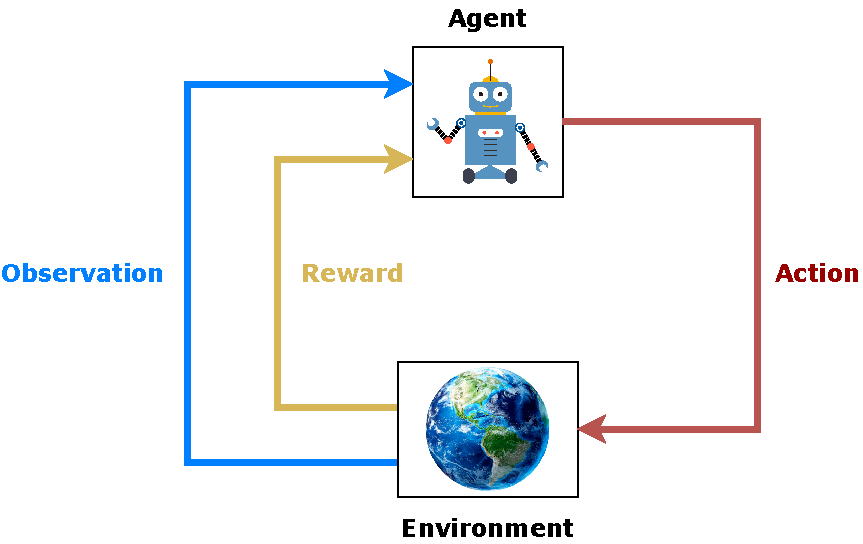
\includegraphics{figures/RL_diagram.pdf}
    \caption{Reinforcement learning.}
    \label{fig:RL_basics}
\end{figure}

Reinforcement Learning (RL) is a method for learning to act in stochastic sequential decision-making problems without a model developed beforehand that describes the problem dynamics \cite{Sutton2018}.
In RL, an agent interacts with an environment by taking different actions.
After taking an action, the agent observes the environment state and receives a scalar reward that quantifies the quality of the action.
Given the state of the environment, the agent takes the next action. 
The differences between the observations and the states are described in sections \ref{sec:MDP} and \ref{sec:POMDP}.
The learning is based on a trial and error approach, which is controlled through the rewards.
The agent independently improves its performance by reasonably probing different actions for different states to learn their consequences to future rewards.
Thus, RL problems are based on rewards, observations, and actions, as shown in Figure \ref{fig:RL_basics}.

Rewards are defined such that the objective is achieved by maximizing the sum of future rewards \cite{Sutton2018}.
For example, if an RL method is used to teach a robot to play chess, a positive reward should be given if the robot wins, and otherwise, no reward is obtained.
Then, the sum of future rewards indicates the probability of winning given the current state of the game.
In some cases, it is more reasonable to use negative rewards.
For instance, if the objective is to minimize the number of steps needed to get out of a maze. 
Then negative reward could be given for each step that emphasizes the agent to learn a policy for taking a minimum amount of steps to get out of the maze.

RL algorithms are based on a Markov Decision Process (MDP) framework in which state transition probabilities and reward distributions are unknown.
Therefore, this chapter is organized as follows.
Section \ref{sec:MC} introduces a Markov chain, which is a fundamental component in an MDP.
Furthermore, MDPs are described in Section \ref{sec:MDP}.
Typical Radar Resource Management (RRM) problems are Partially Observable Markov Decision Processes (POMDP) in which the MDP state is not fully observable. 
Thus a brief introduction to POMDPs is given in Section \ref{sec:POMDP}.
Exploration-exploitation dilemma is one of the fundamental concepts in RL. Therefore, the exploration-exploitation trade-off is introduced in Section \ref{sec:exp_exp}. 
Lastly, a particular RL algorithm, named Q-learning, is presented in Section \ref{sec:q_learning}.


\subsection{Markov chains} \label{sec:MC}

\begin{figure}[b]
    \centering
    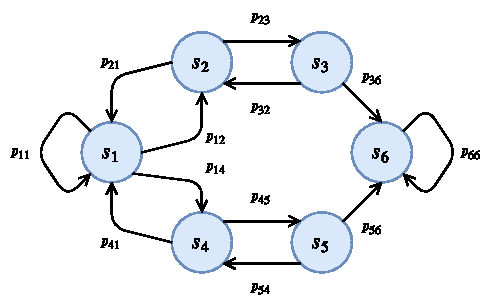
\includegraphics[width=0.8\textwidth]{figures/MarkovChain.pdf}
    \caption{
    An example of a Markov chain with six states. 
    A non-zero state transition probability from state $s_i$ to $s_j$ is written as $P_{ij}$.
    The state transition probability is zero if no arrow exists between a state pair. }
    \label{fig:mc}
\end{figure}


Consider an environment that has a finite number of states.
The set of all different states is denoted by $\Ss$, which is also called state space.
The state of the environment can sequentially transition from one state to another based on a particular stochastic model.
A Markov chain is a stochastic model that can model the sequential state transitions if the transitions are memoryless.
A memoryless transition means that the following equation will hold   
\begin{equation} \label{eq:markov_property}
    \Pr{S_{k+1} | S_k, S_{k-1}, ..., S_1, S_0} = \Pr{S_{k+1} | S_k},
\end{equation}
where $S_k$ is the state at time instance $k$.
In other words, the equation \eqref{eq:markov_property} indicates that the state transition probability to state $S_{k+1}$ is only dependent on the current state $S_k$.
Thus, there is no need to remember the history of the past state transitions to determine the state transition probability.
The property in equation \eqref{eq:markov_property} is known as Markov property.

Next, the notation for the Markov chains is clarified.
A Markov chain has $\nstates$ states which are represented as $s_i \in \{s_1, s_2, ..., s_{\nstates} \}$.
If the state is a random variable, it is denoted by $S_k$ where $k$ is the time index.
For example, $S_k = s_i$ means that the state at time instance $k$ is realized as $s_i \in \Ss$. 
The state transition probability from state $s_i$ to state $s_j$ is defined as $\Pr{S_{k+1}=s_j | S_{k}=s_i}=P_{ij}$.
Moreover, it is possible to summarize the Markov chain dynamics with a state transition matrix $\stprobs$ in which the element on row $i$ and column $j$ corresponds to the probability $P_{ij}$.
An example of a Markov chain with six states is shown in Figure \ref{fig:mc}.

\subsection{Markov decision process} \label{sec:MDP}

\begin{figure}
    \centering
    \begin{subfigure}[b]{0.45\textwidth}
        \centering
        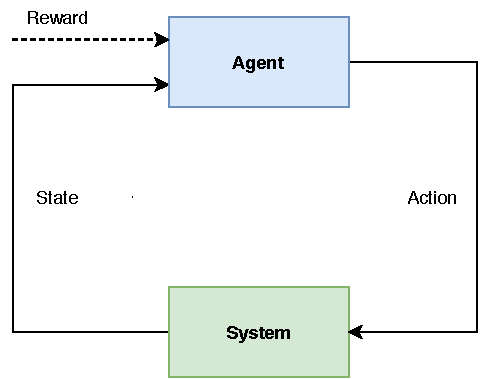
\includegraphics[width=0.9\textwidth]{figures/MDP.pdf}
        \caption{
        In an MDP, the agent takes an action that interacts with the environment.
        After the action is taken, the agent receives a reward and a new state of the environment.
        The reward can depend on the action and the state transition.
        The new environment state is used to decide the next action.}
        \label{fig:mdp}
    \end{subfigure}
    \hfill
    \begin{subfigure}[b]{0.45\textwidth}
        \centering
        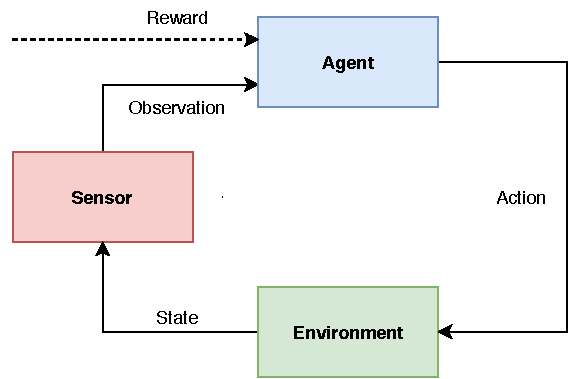
\includegraphics[width=\textwidth]{figures/POMDP.pdf}
        \caption{
        A POMDP is an extended MDP where the environment state is observed through a sensor.
        The sensor can be for example radar, and the measurements provide a noisy and partial state of the environment. 
        In comparison to the MDP, the reward function can be additionally dependent on the observations.
        }
        \label{fig:pomdp}
    \end{subfigure}
    \caption{Markov decision process (MDP) and partially observable Markov decision process (POMDP). }
    \label{fig:MDP_and_POMDP}
\end{figure}

A sequential decision process is a process where a decision-maker needs to sequentially make decisions that affect future decisions \cite{LaValle2006}.
If the outcomes of the decisions are non-deterministic, then the decision process is a stochastic sequential decision process.
A Markov decision process (MDP) is a mathematical framework used to formalize stochastic sequential decision-making problems \cite{Sutton2018}.
The decision-maker in an MDP is called an agent.

The key element of an MDP is that the environment in which the agent acts on is modeled as a Markov chain.
The agent observes the current state $s \in \Ss$ and chooses an action $a$ from a set of possible actions $\As$, which is also known as the action space.
In some cases, the possible actions are dependent on the current state.
Therefore, state-specific action space is denoted as $\As_s \subseteq \As$, which emphasizes the coupling between state $s$ and the available actions. 
The action activates a state transition of the Markov chain, and the state transition probabilities $\stprobs$ can be dependent on the action.
The action-dependent state transition probability is denoted by 
\begin{equation}\label{eq:mdp_st_prob}
    \mathrm{T}(s, s', a) = \Pr{S_{k+1}=s' | S_{k}=s , A_k=a}
\end{equation}
where $s' \in \Ss$, $a \in \As_s$, and $A_k$ is the action taken at time instance $k$.  
After the state transition, the agent receives a scalar reward.
The reward can be stochastic, and the reward distribution can be dependent on which action was taken and on the state transition.
The set of all possible rewards is a subset of real numbers $\Rs \subseteq \real$, and the subset $\Rs_{ss'}^a \subseteq \Rs$ is the set of state transition and action dependent rewards.
The dynamics of an MDP can be summarized with a single probability distribution
\begin{equation}\label{eq:MDP_probs}
    p(s', r | s, a) = \Pr{ S_{k+1}=s', R_{k+1}=r | S_k=s, A_k=a }.
\end{equation}
which is the probability that environment changes from state $s$ to state $s'$ after the action $a$ was taken and agent receives immediate reward $r \in \Rs_{ss'}^a$.

An MDP can last for a finite or infinite number of steps, and the number of steps is referred to as horizon.
From the perspective of RL theory, infinite horizon MDPs are more important \cite{Sutton2018}.
Therefore, the rest of the chapter will concentrate on them.
In an infinite horizon MDPs, the agent desires to maximize the sum of discounted future rewards.
The sum of future rewards discounted with a discount factor $0 \leq \lambda < 1$ is defined as follows
\begin{equation}\label{eq:discounted_sum}
    G_k = \sum_{i=0}^{\infty} \lambda^i R_{k + i + 1}
\end{equation}
where $R_{k+i+1}$ is the reward received from taking action $A_{k+i}$. 

In MDPs, it is assumed that the environment state $S_k \in \Ss$ can be observed at each time instance $k$.
Therefore, the agent needs to find a policy $\pi(a | s)$, which gives the probability for taking action $a \in \As$ given the state $s \in \Ss$.
The optimal policy is defined as follows
\begin{equation}\label{eq:mdp_optimal_policy}
    \pi^* = \arg\max_\pi\Epolicy{G_k | S_k=s}.
\end{equation}
which is the policy that achieves the greatest expected discounted sum of rewards, given any initial state $s \in \Ss$.
By the definitions \eqref{eq:discounted_sum} and \eqref{eq:mdp_optimal_policy}, the optimal policy would need to consider all the future actions.
Such policies are called non-myopic policies.
In comparison, a policy where the agent maximizes the immediate reward is called a myopic policy. 
Typically, the myopic policies are suboptimal for $\lambda>0$.

Since an optimal policy maximizes the discounted sum of expected future rewards, a reasonable way to evaluate policy $\pi$ is to calculate value of state $s \in \Ss$ using the following equation
\begin{equation} \label{eq:value}
    v_\pi(s) = \Epolicy{G_k | S_k=s},
\end{equation}
where the function $v_\pi(s)$ is called value function \cite{Sutton2018}.
The value function gives the expectation of the discounted rewards given the initial state $s$ and the policy $\pi$.
Moreover, the optimal policy $\pi^*$ has always greater or equal value for any state $s \in \Ss$ compared to any other policy $\pi$.
Similarly, another function that can measure the quality of any action $a \in \As$ given the state $s \in \Ss$ is defined as
\begin{equation}\label{eq:action_value}
    q_\pi(s, a) = \Epolicy{G_k | S_k=s, A_k=a},
\end{equation}
and it is called an action-value function.
It can be noted that the value function $v_\pi(s)$ and the action-value function $ q_\pi(s, a)$ are connected to each other through the equation  
\begin{equation}\label{eq:value_action_value}
 v_\pi(s) =  \sum_{a\in \As_s} \pi(a | s) q_\pi(s, a),
\end{equation}
in which the action-values are weighted by the probabilities of choosing the action.

Lastly, it is quite straightforward to prove that the value function \eqref{eq:value} can be expressed in a recursive form 
\begin{align}
    v_\pi(s) 
    &= \Epolicy{ \sum_{i=0}^{\infty} \lambda^i R_{k + i + 1} | S_k=s} \\
    &= \Epolicy{R_{k + 1} + \lambda \sum_{i=0}^{\infty} \lambda^i R_{k + i + 2} | S_k=s} \\
    &= \sum_{a \in \As_s} \pi(a | s) \sum_{s' \in \Ss} \sum_{r \in \Rs_{ss'}^a} p(s', r | s, a) \left[ r + \lambda v_\pi(s') \right]\label{eq:bellman},
\end{align}
where the equation \eqref{eq:bellman} is called Bellman equation \cite{Sutton2018}.
Similarly, the Bellman equation for action-values can be expressed as follows
\begin{equation}\label{eq:bellman_action}
     q_\pi(s, a) = \sum_{s' \in \Ss} \sum_{r \in \Rs_{ss'}^a} p(s', r | s, a) \left[ r + \lambda v_\pi(s') \right],
\end{equation}
which rewrites the equation \eqref{eq:bellman} using the equation \eqref{eq:value_action_value}.
The Bellman equation is the key for solving MDPs because it enables using recursion to calculate the values \eqref{eq:value} or the action-values \eqref{eq:action_value} for example in the case of dynamic programming.


\subsection{Partially observable Markov decision process} \label{sec:POMDP}


A partially observable Markov decision process (POMDP) is an extension of the MDP framework. 
The difference between an MDP and a POMDP is that the state of a Markov chain is not fully observable \cite{Krishnamurthy2016}.
A Markov chain that is not fully observable is called a hidden Markov model (HMM).
In real-world environments, the state of a Markov chain is usually partially observable because sensor measurements contain random noise that is unobservable, or the observation does not include the full information about the state.

The POMDP framework extends the MDP framework by introducing a set of all possible observations $\Os$, which is called observation space \cite{Krishnamurthy2016}.
The set can be countable or uncountable.
An observation $z \in \Os$ is connected to state $s' \in \Ss$ and action $a \in \As$ by the observation probability
\begin{equation}\label{eq:pomdp_obs_prob}
    \Op(z , s', a) = \Pr{Z_{k+1}=z | S_{k+1}=s', A_k=a},
\end{equation}
which indicates that the probability of observing $z$ at time instance $k+1$ is conditional to the action $a$ taken at time instance $k$ and state of the environment $s'$ at time instance $k+1$.
Thus, instead of observing the full state $S_{k+1}$, the agent obtains an observation that is conditioned on the full state.
From equation \eqref{eq:mdp_st_prob} and equation \eqref{eq:pomdp_obs_prob}, it can be seen that in POMDP problem, the action can affect both observation and state transition probabilities.

Generally, a policy that is used to address a POMDP problem is dependent on the complete history of past actions and observations \cite{Krishnamurthy2016}. 
The history is called the information history.
The information history until time instance $k$ is written as $I_k=\{A_0, Z_1, A_1, Z_2, ..., A_{k-1}, Z_{k}\}$, where $A_k \in \As$ and $Z_k \in \Os$ are the action and the observation at time instance $k$, respectively.
It is possible to utilize the information history $I_k$ to calculate the probability
\begin{equation}
    b_k(s) = \Pr{S_k=s|I_k}
\end{equation}
which is the probability of a Markov chain being on a state $s$ given the information history.
At each time instance $k$, the probabilities can be calculated for each state $s \in \Ss$, which is denoted as the belief state $b$.
After taking action $a \in \As$ and observing observation $z \in \Os$, the belief state can be updated using Bayesian update rule \cite{Krishnamurthy2016}
\begin{align}
    b_{k+1}(s') 
    &= \Pr{S_{k+1}=s' | Z_{k+1}=z, A_k=a, I_k} \\
    &= \frac
        {\Pr{Z_{k+1}=z | S_{k+1}=s' , A_k=a, I_k} \Pr{S_{k+1}=s'| A_k=a, I_k}}
        {\Pr{Z_{k+1}=z | A_k=a, I_k}} \\
    &= \frac
        {\Op(z, s', a) \sum_{s \in \Ss} \mathrm{T}(s, s', a) b_k(s)}
        {\sum_{s''  \in \Ss} \left[ 
            \Op(z, s'', a) \sum_{s \in \Ss} \mathrm{T}(s, s'', a) b_k(s) \right]},  \label{eq:belief_state_update}
\end{align}
which is used to calculate belief probabilities for each state $s' \in \Ss$.

The number of belief states is infinite since the probabilities $b_k(s)$ are continuous.
An approach to solve a POMDP is to formulate the problem as a continuous state MDP where the belief state $b$ is used instead of using the state variable $s$ \cite{Krishnamurthy2016}.
Thus, the policy can be written as $\pi(a | b)$, which is the probability of choosing the action $a$ given the belief state $b$.

\subsection{Exploration and exploitation}\label{sec:exp_exp}

Exploration and exploitation are essential concepts in RL. 
They enable RL agents to improve policies by a simple trial and error method.
Initially, the agent starts with no knowledge about the MDP dynamics meaning that the initial policy may be random.
Therefore, the agent needs to utilize a policy for probing different actions that have unknown consequences.
The probing is used to gain more knowledge about the dynamics, and the increased knowledge can be utilized to improve the policy.
When the agent takes an action to gain more knowledge about the MDP dynamics, it is called exploration.
Otherwise, the agent is exploiting, which means that the agent chooses the action currently believed to be the best action.
The dilemma of finding the balance between exploration and exploitation is called exploration-exploitation trade-off.

Widely used policy for balancing the exploration-exploitation trade-off is called \egreedy policy \cite{Sutton2018}.
With \egreedy policy, the agent chooses random action with probability $\epsilon$.
When not choosing the action randomly, the action with the highest estimate of the action-value given the state $s \in \Ss$ is selected.
Therefore, the policy can be written as follows
\begin{equation}\label{eq:epsilon_greedy}
    A_k =
    \left\{
        \begin{array}{ll}
            \arg\max_{a \in \As} q(s, a) & \text{with probability $1-\epsilon$}\\
            \text{random action} & \text{with probability $\epsilon$}.
        \end{array}
    \right.
\end{equation}
where $q(s, a)$ is the estimate of the action-value $q_\pi(s, a)$, and $A_k$ is the chosen action at time instance $k$.
The estimate $q(s, a)$ is also known as Q-value.
The \egreedy policy can not achieve optimality with fixed exploration parameter $\epsilon$ because random actions will always be taken.
One solution is to decay the parameter $\epsilon$ gradually, but specifying the decay rate can be tedious without causing a significant change in the convergence speed.

The majority of the other exploration and exploitation policies that have been proposed in the literature are not suitable for solving general RL problems \cite{Lattimore2019}.
Instead, they are suitable for a particular RL problem called stochastic Multi-Armed Bandit (MAB), which is an MDP with one state and unknown rewards.

\subsubsection{Stochastic multi-armed bandits}\label{sec:MAB}

The stochastic MAB problem is a particular RL problem in which the MDP contains only one state \cite{Sutton2018}.
The word arm originates from a slot machine that has a pull lever and the pull lever is called an arm.
Pulling an arm of a slot gives a reward based on a certain probability distribution. 
The statistical parameters of the distributions are intitally unknown for the agent.
In the MAB problem, the agent needs to sequentially decide from many arms which arm to pull to maximize the cumulative reward.
The strategy of how the agent chooses the arms is the policy.
To clarify terminology, to choose an arm and action of an RL agent is used interchangeably.
The stochastic MAB problem is different from the Markovian MAB problem in which each slot machine is modeled with a Markov chain \cite{Katehakis1987}.

Usually in MAB, the performance of a policy is measured with regret.
The regret quantifies the cost of learning by measuring how much reward agent has missed from the optimal cumulative reward.
The regret is defined as follows
\begin{equation*}
    \sum_{k=1}^K \mu^*_k - \mu^\pi_k,
\end{equation*}
where $K$ is the time horizon, $\mu^\pi_k$ is the expected reward for the policy $\pi$ at time instant $k$, and $\mu_k^*$ is the expected reward of the optimal arm at time instant $k$.
However, in this thesis the following performance measure is used
\begin{equation}\label{eq:reg}
    \regret(K) = \sum_{k=1}^K \frac{\mu^*_k - \mu^\pi_k}{\mu^*_k},
\end{equation}
where the residuals are normalized by the optimal reward.
Equation \eqref{eq:reg} will be referred to as normalized regret.
The normalized regret utilizes the proportions of the optimal rewards missed at each time instance, which is useful when the reward distributions are non-stationary.

To maximize the cumulative reward, an agent needs to find the arm, which gives the highest expected reward.
The agent needs to decide when to explore different arms to identify those with possibly higher expected rewards and when to keep pulling the arm with currently known highest expected reward.
An estimate for the expected reward is updated each time when the agent has pulled an arm.
The update rule can be written as follows
\begin{equation}\label{eq:update1}
    q(a) \leftarrow q(a) + \alpha \left(r + q(a)\right),
\end{equation}
where $\leftarrow$ is assignment operator, $r$ is the received reward from selecting the arm $a$, $\alpha \in (0, 1]$ is called learning rate.
Note that $q(a)$ is equivalent to the Q-value $q(s, a)$ but the notation is simplified because only one state exists in stochastic MAB problem.
Moreover, $q(a)$ is also called Q-value.
For stationary rewards, the learning rate $\alpha$ can be set to $n(a)^{-1}$ where $n(a)$ is the number of times the arm $a$ has been pulled, so that (\ref{eq:update1}) calculates the empirical mean. 
For non-stationary rewards, the parameter $\alpha$ needs to be, for example, constant so that old rewards have a lower weight than more recent ones for $\alpha \in (0, 1)$ as shown in \cite{Sutton2018}.

In practice, a policy is realized as an algorithm.
Five commonly used MAB algorithms are reviewed here because the algorithms are widely used to solve MAB problems and used for simulations in Chapter \ref{sec:RL_TX_RX}.
These algorithms are
\begin{enumerate}
    \item $\epsilon$-greedy \cite{Sutton2018},
    \item Upper Confidence Bound (UCB1) \cite{Auer2002, Garivier2008},
    \item Kullback Leibler Upper Confidence Bound (KL-UCB) \cite{Garivier2011},
    \item Thompson sampling \cite{Agrawal2012, Raj2017}, and
    \item Recency-Based Exploration (RBE) \cite{Oksanen2015,Oksanen2017}.
\end{enumerate}
Most of MAB algorithms such as UCB1, KL-UCB, Thompson sampling, and RBE are index-based policies that calculate a quantity, called an index, for each arm. 
The index captures the uncertainty on the Q-value $q(a)$ and emphasizes exploration for those arms that might have desirable expected rewards. 
Typically, the index is constructed in a way that the arm with the highest index is selected.

Another way to solve a MAB problem is to divide the exploration and the exploitation into two distinct phases. 
This division can be fully deterministic or random. 
Deterministic algorithms divide the exploration and the exploitation phases into blocks of specific lengths \cite{Lattimore2019}. 
Random algorithms, such as \egreedy, explore different arms with some probability, and otherwise, they exploit the arm with the currently highest Q-value.

The \egreedy algorithm was already given in equation \eqref{eq:epsilon_greedy}.
However, the stochastic MAB problem has only one state.
Thus, \egreedy algorithm chooses a random arm with probability $\epsilon$, which remains constant or decreases slowly in time. 
When not selecting an arm randomly, the algorithm chooses the arm which has the highest Q-value.

The UCB1 and KL-UCB algorithms derive upper confidence bounds for the expected rewards, and the arm with the highest bound is selected \cite{Auer2002, Garivier2011}.
To ensure asymptotic optimality, the bound is tighten as a function of time.
For example, the UCB1-algorithm is derived using Hoeffding's inequality and selects the arm as follows \cite{Auer2002}
\begin{equation}
    A_k = \argmax_{a \in \As} q(a) + \sqrt{\frac{2 \ln{k}}{\#_a(k-1)}},
\end{equation}
where $k$ is the time index, and $\#_a(k-1)$ denotes the number of times arm $a \in \As$ is chosen at time instance $k-1$.
The UCB1-algorithm is guaranteed to achieve logarithmic regret for rewards $\Rs \subseteq [0, 1]$ as shown in \cite{Auer2002}.
Sublinear regret indicates that the agent improves its policy as a function of time.
The KL-UCB algorithm improves regret bounds by utilizing Kullback-Leibler divergence and Chernoff's bounds \cite{Garivier2011}.
However, it requires more computationally involved optimization step to obtain the upper bound.

Thompson sampling is a Bayesian algorithm which forms the posterior probability distributions for the expected rewards from the collected rewards \cite{Agrawal2012}.
Then the posterior distributions are sampled at each time instant, and the arm with the highest sample is selected.

Lastly, the RBE is based on defining an exploration bonus to support choosing arms which have not been explored recently \cite{Oksanen2015}.
In addition, the index is constructed so that the agent prefers arms with the highest Q-value.
Thus, the arm is selected as follows
\begin{equation}
    A_k = \argmax_{a \in \As} q(a) + \sqrt{2\ln{\frac{k}{\tau_k(a)}}},
\end{equation}
where $\tau_k(a)$ is the last time index when the arm $a$ was previously selected.
The regret of the RBE policy is asymptotically lower bounded by a logarithmic function \cite{Oksanen2015}.





\subsection{Q-learning algorithm}\label{sec:q_learning}

\begin{algorithm}[htb]
    \SetAlgoLined
    Initialize $q(s, a) \forall s \in \Ss, a \in \As$\;
    \While{\text{learning}}{
    choose $a$ using policy $\pi$ ($\argmax_a q(s, a)$ and $\epsilon$-greedy)\;
    $r, s' \leftarrow$ take action $a$\;
    $q(s, a) \leftarrow q(s, a) + \alpha (r + \lambda \max_a q(s', a) - q(s, a))$\;
    }
\caption{Q-learning algorithm with \egreedy exploration \cite{Sutton2018}}
\label{alg:q_learning}
\end{algorithm}

This section introduces the Q-learning algorithm, which is a widely known algorithm in the RL literature.
The Q-learning algorithm is used to solve MDPs with unknown rewards and state transition probabilities.
The algorithm is a temporal-difference (TD) learning algorithm based on the Monte Carlo method and utilizes the recursion in the Bellman equation \cite{Sutton2018}.

The Monte Carlo method refers to an approach that obtains the values $v_\pi(s)$ or action-values $q_\pi(s, a)$ by sampling and calculating empirical mean from the received rewards. 
It is similar to the method introduced in Section \ref{sec:MAB}, that calculates expected rewards of the arms using the update rule in equation \eqref{eq:update1}. 
However, the Monte Carlo methods utilize the same principle in general RL problems, in which the discounted sum of rewards is maximized. 
The following rule \cite{Sutton2018}
\begin{equation}\label{eq:update_mc}
    q(s, a) \leftarrow q(s, a) + \alpha (G - q(s, a))
\end{equation}
is used to update the estimates of the action-values, called Q-values, of a given policy with a Monte-Carlo method. 
In the finite-horizon MDPs, the discounted sum $G$ from state $s$ and action $a$ is obtained by interacting with the environment until the terminal state is reached.   
In infinite horizon MDPs, the agent interacts with the environment for a sufficient number of future states to approximate the discounted sum $G$.

The recursion in the Bellman equation \eqref{eq:bellman_action} can be further utilized to rewrite the equation \eqref{eq:update_mc} as follows \cite{Sutton2018}
\begin{equation}\label{eq:update_td}
    q(s, a) \leftarrow q(s, a) + \alpha \left( r + q(s', a') - q(s, a) \right)
\end{equation}
where the discounted sum $G$ is replaced with the recursive form.
Moreover, $q(s', a')$ is bootstrapped by using the current Q-value for the next action $a'$ and state $s'$ pair when following a particular policy.
The learning rate $\alpha$ is typically set constant because $q(s', a')$ values are non-stationary.
However, the learning rate can be discounted, as discussed in \cite{Even-Dar2003}.
The advantage of using TD learning compared to the Monte Carlo method is that the Q-values can be updated at each time instance, instead of waiting to obtain the discounted sum $G$.

In the general case, the RL policy can be divided into target and behavior policies \cite{Sutton2018}.
The behavior policy is used to improve the target policy, which is usually better in achieving higher rewards.
Off-policy RL algorithms have different behavior and target policies.
Typically, behavior policy implements the exploration-exploitation trade-off, which is required to converge to an optimal policy. 
However, the target policy is typically purely for exploitation. 
On-policy RL algorithms do not have separate behavior and target policies. 

The Q-learning algorithm is a specific off-policy TD learning algorithm \cite{Sutton2018}.
The algorithm updates its Q-values using equation \eqref{eq:update_td}, where the next action-value is estimated by using a target policy, 
and behavior policy is used to select an action while learning. 
The target policy selects the action with the highest Q-value.
A typical choice for behavior policy is the \egreedy policy. 
The target policy is proven to converge to the optimal policy if the behavior policy explores actions with probability larger than zero \cite{Sutton2018}.
The Q-learning algorithm with \egreedy policy is shown in Algorithm \ref{alg:q_learning}.

To apply Q-learning for continuous or large state spaces, function approximators have been employed to approximate the action-value function \cite{Sutton2018}. 
Especially, deep neural networks have been widely adopted to solve RL problems with continuous state spaces in different application domains \cite{Mnih2013, Zhang2018, Luong2018}.
However, the training required to train a deep RL agent can get quite intensive \cite{Mnih2013}.
For RL problems that involve neural networks, the models are usually trained with simulations and then fine-tuned in the real environment.


\clearpage
\section{Radar Resource Management} \label{sec:existing_RRM}


Phased-array technology has enabled modern radars to simultaneously carry out multiple radar functions, including target tracking and search for undetected targets.
Each radar function executes one or more tasks, and each radar task may involve multiple looks.
For example, a radar task can indicate tracking a specific target, and maintaining the task may require multiple looks.
The look of radar is defined to be uninterruptible and has a finite duration in which radar beam is steered into one or more positions \cite{Moo2016}.
A scheduler is responsible for deciding when each look is executed and which looks are dropped in overload situations \cite{Moo2016}. 
Task prioritization is used to make the scheduler prefer tasks with high priority over low priority ones to solve overload situations where all of the tasks cannot be executed simultaneously.
Radar Resource Management (RRM) considers scheduling of the radar looks, prioritization of the radar tasks as well as allocating radar resources and selecting operational parameters \cite{Moo2016}. 

For monostatic and bistatic radars, the three significant resources are the time, processing, frequency, and energy. 
Also, modern radars can adaptively adjust almost any radar operational parameter such as the transmit power, frequency, bandwidth, revisit interval, dwell time, PRF, and choose among different waveforms.
Networked radars have an additional degree of freedom to allocate and configure individual detectors for the radar tasks \cite{Moo2016}. 
For example, distributed MIMO radars can select different TX and RX subsets \cite{Godrich2011a, Godrich2011, Sun2014}.
Radar networks create additional difficulty in RRM because each radar can be configured and scheduled individually to improve the overall performance \cite{Sun2014}.
An efficient RRM is required to maximize the radar resource utilization for optimal behavior, quantified by utility functions. 
Moreover, cognitive radars use the perception-action cycle to exploit past observations and construct situational awareness for improved performance in the future \cite{Haykin2006}; thus, it creates an additional source of information to be used for RRM.

Time Budget Management (TBM) is a subproblem of RRM in which radar time resources are allocated for radar looks and the looks are scheduled into the timeline. 
The time duration of a look is called the dwell time, and the time duration between the looks for a given task is called the revisit interval (RI). 
The dwell times and RIs are illustrated in Figure \ref{fig:timeline}. 
If a tracking task is considered, the RI is the time between the track update trials. 
The time budget of a multifunction radar is shared among multiple tasks.
If the tasks can be distributed for different functional subsystems or complete radar sets, then the TBM problem is considered to have multiple channels \cite{Shaghaghi2018}.
However, in this thesis, the focus is on single-channel TBM problems.
Considerably many approaches address the TBM as a subproblem of general RRM problem, including \cite{Koch1999, Wintenby2006, Byrne2016, Xu2010}. 
However, in \cite{Rajkumar1997, Irci2010, Charlish2015a}, the TBM management is implemented jointly along with allocating other radar resources and while optimizing the operational parameters of a radar.


In this chapter, general techniques for addressing the RRM problem are reviewed and two specific RRM problems are introduced.
Section \ref{sec:RRM_tech} presents classification of RRM techniques to understand higher level solutions for RRM problems.
Section \ref{sec:TX_RX_selection_review} presents the TX-RX selection problem for distributed MIMO radars and reviews existing solutions. 
In Section \ref{sec:tbm_ri}, Revisit Interval Selection (RIS) problem is described and existing RIS algorithms are reviewed.


\begin{figure}[h]
    \centering
    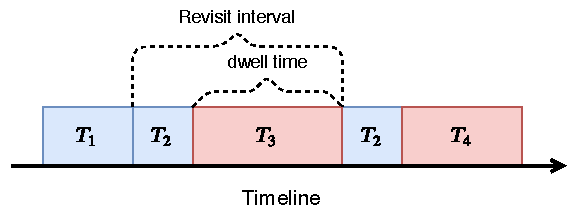
\includegraphics{figures/timeline.pdf}
    \caption{
        The looks for the tasks $T_i \forall i\in\{1,2,3,4\}$ are scheduled on a radar timeline. 
        The revisit interval and the dwell time of the looks are illustrated.
        The blue and red colors are used to indicate tasks corresponding to different radar functions such as tracking and search functions.
    }
    \label{fig:timeline}
\end{figure}

\subsection{Radar resource management techniques} \label{sec:RRM_tech}

\begin{figure}[tb]
    \centering
    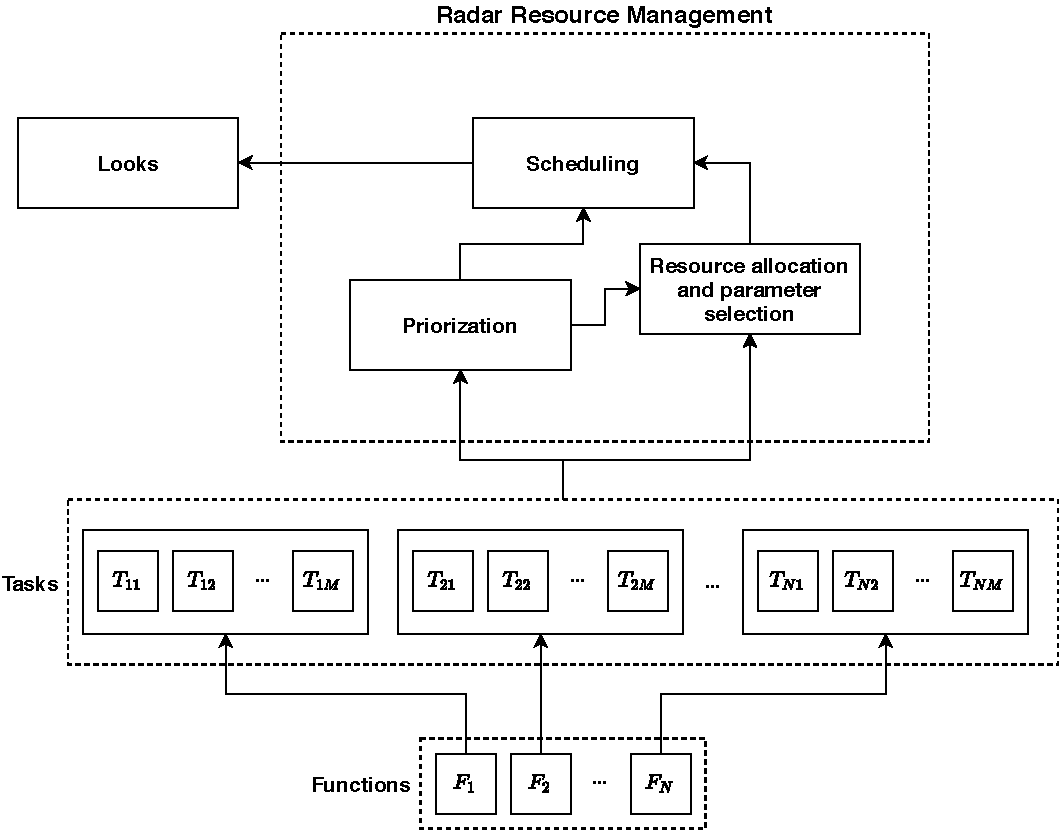
\includegraphics[width=.9\linewidth]{figures/RRM_diagram.pdf}
    \caption{Typical components in Radar Resource Management (RRM).}
    \label{fig:RRM_diagram}
\end{figure}

A typical RRM algorithm can be divided into three components that prioritize, allocate, and schedule radar resources, as shown in Figure \ref{fig:RRM_diagram}.
However, for some RRM techniques, the division is not strict.
For example, RRM techniques can implement jointly the functions of each aforementioned component while optimizing the objective function.
The following techniques for addressing RRM problems were identified in the literature \cite{Moo2016, Koch1999, Krishnamurthy2001, Wintenby2006, LaScala2006, Rajkumar1997, Rajkumar1998, Kastella1997, Kreucher2004, Kreucher2005, Xu2010}.

\begin{description}

\item[Rule-based approach.]

Rule-based RRM include approaches in which local objective is optimized instead of optimizing the global objective \cite{Koch1999}.
Alternatively, the parameters can be fixed, which could lead to allocating too little or too much radar resources for the radar tasks \cite{Hoffmann2014}.
Significant research direction in rule-based approaches is developing adaptive RIS algorithms \cite{Cohen1986, Gardner1988, Munu1992, ChengTing2007, Baek2010, Watson1993, Charlish2015, Keuk1975, Shin1995, Benoudnine2006}. Those algorithms will be covered in more detail in Section \ref{sec:tbm_ri}.


\item[Stochastic dynamic programming.]

Stochastic Dynamic Programming (SDP) is a generalized framework for solving decision-making problems under uncertainty \cite{Ross1983}. 
The Markov Decision Process (MDP) is a particular case of SDP for which the Markov property is satisfied, and the states and the actions are discrete \cite{Ross1983}.
The RRM problem can be interpreted as a decision-making problem in which the decision-maker needs to decide sequentially which radar task will be executed next, and how much radar resources are allocated for it \cite{Krishnamurthy2001, Wintenby2006, LaScala2006}.
An essential characteristic of the SDP approach is that the decisions are made to account for long-term consequences.
However, the optimal solution is unfeasible with realistic assumptions \cite{Wintenby2006}.
Therefore, the RRM is relaxed to a two time-scale RRM problem where the SDP is used to solve the slow-time-scale optimization problem and the low-level scheduler is responsible for solving the fast-time-scale scheduling problem \cite{Wintenby2006}.  


\item[Quality of service resource allocation model.] 

Quality of Service Resource Allocation Model (Q-RAM) was initially proposed in \cite{Rajkumar1997}.
Q-RAM algorithms optimize a global utility function while satisfying the resource constraints.
Thus, the approach is different from the rule-based RRM techniques in which local objectives are optimized.
Q-RAM addresses the resource allocation problem in which resources are allocated for the radar looks for a specific scheduling interval, but the actual order of the looks is not considered.
However, the schedulability requirement ensures that the looks can be scheduled when using a given low-level scheduling algorithm. 
In RRM problems that involve multiple resources, the Q-RAM optimization problem is unfeasible, but practical approximation algorithms are proposed in \cite{Rajkumar1998, Irci2010, Charlish2015a}.

\item[Information-theoretic approach.]

In the information-theoretic approach, the surveillance area is divided into grid cells \cite{Kastella1997, Kreucher2004, Kreucher2005, Xu2010}.
The probability of target existing in a given grid cell is calculated based on prior probabilities and past observations.
An information-theoretic measure is used to calculate the obtained utility for taking different actions i.e., selecting which cells to observe or which waveforms to use.
Thus, the information-theoretic approach does not differentiate search and tracking tasks since its purpose is to minimize uncertainty in the surveillance area.

\end{description}


\noindent
Some RRM algorithms have characteristics from multiple technique classes. 
For example, in \cite{Byrne2015, Byrne2016}, the objective function is similar to the Q-RAM approach but considers the long-term consequences as in the SDP approaches.
Additionally, in \cite{Esfahani2012}, locally optimized QoS parameters are utilized in allocating a radar time budget to optimize global objectives using a heuristic algorithm.

\subsection{Distributed MIMO radar transmitter-receiver selection}\label{sec:TX_RX_selection_review}

\begin{figure}[b]
    \centering
    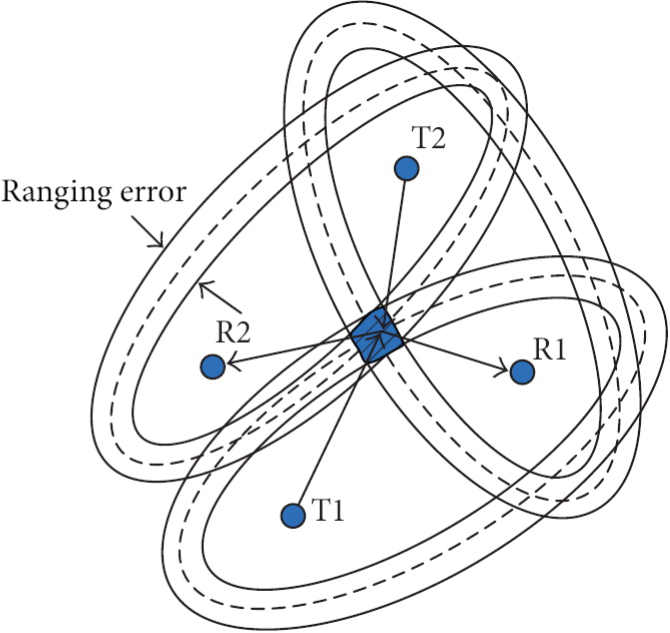
\includegraphics[width=0.5\textwidth]{figures/background/MIMO_TX_RX_selection.png}
    \caption{Target localization with distributed MIMO radar \cite{Sun2014}.}
    \label{fig:dist_MIMO_localization}
\end{figure}


In distributed MIMO radars, the increased number of channels provides additional spatial diversity and degrees of freedom at the cost of larger amounts of data to be processed as well as higher power consumption \cite{Haimovich2008}.
In addition, active TXs may expose their location, which might be undesired in specific applications.
Strategies for TX-RX subset selection are studied to obtain desired spatial diversity gain and reduce the cost and the power consumption simultaneously.

In \cite{Godrich2011a, Godrich2011}, the subset selection was formulated as a Knapsack
Problem (KP) which is a specific combinatorial optimization problem.
In the KP, each item in a given set of items are associated with a weight and a value, and the objective is to select such items that the total value is maximized while the total weight is below a certain limit.
However, in the considered KP formulations, the items were associated with costs instead of values such that total costs were minimized.
An item in the TX-RX subset selection problem is either a TX or a RX.

The KP in \cite{Godrich2011a} was formulated for minimal subset selection, in which a minimum number of TXs and RXs are selected with a required target localization accuracy.
Therefore, the weight in the KP formulation is a quantity related to the target localization uncertainty associated with a given subset, and the cost was the operational cost involved with using the subset of TXs and RXs.
In \cite{Godrich2011}, the KP was formulated for K-subset selection, in which the number of TXs and RXs in the subset is equal to $K$.
Therefore, the weight for each TX or RX is one, and the total weight is required to be less than $K$.
In addition, the cost was based on the target localization uncertainty.

The TX-RX subset selection strategies proposed in the literature utilize target localization accuracy related performance measures \cite{Godrich2011a, Godrich2011, Sun2014}.
The target localization accuracy is dependent on the geometry of a distributed MIMO radar layout, as depicted in Figure \ref{fig:dist_MIMO_localization}.
In \cite{Godrich2011a, Godrich2011}, Cram\`er-Rao Bound (CRB) was derived for the target position estimate, and a trace of the CRB was used as a performance measure.
The trace of the CRB is related to the Geometric Dilution Of Precision (GDOP), which is a commonly used measure in Global Positioning Systems (GPS) \cite{Sun2014}. 
An information-theoretic performance metric was proposed in \cite{Sun2014}.
This metric is called the Fisher Information Distance (FID). 
It calculates the similarity of target position probability distributions for measurements acquired with the TX-RX subset and the full set of TXs and RXs. 
The benefit of using FID is its ability to measure how close the subset performance is compared to the case where all TXs and RXs are selected \cite{Sun2014}.

There are multiple ways to solve the KPs mentioned earlier.
The most straightforward approach is to use exhaustive search as in \cite{Sun2014}.
However, the number of subsets grows exponentially as a function of the number of TXs and RXs.
Therefore, solving the problem may become intractable in the case of larger MIMO radar configurations.
In order to solve such a problem, heuristic approximation algorithms are proposed in \cite{Godrich2011a, Godrich2011} to optimize the KPs.
The algorithms are based on the following idea:
\begin{enumerate}
    \item Select all possible TX-RX pairs as initial subsets,
    \item Evaluate the performance measure for each subset augmented by one of the remaining TX or RX at a time, 
    \item For each subset, include the TX or the RX achieving the highest performance,
    \item Repeat steps 2 and 3 until the limit for the weights are exceeded, and
    \item Select the subset from the generated subsets that minimizes the total costs. 
\end{enumerate}
Such an algorithm is stated to achieve close to optimal performance with polynomial computational complexity \cite{Godrich2011a, Godrich2011}.

The target localization performance depends on the SNR and the TX-RX locations with respect to target locations, as discussed in \cite{Sun2014}.
Moreover, in \cite{Sun2014} it was found that the channels with a high SNR are typically chosen.
The SNR can be obtained, for example, by using equation \eqref{eq:radar_snr}, but it requires the target RCS to be known.
In \cite{Godrich2011a, Godrich2011, Sun2014}, it was assumed that the angle-dependent target RCS could be estimated from previous cycles for each TX-RX pair or the target RCS is initially known.
In general, the target RCS cannot be assumed known without estimating it. 
Thus, all the TX-RX pairs need to be probed regularly to ensure that the estimates are precise because the target is continuously moving, and the RCS might be dependent on the illumination and scattering angles.


\subsection{Adaptive revisit interval selection algorithms} \label{sec:tbm_ri}

An integral part of the Time Budget Management (TBM) is the selection of the Revisit Interval (RI) for the target tracking tasks.
The radar time resources can be released from tracking tasks by using longer RIs. 
However, the RI should be adjusted such that the tracking task can be maintained while minimizing the tracking load.
Short RIs should be used for maneuvering targets with high process noise to maintain the quality of state estimates at a tolerable level. 
Similarly, long RIs should be used for non-maneuvering targets with stable trajectories because the movement is more predictable.
Different adaptive Revisit Interval Selection (RIS) algorithms have been widely studied to release time resources from target tracking to other radar tasks \cite{Cohen1986, Gardner1988, Munu1992, ChengTing2007, Baek2010, Watson1993, Charlish2015, Keuk1975, Shin1995, Benoudnine2006}.
The algorithms are briefly covered in the following subsections.

\subsubsection{Residual-based algorithms}

Residual-based RIS algorithms adjust the RI adaptively based on the innovation sequence of the tracking filter.
These methods assume that the measurement data along each coordinate is decoupled so that the RI selection algorithm is executed for each coordinate in parallel, and the smallest RI selected.
In addition, range-rate measurements were not considered.
Therefore, innovation is written as a scalar value in the equations presented in this section.

In \cite{Cohen1986}, a novel RIS algorithm was introduced.
The RI $\ri$ was increased or decreased by using a simple recursive rule 
\begin{equation}\label{eq:update_resid}
    \ri(k) = \ri(k-1)\sqrt{\frac{\sigma_m}{|y_k|}},
\end{equation}
where $y_k$ is the innovation, and $\sigma_m$ is the standard deviation of the measurement noise.
The equation \eqref{eq:update_resid} was derived from the assumption that the prediction error at time instance $k$ is proportional to the acceleration and the square of the RI at time instance $k-1$.
For maintaining constant tracking error for maneuvering targets, the new RI needs to be proportional to the previous RI and inversely proportional to the square root of the change in acceleration.
However, the acceleration is unknown, but the change in acceleration is observed from the error in the innovation sequence.

The work in \cite{Cohen1986} was extended for $\alpha\beta\gamma$ filters \cite{Brookner1998} in \cite{Gardner1988}. 
The equation \eqref{eq:update_resid} was modified to use the cube-root instead of the square-root in the denominator.
Moreover, it was suggested that significant variations in $y_k$ could be smoothed by using a first-order low-pass filter.
The performance between $\alpha\beta$ and $\alpha\beta\gamma$ filters were compared in \cite{Munu1992}.
It was observed that $\alpha\beta\gamma$ filter could operate with longer update intervals than $\alpha\beta$ filter when the target is maneuvering.

A residual-based algorithm for the IMM estimator was proposed in \cite{ChengTing2007}.
The following equation was obtained for calculating the RI
\begin{equation}
    \ri(k) = \frac{4}{2^p}, \text{ } 4^p c < \frac{|y_s(k)|}{\sigma_m} < 4^{p+1}c
\end{equation}
in which $y_s(n)$ is the smoothed residual, and $c$ controls trade-off between the accuracy and the tracking load.
Furthermore, equation for $p$ can be written as
\begin{equation}
    p = \floor*{\log_4\frac{1}{c}|\frac{|y_s(k)|}{\sigma_m}|},
\end{equation}
where operator $\floor*{x}$ takes the highest integer less than or equal than $x$.
Also, the maximum RI was defined for the algorithm based on the used target motion models.

Baek \etal in \cite{Baek2010} proposed a residual-based algorithm for Kalman filters.
The algorithm was derived to keep the residual between the target position and the position estimate below the threshold $e_\text{th}$.
For the tracking filter, recursive equation to calculate revisit interval from previous revisit interval was obtained
\begin{equation}\label{eq:update_baek}
    \ri(k) = \ri(k - 1) \sqrt{\frac{e_0}{|y_k|}},
\end{equation}
where $e_0$ is the desired expected residual, which was derived from the measurement error covariance matrix, desired threshold $e_\text{th}$, and target priority.
A higher target priority implies that shorter RI is used to reduce the probability of target moving out from the threshold area defined by $e_\text{th}$.
The equations \eqref{eq:update_resid} and \eqref{eq:update_baek} are effectively the same if $e_0$ is replaced by $\sigma_m$.


\subsubsection{Error covariance matrix based algorithms}

\newcommand{\ndwells}{{n_d}}


The target position needs to be estimated \prior to steer the TX beam in the correct direction. 
The predictive error covariance matrix estimates the uncertainty in the predicted state variables.
Thus, it can be examined to evaluate the probability of the target being in the predicted position.
The predictive error covariance matrix is a function of RI because the state transition and process covariance matrices are a function of RI.
Thus, a criterion for the predictive error covariance matrix can be defined to formulate the RIS as an optimization problem.

Van Keuk proposed a criterion for an error covariance matrix in \cite{Keuk1975} that is widely utilized in the adaptive RIS literature.
In addition, an equation was proposed to calculate the RI efficiently for a target with a known or estimated Signer motion model \cite{RongLi2003} parameters.
Initially, the target tracking problem was considered in one-dimensional space such that the Van Keuk's criterion can be written as follows
\begin{equation}\label{eq:criterion}
    \sigma_p(t + \ri | t) \leq V_0 \sigma_m,
\end{equation}
where $\sigma_p(t + \ri | t)$ is the predicted standard deviation of the position error for time instance $t+\ri$ predicted from time instance $t$, $\sigma_m$ is the standard deviation of the measurement error, and the parameter $V_0$ is called track sharpness parameter.
In higher dimensions, $\sigma_p(t + \ri | t)$ is a square root of the maximum eigenvalue of the error matrix of the predicted position, and $\sigma_m$ is the standard deviation of the measurement error in the corresponding direction.
The RI was obtained as a solution for the following optimization problem
\begin{equation}\label{eq:van_keuk_optimization}
\begin{array}{ll}
     & \max_{\ri} \ri \\[7pt]
    \text{s.t. } &\sigma_p(t + \ri | t) \leq V_0 \sigma_m. 
\end{array}
\end{equation}
The approach assumed the Singer motion model with acceleration standard deviation parameter $\Sigma$ and correlation parameter $\Theta$.
Using the assumed models and steady-state Kalman filter equations, a heuristic rule to calculate $\ri$ was obtained
\begin{equation}\label{eq:keuk_time}
    \ri \approx 0.4 \left[ \frac{\sigma_m \sqrt{\Theta}}{\Sigma} \right]^{0.4} \frac{V_0^{2.4}}{1+\frac{1}{2}V_0^2}
\end{equation}
which approximately solves the optimization problem in equation \eqref{eq:van_keuk_optimization}.

The equation \eqref{eq:keuk_time} was proposed for calculating the RI efficiently, but the optimal value for the track sharpness parameter $V_0$ was not considered.
However, the work was extended in \cite{vanKeuk1993} to find suitable value for $V_0$ by considering the tracking load
\begin{equation}\label{eq:load}
    L = \frac{\E{\ndwells | \ri} \tau_d}{\ri}
\end{equation}
where $n_d$ is the number of dwells needed to obtain a successful detection, and $\tau_d$ is the dwell time.
It was assumed that only angular uncertainty needs to be considered when \eqref{eq:load} is minimized, 
because low uncertainty in the angle enables steering the beam in the correct direction.
Therefore, the criterion \eqref{eq:criterion} was reformulated by replacing the parameter $\sigma_m$ with the half-power beamwidth $B$ of the transmitted beam such that
\begin{equation} \label{eq:criterion2}
    \sigma_\angle(t + \ri | t) \leq V_0 B
\end{equation}
where $\sigma_\angle$ stands for the standard deviation of the error along the major axis of ellipsoid in the sine space \cite{vanKeuk1993}.
The sine space consists of $u$, $v$ and $d$ coordinates where $d$ is target range, $u=\cos \beta \sin \theta$ and $v=\sin \beta$ for elevation angle $\beta$ and azimuth angle $\theta$ \cite{Mailloux2017}.
The sine space is commonly used coordinate system with phased-array antennas.
A refined version of the RI rule was obtained based on the half-power beamwidth
\begin{equation}\label{eq:van_keuk_revisited}
    \ri \approx 0.4 \left[ \frac{\sigma_m d \sqrt{\Theta}}{\Sigma} \right]^{0.4} \frac{U^{2.4}}{1+\frac{1}{2}U^2}
\end{equation}
where $d$ is the target range, and $U$ is defined as
\begin{equation}
    U = \frac{V_0 B}{\sigma_m}.
\end{equation}
The optimization problem for $V_0$ was formulated as 
\begin{equation}
\begin{array}{ll}
     & \min_{V_0} \frac{\E{\ndwells | \ri} \tau_d}{\ri} \\ [7pt]
    \text{s.t.} & \sigma_\angle(t + \ri | t) = V_0 B
\end{array}
\end{equation}
where $\E{\ndwells | \ri}$ and $\ri$ are substituted with their closed-form expressions \cite{vanKeuk1993}.
In \cite{vanKeuk1993}, it was stated that fixed $V_0=0.3$ solves the optimization problem approximately with typical target parameters.

The research in \cite{Keuk1975, vanKeuk1993} was based on finding a formula to calculate the RI for the Singer motion model with known maneuver parameters.
However, in \cite{Shin1995} the work was extended to IMM estimators where the parameters of the Singer model were estimated online.
In other words, the parameters $\Theta$ and $\Sigma$ were calculated from the used IMM estimator models and their posterior mode probabilities.
Then, the equation \eqref{eq:van_keuk_revisited} was used to calculate the RI.

An optimal algorithm to maintain a desired state prediction error with IMM estimators was carried out in \cite{Watson1993}.
A threshold for the uncertainty was selected to be proportional to the measurement error covariance matrix.
Furthermore, the traces of the threshold matrix and the predicted covariance were set equal
\begin{equation}\label{eq:cov_th}
    \tr{ \vec{\Sigma}_{t+\ri|t} } = \tr{ \vec{\Sigma}_{\text{th}} },
\end{equation}
where $\vec{\Sigma}_{t+\ri|t}$ is the covariance of prediction error, and $\vec{\Sigma}_{\text{th}}$ is the threshold covariance matrix.
From equation \eqref{eq:cov_th}, a polynomial function is obtained which is a function of the RI $\ri$.
The non-linear optimization problem was solved in \cite{Watson1993} using Newton's method.

A practical algorithm to solve similar optimization problem as in equation \eqref{eq:van_keuk_optimization} for IMM estimators was proposed in \cite{Daeipour1994}. A finite set of RIs was defined, and a heuristic algorithm to select the revisit interval was proposed to avoid a computationally intensive optimization problem.
The algorithm is straightforward: the longest RI that satisfies the equation \eqref{eq:criterion2} was searched exhaustively by starting from the longest RI and then gradually decreasing it until the RI that satisfies the given criterion is found. 
The prediction equations of the IMM estimator are used for evaluating the equation \eqref{eq:criterion2}.

\subsubsection{Other algorithms}

The following algorithms do not directly correspond to any of the categories presented in the previous subsections.
However, the algorithms may simplify or extend the ideas of the RIS algorithms mentioned above.

 An IMM estimator with simple architecture and a fast algorithm for calculating the RI were proposed in \cite{Benoudnine2006}.
The IMM estimator was comprised of two models: a Constant Velocity (CV) model and a Constant Acceleration (CA) model.
The steady-state RIs were defined for the CV model $t_\text{CV}$ and for the CA model $t_\text{CA}$.
Then, the RI was obtained using a simple equation
\begin{equation}\label{eq:fimm}
    \ri = \mucv t_\text{CV} + \muca t_\text{CA},
\end{equation}
where $\mucv$ and $\muca$ are the probabilities for CV and CA models, respectively.

Another fast algorithm for RIS selection was also proposed in \cite{MasoumiGanjgah2017}.
An IMM estimator with three different maneuver models was used, and a minimum RI $\tmin$ and a maximum RI $\tmax$ were defined for the RIS algorithm.
The models were designed to have different maneuvering levels starting from low maneuvering model to high maneuvering model.
The RI was controlled recursively such that if the highest maneuvering model has the highest posterior probability, then RI is decreased by multiplying it with a constant less than one.
On the other hand, if the lowest maneuvering model has the highest posterior probability, then RI is increased by multiplying it with a constant higher than one.
Otherwise, the RI is kept the same as in the previous interval.
The algorithm resembles residual-based algorithms but uses a different control policy.

In \cite{Charlish2015}, it was shown that it may be beneficial to introduce anticipation for the RIS algorithms.
The anticipation was utilized to prevent significant prediction errors when the target moves through an occluded area.
The significant prediction errors can be prevented by acquiring high prediction accuracy by using short RIs before the target moves to the occluded area where the measurement accuracy is significantly reduced.
The RIS was formulated as a Partially Observable Markov Decision Process (POMDP) for which the immediate reward was defined as follows
\begin{equation}
    r = \frac{u\left(\vec{\Sigma}_{t+\ri|t} \right) \ri}{\tau_d},
\end{equation}
where $\tau_d$ is the dwell time, and the utility function $u(\cdot)$ is 1 if the prediction uncertainty is below a defined threshold.
If the prediction uncertainty is above the threshold, the utility function will gradually decrease towards zero.
The anticipation was obtained by maximising the discounted sum of rewards in equation \eqref{eq:discounted_sum}.

\subsection{Summary}

This chapter reviewed different RRM techniques and two specific RRM problems.
The adaptive rule-based RRM model is used for optimizing QoS performance for each radar task locally.
The other reviewed RRM models can improve performance by maximizing a global utility function.
However, those models require solving difficult optimization problems.

The TX-RX selection problem for distributed MIMO radars was presented.
Current solutions for the TX-RX selection problem were reviewed and their weaknesses were analyzed.
It was recognized that probing channels in distributed MIMO radars could be addressed with more sophisticated probing techniques.
Therefore, the TX-RX selection problem is addressed in Chapter \ref{sec:RL_TX_RX} by applying RL techniques.

Lastly, two distinct classes for RIS algorithms were identified. 
The classes were residual-based algorithms and error covariance based algorithms.
Moreover, most of the latest RIS algorithms for IMM estimators are error covariance based algorithms.
In Chapter \ref{sec:rl_ri}, principles of the RIS algorithms will be utilized to propose an RL approach for the RIS problem.


\newpage
\section{Reinforcement Learning Based Transmitter and Receiver Selection for Distributed MIMO Radars}\label{sec:RL_TX_RX}

Transmitter (TX) and receiver (RX) selection for distributed MIMO radars is studied to obtain the desired spatial diversity gain while reducing the data to be processed and the power consumption.
Previous studies in TX-RX selection for distributed MIMO radars assumed that the Signal-to-Interference-plus-Noise Ratio (SINR) is known \cite{Sun2014} or can be estimated \cite{Godrich2011a, Godrich2011}, as discussed in Section \ref{sec:TX_RX_selection_review}.
It is possible to estimate the SINR based on assumed particular propagation environments and target models, but a real-world radar environment may deviate from the assumed model and consequently lead to performance degradation.

Another way to form the estimates is to probe the different channels for a sufficient number of times to learn their state.
The probing needs to be efficient since the channels are continuously evolving, and the probing will impact the radar performance because it requires performing extra tasks in addition to the main operation of the radar.  Therefore, it is necessary to decide when to exploit the TX-RX subset currently providing the best payoff or explore other subsets that may or may not provide even higher SINR levels. 
This is the exploration-exploitation trade-off.

The Multi-Armed Bandit (MAB) framework provides policies for selecting actions to balance the exploration-exploitation trade-off while maximizing the employed reward function \cite{Lattimore2019}.
In the literature, such a framework is effectively used, for example, for opportunistic spectrum access, in which the secondary user must choose a frequency band in a way that does not cause interference to the primary user \cite{Zhao2008}.
Moreover, authors in \cite{Mukherjee2012} and \cite{Kuai2019} use a combinatorial MAB approach as a robust way for selecting the MIMO antenna subset for maximizing throughput in communication systems.
The combinatorial MAB formulation is used to address a problem with a large combinatorial action space.

In this chapter, a novel Reinforcement Learning (RL) based approach for the active TX-RX subset selection is proposed in the distributed MIMO radar context. 
It is based on the same principle proposed in \cite{Mukherjee2012} and \cite{Kuai2019}. 
However, the approach is generalized for index-based MAB algorithms and non-stationary environments. 
The generalized approach is simulated in a radar environment, and the performance of several different MAB algorithms is compared.

\subsection{Problem definition}

\newcommand{\ntx}{{N_{\text{tx}}}}
\newcommand{\nrx}{{N_{\text{rx}}}}
\newcommand{\srx}{{M_{\text{rx}}}}
\newcommand{\stx}{{M_{\text{tx}}}}


Assume a distributed MIMO radar system that consists of $\nrx$ receivers and $\ntx$ transmitters.
The radar system is constrained to use a subset of the TXs and the RXs at the same time to save resources such as power and reduce the probability of being detected by an adversary.
Each TX-RX pair is considered as a channel, and overall there are $\nrx\ntx$ channels.
The number of channels in a subset is $\srx \stx$, where both, the number of receivers $\srx$ and the number of transmitters $\stx$ in a subset are constrained with an equality constraint.
Selecting receiver $n \in \{1, 2, ..., \nrx\}$ and transmitter $m \in \{1,2, ..., \ntx\}$ is indicated with vectors $\vasvrx$ and $\vasvtx$ where
\begin{align}
    &\easvrx = 
    \left\{\begin{array}{l}
        1 \text{, when receiver $n$ is included in the set} \\
        0 \text{, otherwise}
    \end{array}\right.\\
    &\easvtx = 
    \left\{\begin{array}{l}
        1 \text{, when transmitter $m$ is included in the set} \\
        0 \text{, otherwise.}
    \end{array}\right.
\end{align}
Radar receivers are subject to both unintentional and intentional interference when observing target returns.
The quality of the received signal is typically characterized by the SINR.

In this thesis, the measured signal power $\esp$ at receiver $n$ from transmitter $m$ via the target is modeled as a stochastic process that may be non-stationary. 
The non-stationary character of $\esp$ can stem from the target moving in the environment, and 
the movement causes variability to path losses and the radar cross-section (RCS).
Moreover, unintentional and intentional interference levels might change in time, further contributing to the system's non-stationary behavior.
It is assumed that sufficiently accurate estimates of the noise power $\thnoise$ and the interference power $\eintnoise$ at receiver $n$ are available.
Therefore, the channel SINR can expressed on a linear scale as
\begin{equation}\label{eq:sinr}
     \esinrexp = \frac{\E{\esp} - (\thnoise + \eintnoise)}{\thnoise + \eintnoise },
\end{equation}
where the noise power and the interference power is subtracted from the received signal power and $\E{\esp} \geq \thnoise + \eintnoise$.
Note that the SINR is time-dependent because the distribution of the random variable $\esp$ varies in time. 


Performance in target detection and target localization depends on the SINR level \cite{Aittomäki2011, Godrich2011, Sun2014}.
Therefore, a reward function for RL is proposed that depends on vector $\vsinrexp$ that consists of all the SINR values $\esinrexp$.
The following reward function is used for the employed MAB learning
\begin{equation}\label{eq:reward_func}
    r(\vasvrx, \vasvtx | \vsinrexp) = \frac{1}{\srx \stx}\sum_{n=1}^\nrx \sum_{m=1}^\ntx  \easvrx \easvtx \esinrexp,
\end{equation}
which is a mean of SINR values for the selected channels on a linear scale.
Furthermore, the reward maximization problem can be formulated as
\begin{equation}\label{eq:obj_func}
    \begin{array}{ll}
                &   \max_{\vasvrx, \vasvtx} r(\vasvrx, \vasvtx | \vsinrexp) \\[7pt]
    \text{s.t.} &   
                \left\{\begin{array}{l}
                    \sum_{n=1}^N \easvrx = \srx \\
                    \sum_{m=1}^M \easvtx = \stx.
                \end{array}\right.
    \end{array}
\end{equation}
It is possible to find an optimal solution for the equation (\ref{eq:obj_func}) if $\vsinrexp$ is known.
However, $\vsinrexp$ is not known since we can only obtain the measurements $\esp$. 
Furthermore, it might not be possible to probe all the channels at the same time.
Therefore, $\vsinrexp$ needs to be estimated from the received signal. 
By probing the different channels, an estimate $\vsinrb$ of the channel SINR values can be formed.
An approximate solution for the objective (\ref{eq:obj_func}) is found when the estimate $\vsinrb$ is used to condition the reward function (\ref{eq:reward_func}).
Different subsets must be explored a sufficiently large number of times to reinforce the estimate $\vsinrb$ to identify the subset of TX-RX pairs yielding the highest SINR values.


\subsection{Multi-armed bandit formulation}

The stochastic MAB, introduced in Section \ref{sec:MAB}, have a finite set of arms and a single arm is selected at each time instant.
Therefore, the TX-RX selection problem in distributed MIMO radars could be formulated as follows.
An arm could be a subset of TX-RX pairs and the reward is calculated using the reward function \eqref{eq:reward_func}.
However, the number of the subsets is $\binom{\nrx}{\srx}\binom{\ntx}{\stx}$ which grows exponentially. This could make the problem unsolvable with the MAB approach because there is no time to explore all the arms in a given time horizon.
The amount of time available for learning the different channels depends on the dynamic nature of targets and the propagation scenario.
For example, if a target appears or disappears or does abrupt maneuvers, then rapid changes in the reward distributions will happen. 
On the other hand, smooth changes occur when a target moves on a smooth trajectory and gradually changes its orientation.

The exponentially increasing number of arms can be avoided by reformulating the MAB model so that each arm represents SINR for each channel and the agent can choose multiple arms at each time instant.
The arms are chosen to maximize the reward function and satisfy the constraints.
When this formulation is used, the Q-values introduced in Section~\ref{sec:MAB} are the channel SINR estimates $\vsinrb$.
The total number of arms is reduced to $\nrx\ntx$ and the agent selects $\srx\stx$ arms at each iteration.
The formulation is known as the combinatorial MAB, in which the subset of arms is called a super arm \cite{Chen2014}.
The reformulation is possible because the reward function ($\ref{eq:obj_func}$) is an increasing function of the radar channel SINR values and each arm is independent since waveforms from different transmitters do not interfere with each other if orthogonal waveforms are used.

Usually, in the combinatorial MAB problem, the agent does not know the mapping from the arm rewards to the super arm rewards.
However, the reward function $\eqref{eq:reward_func}$ is known, which enables using the MAB algorithms from the classical MAB problem.
Authors in \cite{Mukherjee2012} and \cite{Kuai2019} use a similar approach for MIMO antenna selection in mobile communications to maximize throughput.
The approach in \cite{Mukherjee2012} uses the UCB1 algorithm and the reward statistics are constant, while authors in \cite{Kuai2019} use Thompson sampling, and both non-stationary, as well as stationary rewards, are considered.

In this study, the approaches in \cite{Mukherjee2012} and \cite{Kuai2019} are generalized for any index-based MAB algorithm, described in Section \ref{sec:MAB}, and non-stationary reward distributions.
The proposed algorithm for solving the combinatorial MAB problem with a known mapping from the arm rewards to the super arm rewards is shown in Algorithm~\ref{alg:gcmab}.
On line~\ref{alg:calc_idx} of the Algorithm~\ref{alg:gcmab} any index-based MAB algorithm can be used to find the indexes, and on line~\ref{alg:find_sa} any optimization method can be used to find the super arm.
The indexes calculated by a MAB algorithm will ensure that the exploration-exploitation trade-off is balanced well.

The principles of the Algorithm~\ref{alg:gcmab} can also be applied for \egreedy policy by using the SINR estimates $\vsinrb$ instead of the indexes.
Moreover, different subsets are explored by selecting them randomly.
However, the exploration is not as efficient as with index-based policies, because the fact that the super arm rewards are a function of the arm rewards is not utilized.

\begin{algorithm}[h]
\SetAlgoLined
\While{not end of the time horizon}{
calculate indexes for all arms\; \label{alg:calc_idx}
find the super arm using the indexes\; \label{alg:find_sa}
pull the super arm\;
\If {non-stationary rewards}{
discount rewards for all arms\;
discount exploration parameters for all arms\;
}
observe the arm rewards\;
update the arm rewards\; 
update the exploration parameters\;
}
\caption{Proposed generalized algorithm}
\label{alg:gcmab}
\end{algorithm}

\subsection{Numerical examples}
\label{sec:sim}


\subsubsection{System configuration}
\label{sec:sys_conf}
The simulated MIMO radar system consists of $\nrx=6$ receivers and $\ntx=4$ transmitters.
A subset with $\srx=3$ receivers and $\stx=2$ transmitters is selected, so that six out of 24 possible channels are used at any time instance.
It is possible to use an exhaustive search to find the super arm because there are only 120 different subsets.
The simulation environment is visualized in Figure \ref{fig:env}.

\subsubsection{Scattering model}
\label{sec:sc_model}

The target illumination angle and the scattering angle are usually different for each TX-RX pair in distributed MIMO radars.
Therefore, the RCS model depends on the angles to the receiver and the transmitter.
The dependency on the angles for receiver $n$ and transmitter $m$ is denoted by $\ercs$ which is a product between two scattering coefficients taken from the monostatic target RCS model at the illumination angle and the scattering angle.
The simplistic monostatic RCS model used in simulations is expressed by a simple sum of cosine functions $0.064 \cdot \abs{2.5\cos(\phi) + 7\cos(2\phi) + 3\cos(3\phi) + 3\cos(4\phi)}$, where $\phi$ is the backscatter angle.

The target RCS fluctuation is modeled based on the Swerling I model.
Hence, the power loss of the target fluctuation $c$ is modeled by the exponential distribution with the scale parameter equal to one, and $c$ remains constant between two subsequent time instances.

\subsubsection{Propagation environment model}
\label{sec:env_model}

The environment model includes path losses, thermal noise, and external interference.
The path loss $\epl = d_\text{tx}^{-2} d_\text{rx}^{-2}$ is a product between
reciprocal of target's squared distance to the transmitter and the receiver.
The thermal noise power $\thnoise=0.001$ is constant in time and the same for all the channels.
Also, the interference power $\vintnoise=[0.1, 0.9, 0.3, 0.1, 0.2, 0.4]^T$ is constant in time and $\eintnoise$ is the interference power at receiver~$n$.

\begin{figure}[!tb]
    \centering
    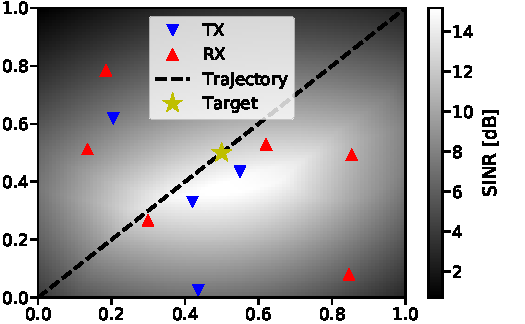
\includegraphics[width=.6\textwidth]{figures/MAB/env.pdf}
    \caption{Simulation setup.
    The target position is shown for the stationary case and the trajectory for the non-stationary case. 
    The heat map indicates the mean channel SINR at every position when the target scattering coefficient is excluded and all the channels are active.}
    \label{fig:env}
\end{figure}

\subsubsection{Reward distribution}

The agent aims to find the super arm with the highest reward based on the equation \eqref{eq:reward_func}. 
To create the arm rewards, we define an instantaneous SINR measure $\esinr$ that satisfies $\E{\esinr} = \esinrexp$ where $\esinrexp$ is the channel SINR. 
The value $\esinr$ is calculated using the equation \eqref{eq:sinr}, where the expectation is replaced with the power measurement $\esp$. 
To simplify the simulations, 
the target scattering coefficient $c$ remains constant through a single measurement period, and the stochasticity of the noise and the interference powers in the measurements are approximated to be negligible. 
Therefore, the rewards for each arm are simulated by
\begin{equation}
    \esinr  \sim \text{Exp}\left(\esinrexp\right),
\end{equation}
which is the exponential distribution with mean of $\esinrexp$.
The channel SINR $\esinrexp$ on a linear scale for receiver $n$ and transmitter $m$ is calculated from the models defined in Sections \ref{sec:sys_conf}, \ref{sec:sc_model}, and \ref{sec:env_model} as follows
\begin{equation}
    \esinrexp = \frac{\epl \ercs \epower}{\thnoise + \eintnoise},
\end{equation}
where the transmit power $\epower=1$ is constant in time and equal for each transmitter.


\begin{figure}[!tb]\centering
    \subfloat[Stationary case.]
    {
        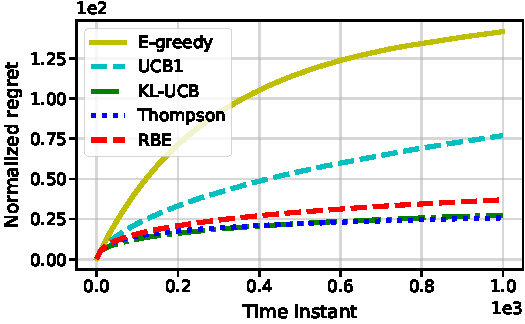
\includegraphics[width=.45\textwidth]{figures/MAB/stationary/cmab/regret.pdf}
        \label{fig:stationary_regret}
    }
    \hfill
    \subfloat[Non-stationary case.]
    {
        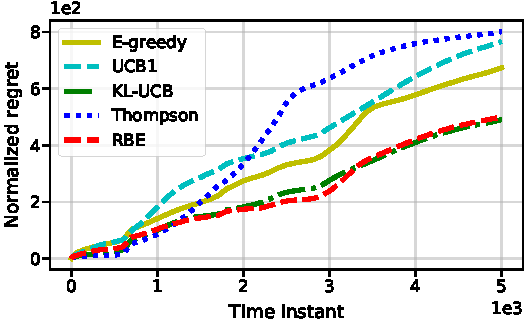
\includegraphics[width=.45\textwidth]{figures/MAB/non_stationary/regret.pdf}
        \label{fig:non_stationary_regret}
    }
    \caption{The normalized regret at each time instant. 
            RBE and KL-UCB perfom well in the both cases.}
    \label{fig:regret}
\end{figure}

\begin{figure}[!tb]\centering
    \subfloat[Stationary case.]
    {
        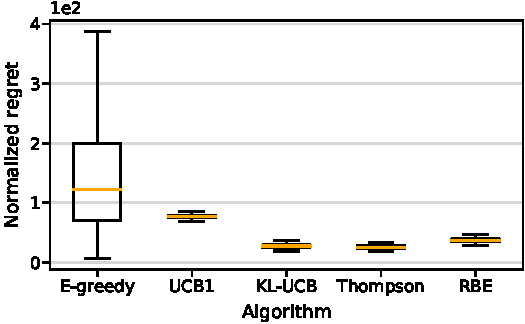
\includegraphics[width=.45\textwidth]{figures/MAB/stationary/cmab/regret_box.pdf}
        \label{fig:stationary_ci}
    }
    \hfill
    \subfloat[Non-stationary case.]
    {
        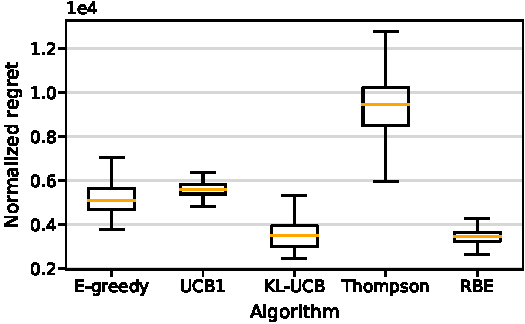
\includegraphics[width=.45\textwidth]{figures/MAB/non_stationary/regret_box.pdf}
        \label{fig:non_stationary_ci}
    }
    \caption{The normalized regret for the whole time horizon compared between different simulation runs.
            RBE and KL-UCB obtain excellent results in both stationary and non-stationary scenarios.}
    \label{fig:ci}
\end{figure}

\begin{figure}[!tb]
    \subfloat[Stationary case.]
    {
        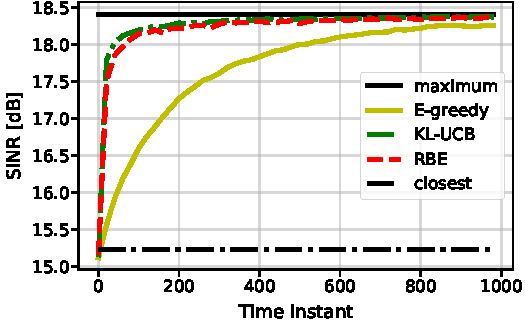
\includegraphics[width=.45\textwidth]{figures/MAB/stationary/cmab/sinr.pdf}
        \label{fig:stationary_sinr}
    }
    \hfill
    \subfloat[Non-stationary case.]
    {
        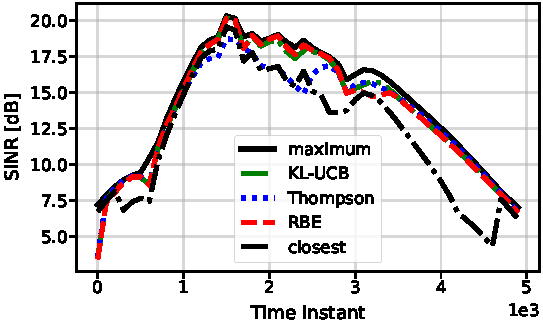
\includegraphics[width=.45\textwidth]{figures/MAB/non_stationary/sinr.pdf}
        \label{fig:non_stationary_sinr}
    }
    \caption{Reward at each time instant.
    The reward is a mean of the channel SINRs in a linear scale for the selected subset.
    The MAB algorithms are compared to a simple exploration-free method in which the subset of the receivers and the transmitters closest to the target is selected.
    On average, most of the MAB algorithms obtain rewards close to the maximum rewards.}
    \label{fig:sinr}
\end{figure}

\subsection{Simulation results}

Two different scenarios are studied in the simulation examples. 
In the stationary scenario, there is a target that remains stationary at position $(0.5, 0.5)$.
In the non-stationary scenario, a target moves from $(0, 0)$ to $(1, 1)$ on a linear trajectory with a constant velocity.
All other parameters for the environment remain the same in both scenarios.
The five algorithms that were briefly reviewed in Section~\ref{sec:MAB} are used in the simulations.
In addition, a simple method that selects the closest subset at each time instant is used to compare the MAB algorithms to a more conventional exploration-free method. 
The performance of the different MAB algorithms was evaluated using Monte Carlo simulations with $1000$ iterations.

The MAB algorithms are compared between each other in terms of normalized regret given by the equation \eqref{eq:reg}. 
The normalized regret through the simulation period is shown in Figure~\ref{fig:regret}.
Also, box plots of the regrets are shown in Figure~\ref{fig:ci}.
The comparison between the exploration-free method and MAB algorithms is performed by comparing the expectation of the achieved rewards through the simulation period.
The achieved rewards for two well-functioning MAB algorithms, 
the worst MAB algorithm and the exploration-free method are shown in Figure~\ref{fig:sinr}.
The overall results show that the MAB algorithms improve the performance through the time horizon and outperform the exploration-free method in stationary and non-stationary cases.
Moreover, the RBE algorithm stands out with excellent reliability and regret performance in both cases.

\subsubsection{Stationary target}

In the stationary case, the learning rate can be set to $\alpha=n(a)^{-1}$, as discussed in Section \ref{sec:MAB}.
The value of $\epsilon$ for $\epsilon$-greedy exploration is set to 0.1, which means that it explores random subsets 10\% of the time.
Lower $\epsilon$ can sometimes result in lower regret, but the variance of the regret may increase.
The value 0.1 was found empirically in this simulation.
The other algorithms do not have any tunable parameters.
The time horizon is set to 1000, which is sufficiently long for finding the optimal TX-RX configuration.

The stationary target implies that the expected rewards of the arms do not change in time.
Therefore, it is possible to achieve a logarithmic regret \cite{Lattimore2019}.
From Figure~\ref{fig:stationary_regret}, it can be observed that all algorithms other than $\epsilon$-greedy can achieve sublinear regret.
Algorithms like Thompson sampling and KL-UCB, which require knowledge about the reward distribution, have excellent performance in these simulations.
The $\epsilon$-greedy algorithm has the highest regret, and it is visible in Figure~\ref{fig:stationary_ci} that such random policies have a high variance.
Algorithms with higher variance make the learning less reliable even though they can some times find the optimal action faster than more reliable algorithms.

Figure~\ref{fig:stationary_sinr} visualizes the expected rewards at each time instant.
The main difference between the MAB algorithms is the time taken to find the optimal super arm.
The gap between the maximum expected reward and the obtained expected rewards will decrease as a function of time for algorithms that achieve sublinear regret.
Therefore, $\epsilon$-greedy with constant exploration probability will eventually have an approximately constant gap between the maximum expected rewards and the obtained expected rewards.
It can be observed that the MAB algorithms perform much better than the exploration-free method.

\subsubsection{Non-stationary target}

The algorithms adapt to the non-stationary conditions by using the constant learning rate used to discount the Q-values and the exploration parameters.
Thus, the learning rate is set to $\alpha = 0.998$.
Also, each element of $\vsinrb$ is divided by the maximum value before calculating the index.
This ensures that enough exploration is done at each time instant even if the scale of the rewards changes over time.
The value of $\epsilon$ for $\epsilon$-greedy algorithm is kept at 0.1.
The asymptotic optimality cannot be achieved since the exploration bonus will never vanish completely.
However, the considered algorithms have differences in their exploration efficiencies, as can be observed from the different regrets in Figure~\ref{fig:non_stationary_regret}.

In Figure~\ref{fig:non_stationary_regret}, it can be seen that KL-UCB and RBE achieve the lowest regret in the non-stationary case.
Thompson sampling does not adapt well for the non-stationary case even if it performed quite well in the stationary case.
The $\epsilon$-greedy algorithm has lower regret than Thompson sampling but it still performs worse than the other algorithms. 
The Figure~\ref{fig:non_stationary_ci} demonstrates that the RBE algorithm has a minimal regret with low variance.
Also, the median performance is better than with any other of the used algorithms.
Hence it is a promising algorithm for the radar problem at hand. 
The other algorithms which performed well in stationary reward scenario have poorer performance in non-stationary reward case.
The changes in reward distributions will force the agent to switch the arm if the Q-value for the arm under exploitation becomes lower than the other Q-values.
Therefore, in the case of a non-stationary target, the $\epsilon$-greedy algorithm achieves a smaller variance on regret than with stationary targets.

The achieved rewards are compared in Figure~\ref{fig:non_stationary_sinr}.
All MAB algorithms perform on average better than the exploration-free method through the whole simulation period.
Also, it is visible that the mean SINR of the MAB algorithms is close to the optimal at most of the time instances. 
Moreover, the performance gap between MAB algorithms is not as significant as in the stationary scenario.

\subsection{Summary}
\label{sec:tx_rx_summary}

The transmitter-receiver subset selection problem, in which the channel SINR values are unknown, was considered for the distributed MIMO radars.
Since only a subset of the channels can be selected simultaneously, it was shown that such problems have to deal with the exploration-exploitation trade-off to identify the optimal subset without degrading the radar performance.
The problem was formulated as the combinatorial multi-armed bandit problem, and a reinforcement learning algorithm was proposed to solve the problem.
It was shown that reinforcement learning could be effectively used to continuously improve the subset selections and outperform the proposed exploration-free method.



\newpage
\section{Reinforcement Learning Approach for Revisit Interval Selection}\label{sec:rl_ri}

An essential Radar Resource Management (RRM) problem in multifunction radars is to determine how to allocate and schedule the limited time budget among the different radar tasks. 
This problem is called the Time Budget Management (TBM) problem, as discussed in Chapter \ref{sec:existing_RRM}.
Electronically steerable antennas used in modern radars provide flexibility to execute radar tasks in an arbitrary order because steering the radar beam takes an insignificant duration of time. 
Therefore, TBM algorithms are studied to exploit the flexibility in controlling the radar beam.
In this chapter, a Reinforcement Learning (RL) method is proposed to address the TBM problem.

In Section \ref{sec:RRM_tech}, different techniques for RRM were introduced.
For RL methods, addressing the TBM problem with the Stochastic Dynamic Programming (SDP) technique seems appealing because the RL algorithms are used to solve MDPs.
However, applying RL algorithms to find even an approximate solution can be challenging because of two reasons:
\begin{enumerate}
    \item number of targets can change in time, and
    \item the TBM problem is a Partially Observable Markov Decision Process (POMDP).
\end{enumerate}
The first difficulty affects the dimensions of the state and the action spaces. 
For example, in multi-target tracking, the observation could be a combination of belief states of each target, and the action could be to choose which tracks will be updated next.
In that case, the number of actions would depend on the number of targets, and if an observation is presented as a matrix, the dimension of the matrix would depend on the number of targets.
Discretizing the observations would not help either since the number of discrete observations would grow exponentially as the number of targets increases.

The second difficulty is related to a more general problem with sensing systems; the variables derived from the radar measurements always include a certain degree of uncertainty.
However, there are at least a few different ways to tackle the POMDP problems using RL.
For example, a Markov Decision Process (MDP) state can be approximated from a finite length sequence of past observations, or a model could be used to extract the belief state.
The former approach can be implemented by stacking observations to approximate a state as in \cite{Mnih2013}, or by using recurrent neural networks as in \cite{Hausknecht2015}.
The downside is that typically such approaches require a large amount of training.
In the latter approach, the RL policy depends on the model.
Thus, modeling errors can decrease the performance of the policy.
In radar applications, however, the latter method is still attractive since typically, the required models already exist, and training can be faster compared to the former approach.

To avoid the difficulty with the variable number of targets, an optimal TBM problem is relaxed to a more manageable problem using a RRM technique that was presented in Section \ref{sec:RRM_tech}.
The TBM problem is addressed with a rule-based approach, in which an adaptive Revisit Interval Selection (RIS) algorithm can be used to select the Revisit Interval (RI) for each tracking task.
This approach enables using the RL policy for each track separately, thus making the actions and observations easier to present.

The proposed RL formulation is assuming a Single Target Tracking (STT) scenario. 
Therefore, the formulation is not addressing the track association and implementation of the low-level scheduler.
However, the RL approach is extendable to Multi-Target Tracking (MTT) scenarios by using a low-level scheduler, and by considering the probability of mixing tracks with providing relevant observations for the RL agent.
In the STT scenario, it is possible to experiment if the learning-based approach can help to tackle problems caused by modeling errors that affect conventional non-learning-based algorithms.
The performance of the RL approach is investigated in Monte Carlo simulations by evaluating the Probability to Lose a Track (PLT) and the tracking load.

In the following sections, an RL approach is proposed for the RIS problem and evaluated using Monte Carlo simulations.
Section \ref{sec:system_description} describes the considered radar systems.
In Section \ref{sec:RL_formulation}, the RL formulation of the RIS problem is proposed for the radar system introduced in Section \ref{sec:system_description}.
Section \ref{sec:ri_setup} gives numerical examples that are used to evaluate the RL approach in Monte Carlo simulations. 
Lastly, Section \ref{sec:ri_sim} presents the simulation results.


\subsection{Assumed radar system} \label{sec:system_description}

The actions, observations, and rewards of the RL formulation depend on the radar system for which the RL algorithm is applied.
Notably, the system dictates the available information to be used as the rewards and the states, and it designates the possible actions the radar system can take.
 
The assumed radar system searches new targets using the search function. 
A track is initiated for a target before entering the tracking loop. 
In the assumed radar system, the tracking loop is implemented by the following steps.


\begin{enumerate}
\item\textbf{Predict the target position at the current time instant denoted as $t_k$.}

The target position is predicted using a tracking filter. The prediction is implemented by propagating the predictive tracking equations with an processing interval $\dt$. 
Therefore, the RI $t_r$ is equal to $\dt$ multiplied by an arbitrary positive integer.

\item\textbf{Illuminate target at the predicted position.}

The center of the beamlobe is directed to the predicted target position. 
The center beam SNR is assumed to be a constant quantity $SN_0$ if the predicted angle is precisely the target angle. 
On the other hand, if an angle error exists, the SNR will degrade depending on the transmit beamshape. 
In a real-world radar, the center beam SNR could be kept approximately constant by adaptively controlling the transmit power using, for example, the equation \eqref{eq:radar_snr} and the estimated target range. 
Another way to control the SNR is to use different integration times but controlling it would add another dimension to the TBM problem. 
Therefore, a constant integration time is assumed here.

\item\textbf{If the target was detected, update the state estimate. If no detection obtained, either return to step 1 if the number subsequent dwells is below a threshold $\nmax$ or otherwise flag the target lost and exit the tracking loop.}

In the latter case, the target is considered lost, and it is not required to address here how the radar responds to such a scenario. 
In some radars, the track could be kept in memory waiting for the scenario where the target is found again, for example, by the search function. 
Then, the tracking loop could be restarted.


\item\textbf{Select the RI $\ri$.}

The RI is selected by using a RIS algorithm.
For example, RIS algorithms reviewed in Section \ref{sec:tbm_ri} could be used, or the RI could be selected by an RL agent described in Section \ref{sec:RL_formulation}.

\item\textbf{Return to step 1 before time instant $t_k + \ri$.}

The uncertainty in the predicted state estimates will grow as a function of time. Therefore, $t_k + \ri$ is the deadline for updating the track, but the update can be done before the deadline depending on the implementation of the resource manager.

\end{enumerate}

The track loop would be the same for each target in the MTT scenario. 
However, in the assumed STT tracking scenario, only one tracking loop can occur. 
The STT scenario simplifies the RIS problem because the track association is not needed to consider.


\subsection{Reinforcement learning formulation}\label{sec:RL_formulation}

The RL formulation is proposed for RL algorithms with discrete action and state spaces. 
Especially, the Q-learning algorithm is used in this study. 
Section \ref{sec:actions} proposes two different action spaces.
Then, Section \ref{sec:rewards} proposes a reward function that reduces the risk of losing tracks while minimizing the tracking load. 
Lastly, in Section \ref{sec:states} various discrete state spaces are introduced for the RIS problem.

\subsubsection{Actions} \label{sec:actions}

The RL agent could control the RI using two different approaches.
One approach is to select the RI from a set of intervals.
This approach will be called direct selection.
The other approach either decreases or increases the RI with some delta value, so this approach is called delta selection.
In other words, the action is mathematically interpreted as follows
\begin{equation}
    \ri(k) = \left\{
        \begin{array}{l l}
            A_k & \text{if direct selection used} \\
            \ri(k-1) + A_k &  \text{if delta selection used}
        \end{array}\right.
\end{equation}
where $A_k$ is the action taken at time instance $k$, and $\ri(k)$ is the RI selected at time instance $k$.
Both approaches can have either a continuous or a discrete action space.
Furthermore, the discrete action space is just a discretized version of the continuous action space $A_k \in [\amin, \amax]$.

The action space for direct selection is discretized, such that resulting RIs are equally spaced.
The minimum RI $\tmin=\amin$ and the maximum RI $\tmax=\amax$ need to be loosely defined for the approach. 
Loosely defining means that $\tmin$ can be shorter RI than the radar may use and similarly $\tmax$ can be longer.
For example, the equation \eqref{eq:van_keuk_revisited} could be used or different values could be examined in simulations. 

An example set of actions for direct selection is $A_k \in \{0.5, 1.0, 1.5, 2.0, 2.5\}$, where $\tmin=0.5$ and $\tmax=2.5$, and size of the action space is $5$.
In general form, the action space for direct selection is defined as follows
\begin{equation}\label{eq:as_direct}
    \Asdir \coloneqq \{ \frac{n \tmax + (\nacts-n-1) \tmin}{\nacts-1} \}_{n=0}^{\nacts-1},    
\end{equation}
where $\nacts$ is the size of the action space.
Lower $\nacts$ enables faster learning since there are fewer actions to be explored.
However, larger $\nacts$ may enable higher performance since a larger variety of RIs can be used.

The action space for delta selection is defined using an equal number of decreasing and increasing delta values. 
In addition, the action $a=0$ is included that neither increases nor decreases the RI.
The deltas are spaced with uniform distances as in \eqref{eq:as_direct}.
The maximum action $\amax=\deltalim$ and minimum action $\amin=-\deltalim$ are defined using the parameter $\deltalim$ which should be chosen along with the parameter $\nacts$ to achieve sufficiently large deltas with a satisfactory resolution.
An action space for delta selection could be for example $\{ -1.0, -0.5, 0, 0.5, 1.0 \}$, where $\deltalim=1$ and $\nacts=5$.
The general form of delta selection action space is
\begin{equation}\label{eq:as_delta}
    \Asdelta \coloneqq \{ \frac{\deltalim \left( 2 n - \nacts + 1 \right)}{\nacts-1} \}_{n=0}^{\nacts-1},
\end{equation}
where $\nacts$ should be a positive odd number.
Contrary to the direct selection, there are no hard upper or lower limits for the RI other than the limits given by the radar system.
In addition, $\deltalim$ can be much lower than $\tmax - \tmin$.
However, achieving the desired RI might take multiple actions, where the number of actions required depends on $\deltalim$ and $\nacts$.

\subsubsection{Reward} \label{sec:rewards}

The agent's overall objective is to minimize the time budget needed to maintain a track and prevent track losses based on the cost of losing a track.
The objective should be reflected in the immediate or cumulative rewards given for the RL agent, as shown in equation \eqref{eq:discounted_sum}. 
The proposed immediate rewards are based on the tracking load in equation \eqref{eq:load} and the cost of losing a track as follows
\begin{equation}
    r = \left\{
    \begin{array}{ll}
        -\closs & \text{if target lost} \\
        -\frac{n_d}{\ri} \tau_d & \text{otherwise},
    \end{array} \right.
\end{equation}
where $\tau_d$ is the dwell time and $n_d$ is number of dwells needed to achieve a detection, and $\closs$ is the cost of losing a track.
The penalty $\frac{n_d}{\ri}\tau_d$ is the tracking load in equation \eqref{eq:load} without expectation on the number of dwells, and it is referred to as temporal tracking load.
The discount factor $\lambda$ can be used to control how much the future tracking load and the possibility to lose a track are valued.
The agent can trade the immediate performance for better long-term performance when $\lambda > 0$.
However, when $\lambda = 0$, the policy may converge faster.

The value for $\closs$ can be selected using a heuristic design rule based on a simplified MDP with two states.
The states of the MDP represent if a target is lost or not.
An agent needs to select an action from two competing actions.
One of the actions, denoted as $a_1$, will have a tracking load of $\lref$, and when taking it, the track can not be lost.
For the other action, the track is lost with probability $1$, and the action is denoted as $a_2$.
If the tracking load $\lref$ is equally bad as losing a track, the parameter $\closs$ should be defined such that
\begin{equation}\label{eq:closs_criterion}
    \sum_{i=0}^\infty \lambda^i \lref = \closs
\end{equation}
which indicates that the discounted sum of rewards when always taking action $a_1$ should be equal to the penalty of losing track if action $a_2$ is taken.
Equation \eqref{eq:closs_criterion} can be rewritten into form
\begin{equation}
    \closs = \frac{1}{1-\lambda} \lref
\end{equation}
 by using the geometric series.

To understand the rewards in more detail, their expected values are examined.
The expected value of an immediate reward given the state $s$ and action $a$ is
\begin{equation}\label{eq:exp_reward}
    \E{R_{t+1} | S_t=s, A_t=a} = -(1-\ploss(s, \ri)) 
        \frac
        {
            \mathbb{E} \left[ n_d | s, \ri \right]
        }
        {
        \ri
        } 
        - \ploss(s, \ri) \closs
\end{equation}
where $\ploss(s, \ri)$ is the probability to lose a target when in state $s$ and using the RI $\ri$, and $\E{n_d|s, \ri}$ is expected value of the number of dwells.
Equation \eqref{eq:exp_reward} is also the action-value in myopic case.
The non-myopic action-value is more complicated since the MDP can transition to the terminal state if the target is lost.
Therefore, 
\begin{align}
    \E{\sum_{i=0}^\infty \lambda^i R_{t+1} | S_t=s, A_t=a} =& \E{R_{t+1} | S_t=s, A_t=a} + (1-\ploss(s, \ri)) \lambda \\
    & \sum_{s'\in \Ss} p(S_{k+1}=s'|S_{k}=s, A_{k}=a)  V(s')  
\end{align}
where $(1-\ploss(s, \ri))$ shows that the non-myopic part is weighted by the probability of not losing a target.

\subsubsection{States and observations} \label{sec:states}


The observations obtained by the agent are critical since those are the only source of information for the agent to distinguish in which situation it is currently acting.
In RL, observation is generally a partial observation of an environment state.
The environment state describes all the information that is needed to determine how the environment responds to an action of the agent. 
An observation or sequence of observations is denoted as an agent state.
The agent state contains the information that is available and relevant for the agent to choose an action.
Moreover, the achievable quality of the policy depends on the amount of available information.
For the Q-learning algorithm, the agent state needs to be discrete and approximately Markovian.

The information from the radar system is typically provided by continuous variables, and therefore, discretization is required.
The state is obtained by discretizing the continuous values into bins of equal sizes with bin edges given by
\begin{equation}\label{eq:state_limits}
    \frac{\ghigh - \glow}{N_d - 2} n + \glow,
\end{equation}
where $N_d-2$ is number of the bins, $n \in \{0, 1, ..., N_d-2\}$ is the index of the edge, and
the values $\glow$ and $\ghigh$ define the lower and the upper limits for the bin edges.
Two states are defined for the continuous values below $\glow$ and above $\ghigh$, such that $N_d$ discrete states are obtained in total.
In some cases, the required Markov property can be approximately satisfied by using a subset of past actions and observations \cite{Mnih2013}, but for discrete states, the cardinality of the state space will grow exponentially.


In the RIS problem, 
the environment state includes, for example, the target kinematic state and the corresponding belief state obtained by the tracker. 
The belief state and any signals from the radar can be used as an agent state, but only important information needs to be extracted to prevent the exponentially growing number of states. 
One good source of information from the tracking filters is the innovation sequence. 
It includes information about how well the tracker predicted the target position compared to the position measurement. 
In addition, range-rate can be examined in radars with Doppler capability. 
The simplest way to utilize the innovation sequence in discrete RL algorithms is to use the most recent innovation as a state. 
The size of the state space can be further reduced by using only the innovation in the target position's angle, assuming that the target range is less critical for steering the radar beam in the correct direction.
The state is not fully Markovian since the angle estimates contain noise. 

Another appealing option is to use the mode probabilities $\modeprob$ as a state if the tracking filter is a multiple model estimator such as the Interactive Multiple Model (IMM) estimator. 
The number of discrete states remains manageable as long as the number of the discrete mode probabilities and the modes remains sufficiently low. 
A more conventional RIS algorithm that obtains the RI using the mode probabilities was presented in equation \eqref{eq:fimm}.

The state spaces based on the innovation or the mode probabilities can be further extended by augmenting the previous RI to the state presentation.
Also, two additional states are included in the state space. 
One is for a lost target and the other for a track initiation.
The latter state enables the agent to learn to select RI at the beginning of the tracking task, where the tracking filter might have unreliable estimates.
The number of discrete states is $N_s = 2+N_d$ if the previous RI is not included into state and $N_s = N_d N_a + 2$ otherwise.
In Section \ref{sec:training}, the most effective state space will be identified among the different state spaces presented here.


\begin{figure}[t]
    \centering
    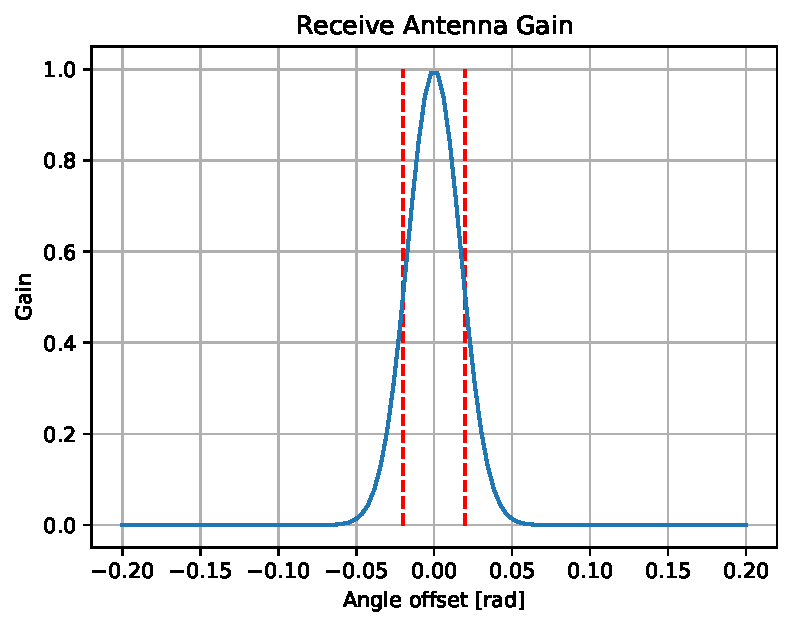
\includegraphics[width=0.68\textwidth]{figures/benchmark/rx_antenna_gain.pdf}
    \caption{Receive antenna gain in linear scale as a function of the beam offset. 
    The half-power offset angles are illustrated with red dashed lines.}
    \label{fig:beamwidth}
\end{figure}

\subsection{Numerical examples}\label{sec:ri_setup}


\bgroup
\def \arraystretch{1.25}
\begin{table}[tb]
    \centering
    \begin{tabular}{|l|c|c|c|}
    \hline
    \textbf{Name}              & \textbf{Symbol} & \textbf{Value}  & \textbf{Unit}\\ \hline
    Boresight SNR              & $SN_0$          & $50$ & -          \\ \hline
    Range resolution            & $d_\text{res}$  & $10$ & m  \\ \hline
    Monopulse antenna pattern slope  & $k_m$      & $1.6$ & -  \\ \hline
    Half of the $-3$dB beamwidth & $B$             & $0.02$ & rad         \\ \hline
    Probability of false alarm & $P_\text{fa}$   & $10^{-6}$ & -      \\ \hline
    Maximum number of dwells   & $n_\text{max}$  & $20$ & -  \\ \hline
    Dwell time                 & $\tau_d$          & $1e-3$ & s   \\ \hline
    Position                   & -               & $(0, 0)$ & m \\ \hline
    \end{tabular}
    \caption{Radar parameters in the simulations. Note that the probability of false alarm is only used to calculate the probability of detection.}
    \label{tab:radar_parameters}
\end{table}
\egroup

The RL approach for the RIS problem is evaluated in Monte Carlo simulations using numerical examples described in this section.
The simulation scenario contains the assumed monostatic radar presented in Section \ref{sec:system_description} at the position $x=0$ and $y=0$. 
The probability of detection is simulated based on the equation presented in \cite{vanKeuk1993}
\begin{equation}\label{eq:singer_1_pd}
    P_\text{d} = P_\text{fa}^{\frac{1}{1+SNR}},
\end{equation}
where $P_\text{fa}$ is the probability of false alarm.
However, $P_\text{fa}$ is only utilized to calculate the probability of detection, and false alarms are not included in the simulations.
The target is considered lost after $\nmax=20$ subsequent dwells without detection.

The angle offset of the radar beam is assumed to affect the SNR based on the following equation
\begin{equation} \label{eq:offset_snr}
    SNR = \sno~\exp{ - \ln{2}
        \frac
            {(\hat{\theta} - \theta)^2}
            {B^2}},
\end{equation}
where $\sno=50$ is the center beam SNR in a linear scale, $B=0.02$ is half of the -3dB beamwidth in radians, $\theta$ is target angle and $\hat{\theta} $ is the boresight angle. 
Furthermore, the parameters $\sno$ and $B$ are constant in the simulations. 
The radar beam is visualized in Figure \ref{fig:beamwidth}.
The fixed radar parameters are summarized in Table \ref{tab:radar_parameters}.

The monostatic radar is simulated in a tracking scenario using six trajectories introduced in Section \ref{sec:benchmark_trajectories}.
An IMM estimator is used to filter and predict the target states. 
The IMM estimator configuration is described in Section \ref{sec:cvca_imm}.
In Section \ref{sec:baseline_algorithm}, a baseline algorithm is presented to compare the RL approach to conventional RIS algorithm.
Lastly, different RL agent configurations are presented in Section \ref{sec:RL_config}.


\subsubsection{Benchmark trajectories} \label{sec:benchmark_trajectories}

\begin{figure}
    \centering
    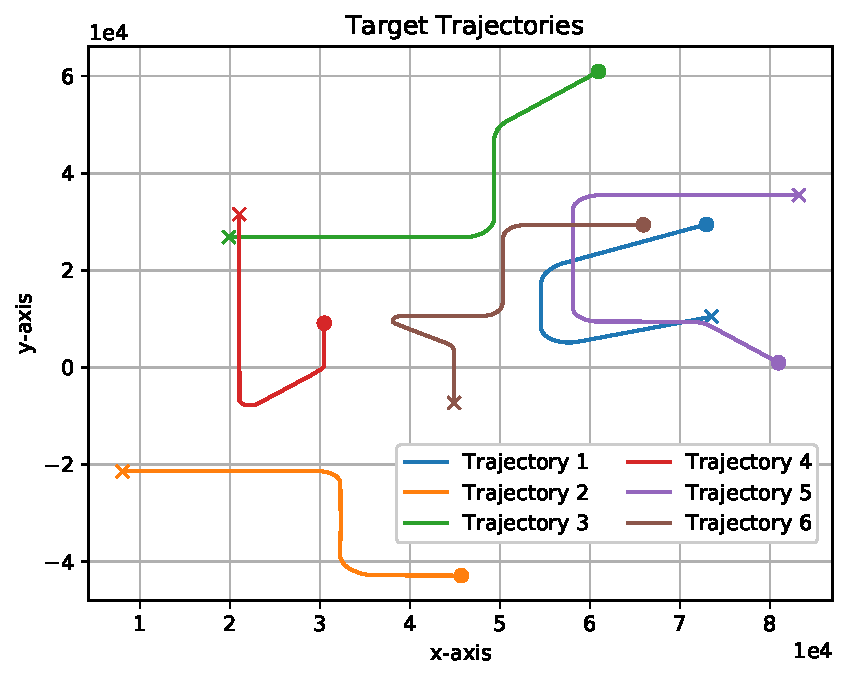
\includegraphics[width=0.8\textwidth]{figures/benchmark/trajectories.pdf}
    \caption{Six different target trajectories. The trajectories start from ``x'' and end to ``o''.}
    \label{fig:benchmark_trajectories}
\end{figure}

The target trajectories used in the simulations are based on a benchmark problem that was initially introduced in \cite{Blair1998}.
This original benchmark problem considered MTT in the presence of electronic countermeasures.
However, in the simulations here, the trajectories are used for the STT scenario and false alarms are neglected.
For the sake of simplicity, the spatial dimension is downsized from three-dimensional space to 2D space.
The 2D benchmark trajectories are shown in Figure \ref{fig:benchmark_trajectories}.

\begin{figure}
    \centering
    \begin{subfigure}{0.8\textwidth}
        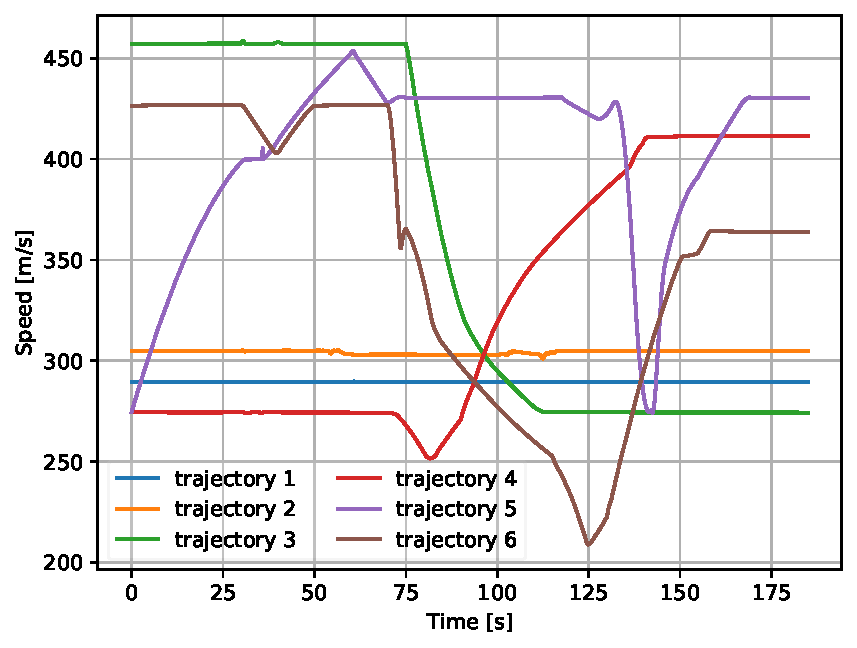
\includegraphics[width=\linewidth]{figures/benchmark/velocities.pdf}
        \caption{Speed of the target as a function of time.}
        \label{fig:benchmark_velocities}
    \end{subfigure}
    \hfill
    \begin{subfigure}{0.8\textwidth}
        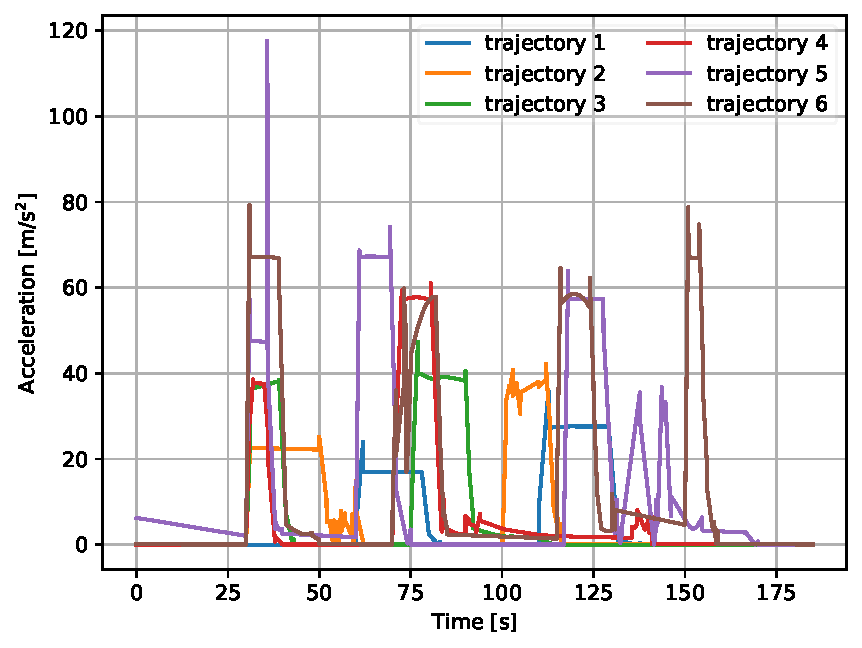
\includegraphics[width=\linewidth]{figures/benchmark/accelerations.pdf}
        \caption{Acceleration of the target as a function of time.}
        \label{fig:benchmark_acceleration}
    \end{subfigure}
    \label{fig:benchmark_vel_acc}
    \caption{Acceleration and velocity as a function of time for the benchmark trajectories. }
\end{figure}

The trajectories include different kinds of motion, such as constant-g turns, and straight motion with constant or non-constant velocity.
The target speed can range approximately from 210 m/s to 460 m/s, as can be seen in Figure \ref{fig:benchmark_velocities}.
The acceleration ranges approximately from 0 m/s$^2$ to 115 m/s$^2$ as seen in Figure \ref{fig:benchmark_acceleration}.
The benchmark trajectories are further summarized in Table \ref{tab:benchmark_table}, which contains the mean and the standard deviation values for acceleration and speed in each trajectory.
The values are utilized in Section \ref{sec:cvca_imm} to select the IMM estimator parameters. 


\begin{table}[htb]
    \centering
\begin{tabular}{|l|l|l|l|l|l|l|l|}
\hline
\multicolumn{2}{|l|}{}                                 & \textbf{T1} & \textbf{T2} & \textbf{T3} & \textbf{T4} & \textbf{T5} & \textbf{T6} \\ \hline
\multirow{2}{*}{\textbf{Velocity}}     & \textbf{mean} & 160.47      & 116.54      & 184.89      & 304.76      & 189.37      & 199.29      \\ \cline{2-8} 
                                       & \textbf{std}  & 78.92       & 139.4       & 198.54      & 90.8        & 181.85      & 170.52      \\ \hline
\multirow{2}{*}{\textbf{Acceleration}} & \textbf{mean} & 4.72        & 5.38        & 5.44        & 5.51        & 11.87       & 12.83       \\ \cline{2-8} 
                                       & \textbf{std}  & 9.23        & 10.87       & 12.65       & 13.79       & 20.06       & 22.06       \\ \hline
\end{tabular}
    \caption{Mean and standard deviation values of benchmark trajectories. Labels T1$\ldots$T6 denote trajectories from 1 to 6. The unit for velocity is m/s and m/s$^2$ for acceleration.}
    \label{tab:benchmark_table}
\end{table}


\subsubsection{CVCA-IMM estimator}\label{sec:cvca_imm}

The tracking filter employed in the simulations is an IMM estimator that uses two linear Kalman filters configured for two target motion models.
The motion models are the CV and the CA models, which were described in Section \ref{sec:target_models}.
In addition, the measurement model described in Section \ref{sec:measurement_model} is used in both filters.
This configuration is simple yet effective for the intended purpose.
The mode transition probability from CV to CA and CA to CV is set equal such that the state transition matrix is
\begin{equation}
    \vec{P} = 
\begin{bmatrix}
1 - \msp & \msp\\ 
\msp & 1 - \msp
\end{bmatrix},
\end{equation}
where $\msp$ is the mode transition probability.
This IMM estimator configuration will be called the CVCA-IMM estimator.

Such a configuration can be justified with three arguments.
First, the measurement and motion models are linear that is necessary for the linear Kalman filters introduced in Section \ref{sec:kalman_filter}.
However, it should be noted that the RL approach would apply even to non-linear filters without altering the RL formulation.
Secondly, only one mode probability is sufficient to present the mode probability based RL agent state since the IMM estimator has only two motion models.
Lastly, the CVCA-IMM estimator has only three parameters to be tuned.
These parameters are the acceleration noise variance for the CV model $\varcv$, the acceleration noise variance for the CA model $\varca$, and the mode transition probability $\msp$.

However, there is a problem that needs to be considered when using the two target models.
The dimension of the CV state vector \eqref{eq:x_mode1} and the CA state vector \eqref{eq:x_mode2} are different. 
Moreover, while the mode mixing equations \eqref{eq:imm_mx_init_x} and \eqref{eq:imm_mx_init_P} along with the state covariance fusion equations \eqref{eq:imm_fusion_x} and \eqref{eq:imm_fusion_P} require the dimensions to be equal.
In \cite{Granstroem2015}, an enhanced approach for mixing states with different dimensions was proposed.
However, here a simple approach is employed, which was also discussed in \cite{Granstroem2015}.
This approach augments the state estimate and corresponding error covariance matrix of the CV model with zeros.
According to \cite{Granstroem2015}, it corresponds to the situation in which the distributions of the accelerations in $x$ and $y$ coordinates are approximated with Dirac delta function.

The mode transition probabilities are defined for the processing time step $\dt=0.1$ because the tracker uses the time step to predict the future states recursively.
In other words, $\msp$ is the probability that the motion mode switches after time step $\dt$.
The time that is expected for the system to spend in a specific state is called sojourn time \cite{Simeonova2002}.
The transition probability $\msp$ can be then calculated by the following equation
\begin{equation}
   \msp = \frac{\dt}{T_s},
\end{equation}
where $T_s$ is the sojourn time.
However, the sojourn time is typically tedious to estimate for a target, especially when using non-optimal motion models \cite{Simeonova2002}.
As described in \cite{Simeonova2002}, higher transition probabilities lead to lower peak square errors in the predicted states, but the mean square error can be higher.
The parameters $\msp=0.028$, $\varcv=747.5$ and $\varca=74.7$ were found empirically by simulating the CVCA-IMM estimator with different parameter combinations.
The selected $\msp$ corresponds to approximately $3.6s$ sojourn time.

\begin{figure}[bt]
    \centering
    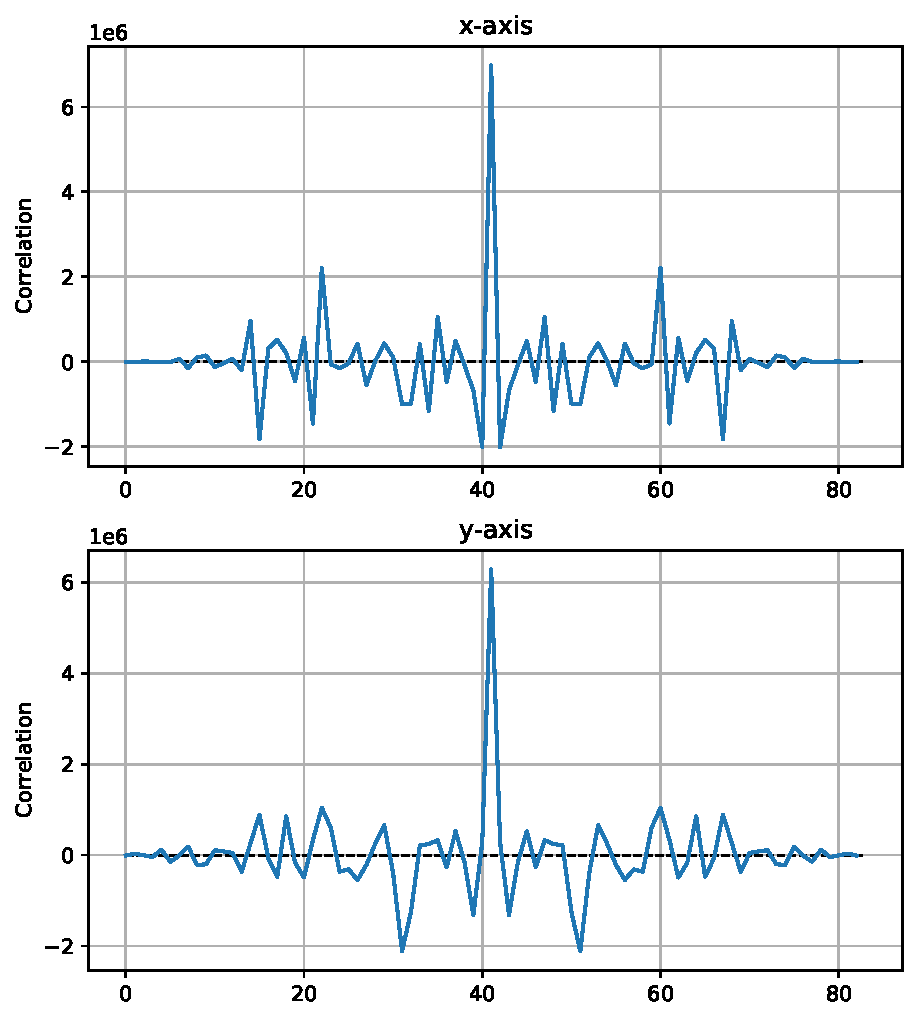
\includegraphics[width=0.8\linewidth]{figures/benchmark/IMM/correlation_imm.pdf}
    \caption{Auto-correlation of the innovation sequence when the CVCA-IMM estimator is applied for trajectory six.}
    \label{fig:auto_correlation}
\end{figure}

The performance of the tracking filter can be examined by visualizing the auto-correlation function of the innovation sequence.
In the ideal case, the auto-correlation function should not exhibit a significant correlation, which would indicate that the innovation sequence is approximately non-correlated noise.
Figure \ref{fig:auto_correlation} shows the auto-correlation function of the innovation sequence in $x$ and $y$ axis evaluated on trajectory 6, which is the trajectory with the sharpest maneuvers.
Figure \ref{fig:auto_correlation} shows that the auto-correlation function is mainly random, indicating that the innovation sequence does not have a significant temporal correlation.
Thus, the CVCA-IMM estimator functions in the tracking scenario as desired.



\subsubsection{Baseline algorithm} \label{sec:baseline_algorithm}

A baseline algorithm is utilized to compare the RL approach against an existing RIS algorithm.
The baseline algorithm for controlling the RI is based on an approach proposed in \cite{Daeipour1994}.
This algorithm is error covariance matrix based algorithm that is used to optimize
\begin{equation}\label{eq:baseline_ineq}
    \begin{array}{ll}
         & \max_{t_r} t_r \\
        \text{s.t.} & \sigma_\theta(t+\ri|t) \leq V_0 B, 
    \end{array}
\end{equation}
where $V_0$ is the track sharpness parameter, and $\sigma_\theta(t+\ri|t)$ is the standard deviation of the error of the predicted azimuth angle.
The longest RI to satisfy the constraint is found by propagating the predictive equations of the CVCA-IMM estimator with the time step $\dt$.
The track sharpness $V_0$ affects the risk of losing the tracks and needs to be tuned for the specific IMM estimator.
The performance with different values of $V_0$ is discussed in Section \ref{sec:against_baseline}.

\subsubsection{Reinforcement learning agent configuration}\label{sec:RL_config}

Various RL agents are configured such that it is possible to identify effective state spaces from the states discussed in Section \ref{sec:states}, and to determine if using a myopic policy is sufficient.
All the agents use the Q-learning algorithm with \egreedy exploration.

The learning rate $\alpha$ is controlled adaptively by using the asynchronous update strategy \cite{Even-Dar2003}.
Thus, the learning rate is defined as a function of time as follows
\begin{equation}
    \alpha_k = \frac{1}{\#(s, a, k)^\omega},
\end{equation}
where $\#(s, a, k)$ is the number of times action $a$ is taken from state $s$ at time instance $k$, and $\omega \in (0.5, 1)$ controls how fast $\alpha_k$ decays.
For myopic agents with $\lambda=0$, the parameter $\omega=1$ is used such that the empirical means of the rewards are calculated.
For non-myopic agents, the corresponding values are set to $\lambda=0.7$ and $\omega=0.75$. 

The direct selection action space $\Asdir$ is used with $N_a=10,$ $\tmin=0.1s$ and $\tmax=7.5s$.
State variables used for the agents are the most recent innovation, the probability of the CV mode, and the previous RI.
The discretization parameter was set to $N_d=10$, such that $N_s=12$ for the state spaces that does not use the previous RI, and $N_s=102$ otherwise.
The configurations of the agents are shown in Table \ref{tab:agent_configurations}. The ID's from the table are used in results presented in Section \ref{sec:ri_sim}.

\begin{table}[t]
    \centering
    \begin{tabular}{|c | c | c |c |}
        \hline
        \textbf{Agent ID} & \textbf{State}  & $\lambda$  &  $\omega$ \\
        \hline
        0 & innovation & 0.0 & 1.0 \\ \hline
        1 & innovation & 0.7 & 0.75 \\ \hline
        2 & innovation \& previous RI &  0.0 & 1.0 \\ \hline
        3 & innovation \& previous RI & 0.7 & 0.75 \\ \hline
        4 & mode probability &  0.0 & 1.0 \\ \hline
        5 & mode probability & 0.7 & 0.75 \\ \hline 
        6 & mode probability \& previous RI &  0.0 & 1.0 \\ \hline 
        7 & mode probability \& previous RI & 0.7 & 0.75 \\
        \hline
    \end{tabular}
    \caption{Agent configurations.}
    \label{tab:agent_configurations}
\end{table}


\subsection{Simulation results}\label{sec:ri_sim}

The performance is evaluated by measures based on the tracking load in equation \eqref{eq:load} and the probability of losing tracks. 
Mean tracking load refers to the following measure
\begin{equation} 
    L_\text{mean} = \mathbb{E}_{i \sim P_T(i)} \left[ L_\text{AM}(i) | \pi \right],
\end{equation}
where $L_\text{AM}(i)$ is the arithmetic mean of temporal tracking load values in trajectory $i$,  $\pi$ is the RIS policy, and the trajectories are sampled from the distribution $P_T(i)$.
Therefore, the mean tracking load is evaluated in Monte Carlo simulations as follows
\begin{equation}\label{eq:criterion_load}
    L_\text{mean} \approx \frac{1}{\Ne} \sum_{n=0}^{\Ne-1} \frac{1}{K_m}\sum_{k=0}^{K_m-1} L_{mk},
\end{equation}
where $\Ne$ is number of episodes, $K_m$ is number of steps in episode $m$, and $L_{mk}$ is the temporal tracking load in episode $m$ at step $k$.
An episode refers to simulating a sampled trajectory until the end of the trajectory or when the target is lost.

The ability to track targets without losing them is measured in terms of Probability to Lose a Track (PLT).
The PLT refers to the probability $\Pr{\text{Track lost}|\pi, i}$ that is the probability to lose a target in a certain trajectory $i$ given a RIS policy $\pi$.
On the other hand, mean PLT is used to refer to the probability
\begin{equation}
    P_\text{mean} = \Pr{\text{Track lost}|\pi, P_T(i)}
\end{equation} that is similar to the PLT but the trajectories are sampled from the distribution $P_T(i)$.
Therefore, the mean PLT is evaluated in Monte Carlo simulations as follows
\begin{equation}\label{eq:criterion_lost}
\   P_\text{mean} \approx \frac{1}{\Ne} \sum_{m=0}^{\Ne-1} \vec{1}_{\text{TrackLost}(m)},
\end{equation}
where $\vec{1}_{\text{TrackLost}(m)}$ is one if the track is lost in episode $m$ and zero otherwise.

The RL approach for RIS was evaluated in the simulation setup described in Section \ref{sec:ri_setup}.
The objectives of the simulations were to
\begin{itemize}
    \item identify effective state space,
    \item determine if using a myopic policy is sufficient,
    \item evaluate the mean PLT and the mean tracking load during the learning,
    \item evaluate the amount of learning required to achieve a certain level of performance,
    \item determine the connection between $\closs$ and the PLT, and
    \item compare the RL approach against the baseline algorithm.
\end{itemize}
The first four of these will be covered in Section \ref{sec:training}, and the last two will be covered in Section \ref{sec:against_baseline}.

\subsubsection{Reinforcement learning agent training}\label{sec:training}

RL agents with various configurations were trained by uniformly sampling the target trajectories from the six benchmark trajectories.
Each agent was trained for $4000$ episodes, which corresponds to training an agent on each trajectory approximately for $667$ times on average.
The exploration probability is initially $\epsilon=0.2$ and between each episode, the epsilon decays by a factor of $0.99867$, which results in $\epsilon=0.001$ on the last training episode.
The cost of losing a track $\closs$ was set to $0.2$.

Target policies and behavior policies, discussed in Section \ref{sec:q_learning}, were evaluated with various numbers of training episodes.
In the Q-learning algorithm, the target policy chooses the action with the highest Q-value unlike the behavior policy, which also takes random actions with probability $\epsilon$.
The amount of learning needed to achieve a certain level of performance was evaluated by examining the performance of a target policy.
It corresponds to the situation where learning ends after a certain number of episodes, and after that, the agent uses only the target policy.
On the other hand, performance while learning was evaluated by examining the performance of a behavior policy.
The performance of a target policy will be called target performance, and similarly, the performance of a behavior policy is called behavior performance.

\begin{figure}
    \centering
    \begin{subfigure}[b]{0.8\textwidth}
        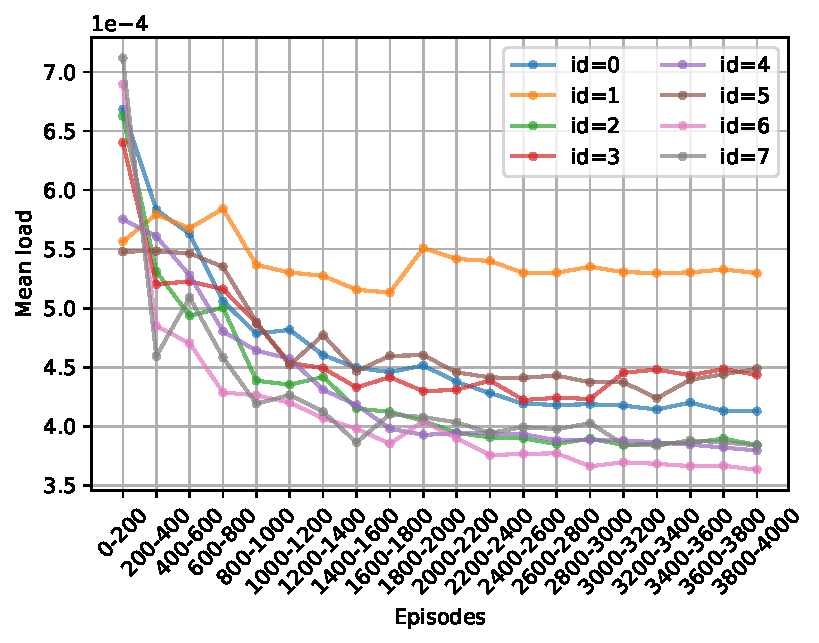
\includegraphics[width=\textwidth]{figures/benchmark/Training/online_load.pdf}
        \caption{Mean tracking load.}
        \label{fig:online_load}
    \end{subfigure}
    \hfill
    \begin{subfigure}[b]{0.8\textwidth}
        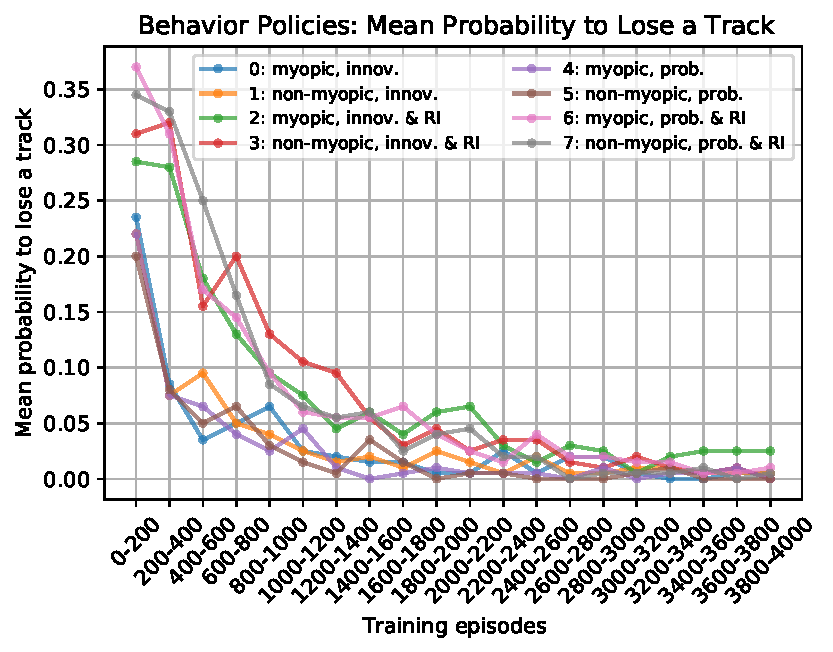
\includegraphics[width=\textwidth]{figures/benchmark/Training/online_plt.pdf}
        \caption{Mean probability to lose a track.}
        \label{fig:online_lost}
    \end{subfigure}
    \caption{Performance of behavior policies.}
    \label{fig:online_performance}
\end{figure}

\begin{figure}
    \centering
    \begin{subfigure}[b]{0.8\textwidth}
        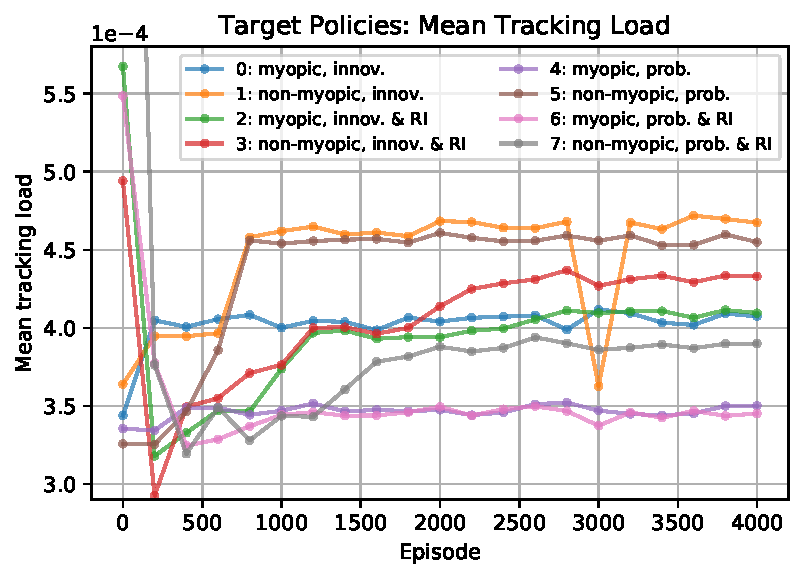
\includegraphics[width=\textwidth]{figures/benchmark/Training/offline_load.pdf}
        \caption{Mean tracking load.}
        \label{fig:offline_load}
    \end{subfigure}
    \hfill
    \begin{subfigure}[b]{0.8\textwidth}
        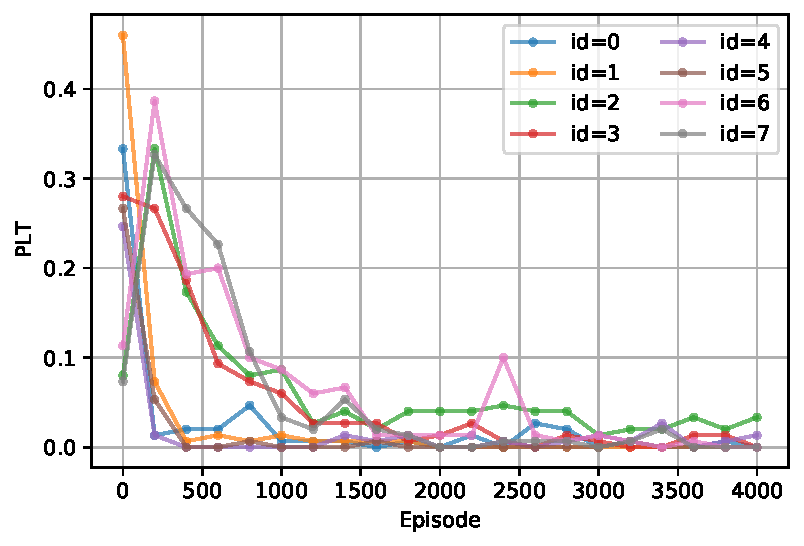
\includegraphics[width=\textwidth]{figures/benchmark/Training/offline_plt.pdf}
        \caption{Probability to lose a track in an episode.}
        \label{fig:offline_lost}
    \end{subfigure}
    \caption{
        Offline performance estimated from Monte Carlo simulations.
    }
    \label{fig:offline_performance}
\end{figure}

The behavior policies were evaluated every 200 episodes using the data from the past $\Ne=200$ training episodes to calculate \eqref{eq:criterion_load} and \eqref{eq:criterion_lost}.
The behavior performance is shown in Figure \ref{fig:online_performance}.
On the other hand, snapshots of the target policies were saved every 200 episodes while training, and those policies were evaluated using Monte Carlo simulations.
Each snapshot of a policy was evaluated with 25 Monte Carlo iterations per trajectory.
Thus the equations \eqref{eq:criterion_load} and \eqref{eq:criterion_lost} were evaluated using $\Ne=150$ episodes.
The target performance is shown in Figure \ref{fig:offline_performance}.


Figure \ref{fig:online_performance} shows that the behavior performance is slowly improving between the episodes with a particular trend.
On the other hand, the trend in the target performance is not as apparent, as shown in Figure \ref{fig:offline_performance}.
Notably, the mean tracking load in Figure \ref{fig:offline_load} meets its lower limit quite fast, but the mean PLT in Figure \ref{fig:offline_lost} requires more time to converge to tolerable levels.
Differences in the target and the behavior policies may explain the differences between the target performance and the behavior performance.
The behavior policy takes random actions that increase the tracking load compared to the target policy, which is purely exploiting.
For the agent, it is undoubtedly more challenging to learn the PLT than the tracking load.
Therefore, the target policies had fast improvement in the tracking load, as shown in Figure \ref{fig:offline_load}. 
The mean tracking load even rises slightly when the agent has learned more because the agent becomes more conscious about losing tracks with longer RIs.
Meanwhile, the PLT takes more training episodes to converge to low values, as shown in Figure \ref{fig:offline_lost}.
Thus, learning to not lose tracks will take more training episodes.


In episodes approximately up to 1500, two distinct clusters can be seen in Figures \ref{fig:online_lost} and \ref{fig:offline_lost}.
The clusters divide the agents between using the 1D state spaces and the 2D state spaces.
The terminology 1D and 2D refer to the state spaces without and with the augmented most recent RI, respectively.
The clusters are caused by the fact that the 2D state spaces have higher cardinality than the 1D state spaces, thus requiring more state-action pairs to be explored.
Therefore, the agents with 1D state space learn faster than agents with 2D state space.
At the end of the training, the agents with 2D spaces have slightly lower tracking load with similar PLT.
Therefore, the higher dimensional state space seems to improve the performance marginally if the learning speed is not a subject of concern.

\begin{table}[tb]
    \centering
    \begin{tabular}{|l|l|l|l|l|l|l|}
        \hline
        \textbf{Agent} & \textbf{T1} & \textbf{T2} & \textbf{T3} & \textbf{T4} & \textbf{T5} & \textbf{T6} \\ \hline
        0: myopic, innov. & 0 & 0 & 0 & 0.03  & 0     & 0     \\ \hline
        1: non-myopic, innov. & 0 & 0 & 0 & 0.005 & 0     & 0     \\ \hline
        2: myopic, innov. \& RI & 0 & 0 & 0 & 0.14  & 0     & 0.03  \\ \hline
        3: non-myopic, innov. \& RI & 0 & 0 & 0 & 0.005 & 0     & 0.01  \\ \hline
        4: myopic, prob. & 0 & 0 & 0 & 0.04  & 0.005 & 0.005 \\ \hline
        5: non-myopic, prob. & 0 & 0 & 0 & 0     & 0     & 0     \\ \hline
        6: myopic, prob. \& RI & 0 & 0 & 0 & 0.07  & 0     & 0     \\ \hline
        7: non-myopic, prob. \& RI & 0 & 0 & 0 & 0.035 & 0     & 0.005 \\ \hline
    \end{tabular}
    \caption{Mean Probability to Lose a Track (PLT) for target policies after 4000 episodes of learning. T1 $\ldots$ T6 denote target trajectories from 1 to 6.}
    \label{tab:plt_comparison}
\end{table}

Another distinct performance differences between the configurations can be seen for myopic and non-myopic agents.
With no exception, the non-myopic agents have a higher tracking load than the corresponding myopic agent with the same state space. 
For example, the agent with $\text{ID}=1$ is non-myopic variant of the myopic agent with $\text{ID}=0$.
The difference could be originated from two reasons.
First, the non-myopic agents are more conscious about losing tracks because the long-term consequences for actions are considered.
Especially from Table \ref{tab:plt_comparison}, it can be seen that after learning for 4000 episodes, the mean PLT of target policies is multiple times higher for myopic agents than for non-myopic agents.
The second reason may be that for the non-myopic policies, the Q-values converge slower than for the myopic policies.
Thus, training a non-myopic agent to its full potential generally requires more training episodes than needed for a myopic agent.


\subsubsection{Performance against the baseline algorithm} \label{sec:against_baseline}


In terms of fast learning speed, low mean PLT, and low mean tracking load, the agent with $\text{ID}=4$ was identified to have desirable performance.
The agent uses the mode probabilities as states and is based on a myopic policy.

\begin{figure}
    \centering
    \begin{subfigure}[b]{0.45\textwidth}
        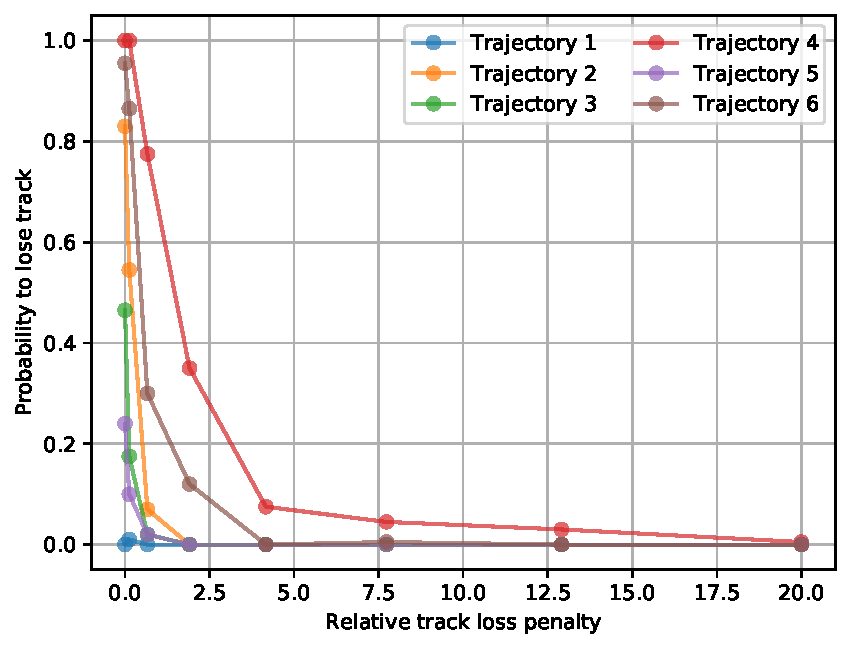
\includegraphics[width=\linewidth]{figures/benchmark/Simulations/plt_agent.pdf}
        \caption{The PLT of the RL agent.}
        \label{fig:penalty_plt}
    \end{subfigure}
    \hfill
    \begin{subfigure}[b]{0.45\textwidth}
        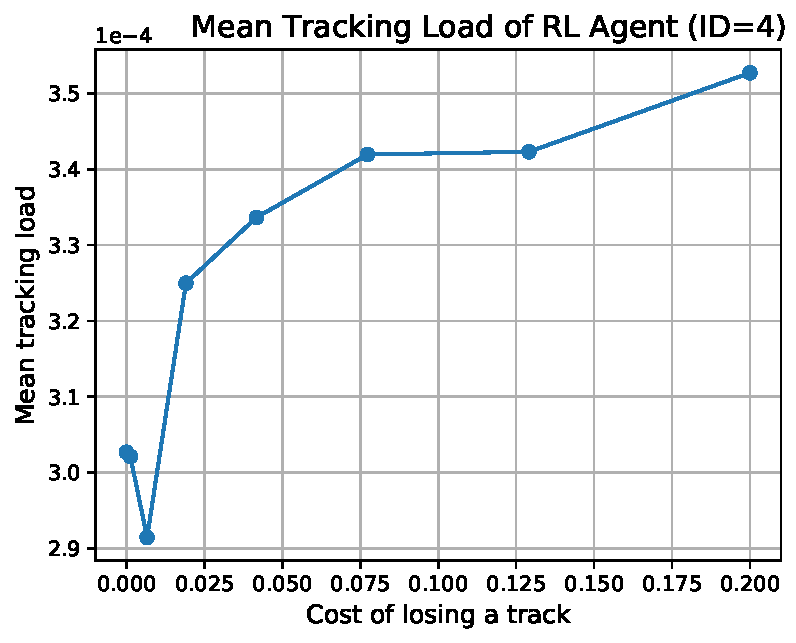
\includegraphics[width=\linewidth]{figures/benchmark/Simulations/tracking_load_agent.pdf}
        \caption{The mean tracking load of the RL agent.}
        \label{fig:penalty_load}
    \end{subfigure}
    \begin{subfigure}[b]{0.45\textwidth}
        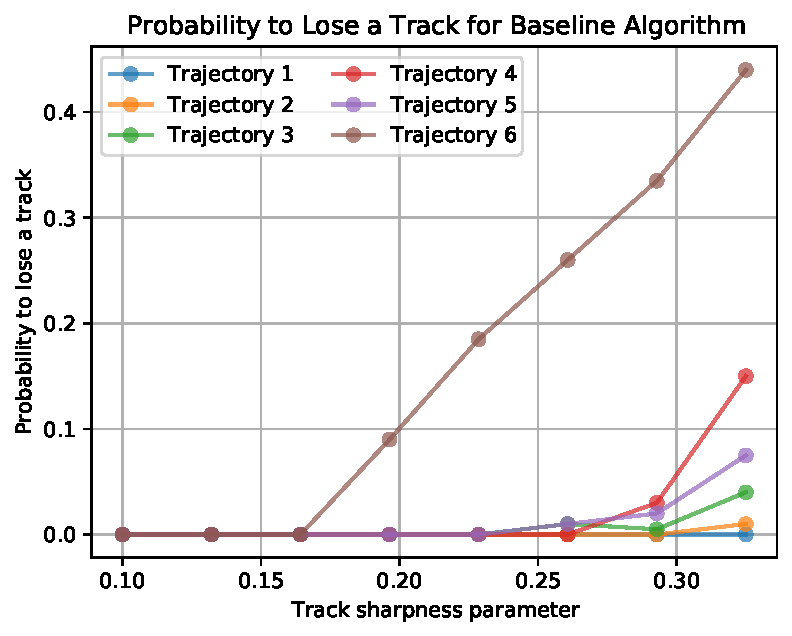
\includegraphics[width=\linewidth]{figures/benchmark/Simulations/plt_baseline.pdf}
        \caption{The PLT of the baseline algorithm.}
        \label{fig:baseline_plt}
    \end{subfigure}
    \hfill
    \begin{subfigure}[b]{0.45\textwidth}
        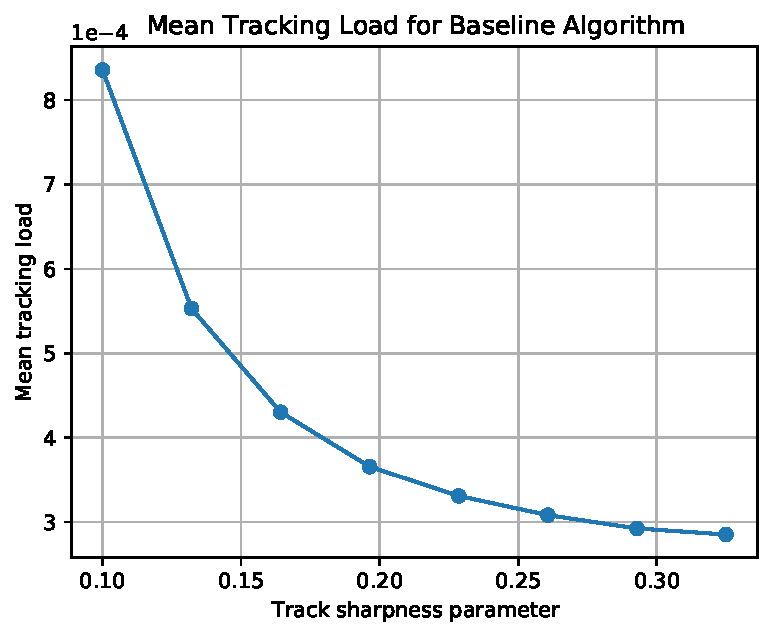
\includegraphics[width=\linewidth]{figures/benchmark/Simulations/tracking_load_baseline.pdf}
        \caption{The mean tracking load of the baseline algorithm.}
        \label{fig:baseline_load}
    \end{subfigure}
    \caption{The reinforcement learning (RL) agent with ID=4 and the baseline algorithms compared with different parameterizations in terms of Probability to Lose a Track (PLT) and mean tracking load.}
    \label{fig:comparison}
\end{figure}

The RL agent was trained and evaluated with various values of $\closs$.
The figures \ref{fig:penalty_plt} and \ref{fig:penalty_load} shows the PLT and the mean tracking load, respectively.
It can be seen that the low cost of losing a track results in low mean tracking load but high PLT.
Additionally, the high cost of losing a track results in high mean tracking load but low PLT.
The baseline algorithm was also evaluated with different track sharpness values.
Figure \ref{fig:baseline_plt} shows how the track sharpness parameter $V_0$ affects the PLT.
In addition, Figure \ref{fig:baseline_load} shows the mean tracking load with different track sharpness parameters.
Each value of $\closs$ and $V_0$ were evaluated using $200$ Monte Carlo iterations per trajectory.
Figure \ref{fig:comparison} can be used to compare the RL approach and the baseline algorithm.
For the baseline algorithm, the trajectory 6 is the most difficult to maintain while the trajectory 4 is the most difficult for the RL algorithm.

Using figures \ref{fig:penalty_plt} and \ref{fig:baseline_plt}, the parameters of the RL agent and the baseline algorithm were tuned to achieve an approximately equal PLT to evaluate the tracking load in equation \eqref{eq:load}, the selected RIs, and euclidean distances between the target positions and the predicted target positions.
Thus, the parameters $\closs = 0.2$ and $V_0=0.164$ were selected.
With the corresponding parameters, the RL agent lost the target in trajectory 4 one time out of 200 Monte Carlo iterations.
The baseline algorithm did not lose any tracks in the Monte Carlo simulations.
The cost of losing a track $\closs=0.2$ is equal to the value used in Section \ref{sec:training}.
However, the policy of the agent with the identical configuration in Section \ref{sec:training} is different from the policy evaluated here because the agent was trained again.
The policy evaluated here is shown in Figure \ref{fig:policy_id4}.

\begin{figure}[tb]
    \centering
    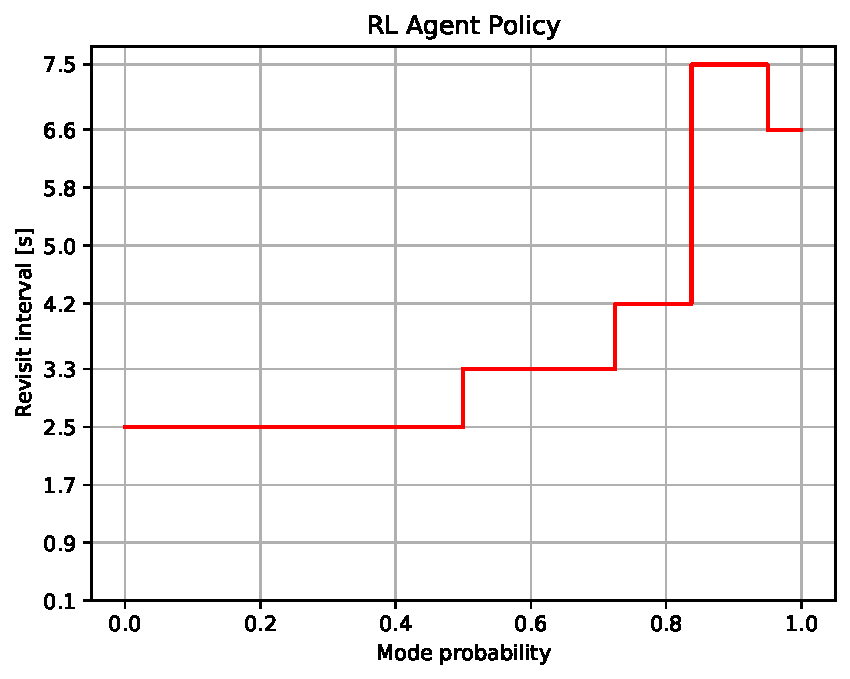
\includegraphics[width=.8\linewidth]{figures/benchmark/Training/policy.pdf}
    \caption{Policy of the RL agent with ID=4. The state on x-axis is the probability of the CV mode, and the agent chooses the revisit interval on y-axis when in a corresponding state.}
    \label{fig:policy_id4}
\end{figure}

The tracking load is shown for each trajectory in Figure \ref{fig:tracking_load_comparison}.
For trajectories 1, 5, and 6, the tracking load for the baseline algorithm and the RL agent are approximately equal when the target is not maneuvering.
On the other hand, the RL agent can keep the load smaller when the target turns and the tracking load peaks are induced.
In trajectories 2 and 3, the target approaches the radar. 
Therefore, the baseline algorithm decreases the RI gradually, which increases the tracking load.
Based on the experience, the RL agent is confident enough that the corresponding situation does not require smaller RI such that a lower tracking load is achieved.
In trajectory 4, the difference between the baseline algorithm and the RL algorithm is the most apparent.
As with trajectories 2 and 3, the lower tracking load can be related to the range of the target.
The RL agent is more eager to take the risk of using longer RIs because the experience does indicate that using such RIs does not have a high risk of losing track.
However, the PLT is at $0.5\%$, which is higher compared to the other tracks because the state space may not generalize the corresponding trajectory well enough.
It could be possible that the track is lost with a lower probability if the target range would be included to the state presentation.

\begin{figure}
    \centering
    \begin{subfigure}[b]{0.45\textwidth}
        \centering
        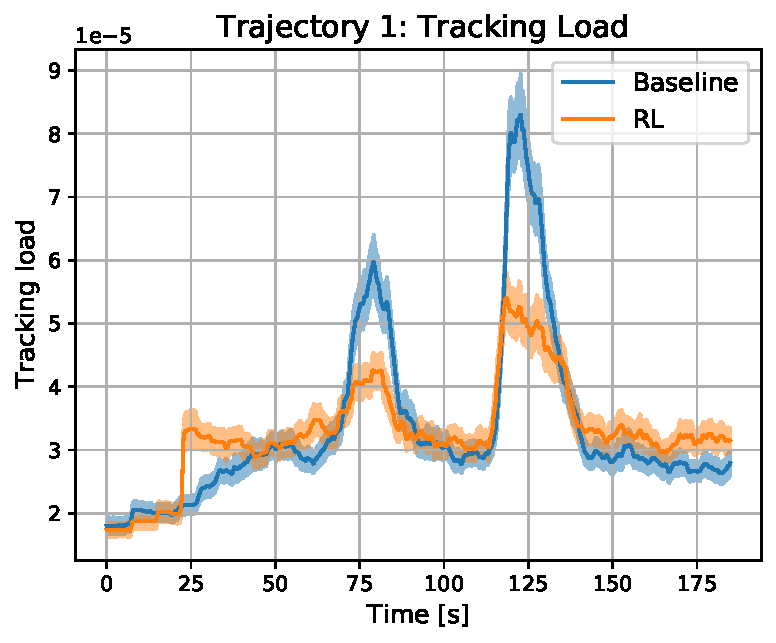
\includegraphics[width=\linewidth]{figures/benchmark/Simulations/tracking_load_0.pdf}
        \caption{Trajectory 1.}
        \label{fig:TL_T1}
    \end{subfigure}
    \hfill
    \begin{subfigure}[b]{0.45\textwidth}
        \centering
        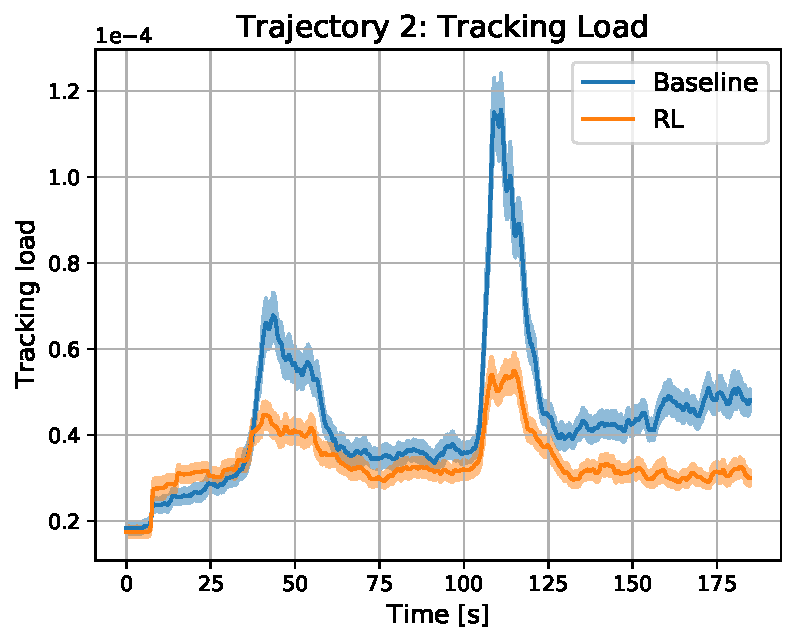
\includegraphics[width=\linewidth]{figures/benchmark/Simulations/tracking_load_1.pdf}
        \caption{Trajectory 2.}
        \label{fig:TL_T2}
    \end{subfigure}
    \hfill
    \begin{subfigure}[b]{0.45\textwidth}
        \centering
        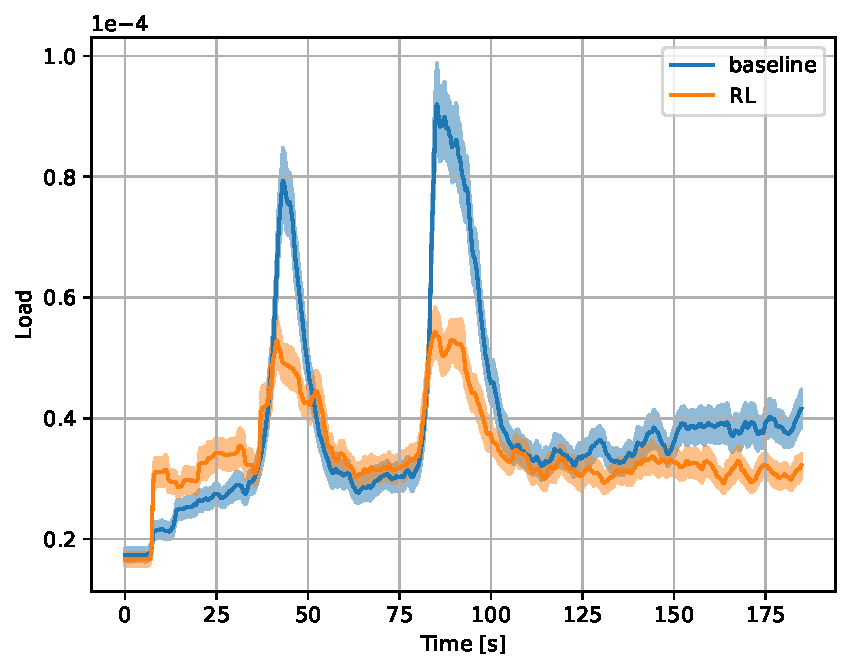
\includegraphics[width=\linewidth]{figures/benchmark/Simulations/tracking_load_2.pdf}
        \caption{Trajectory 3.}
        \label{fig:TL_T3}
    \end{subfigure}
    \hfill
    \begin{subfigure}[b]{0.45\textwidth}
        \centering
        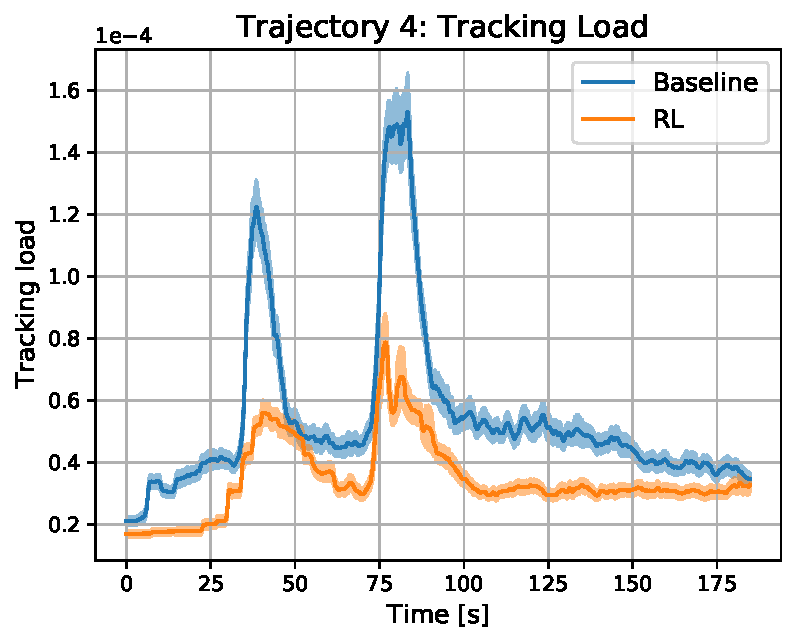
\includegraphics[width=\linewidth]{figures/benchmark/Simulations/tracking_load_3.pdf}
        \caption{Trajectory 4.}
        \label{fig:TL_T4}
    \end{subfigure}
    \hfill
    \begin{subfigure}[b]{0.45\textwidth}
        \centering
        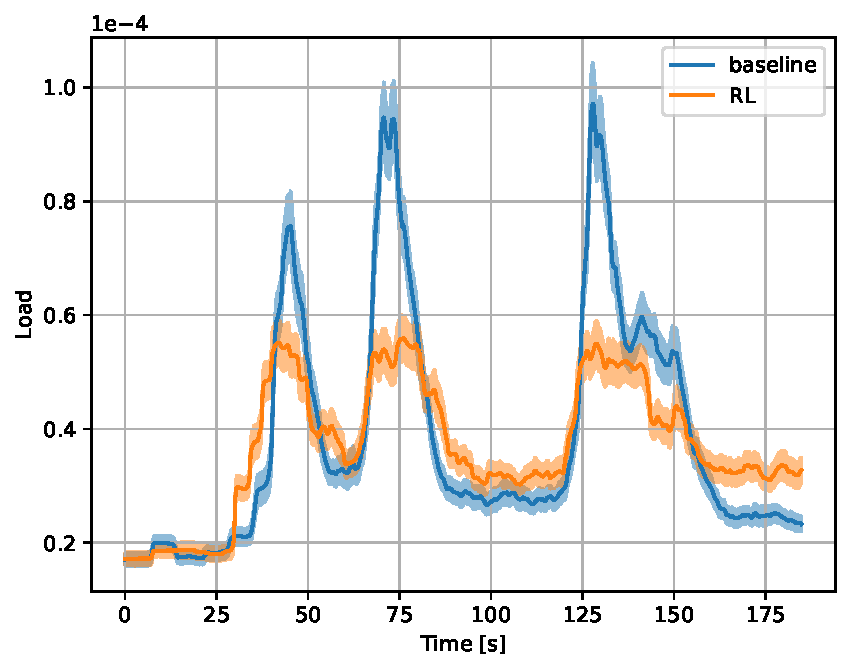
\includegraphics[width=\linewidth]{figures/benchmark/Simulations/tracking_load_4.pdf}
        \caption{Trajectory 5.}
        \label{fig:TL_T5}
    \end{subfigure}
    \hfill
    \begin{subfigure}[b]{0.45\textwidth}
        \centering
        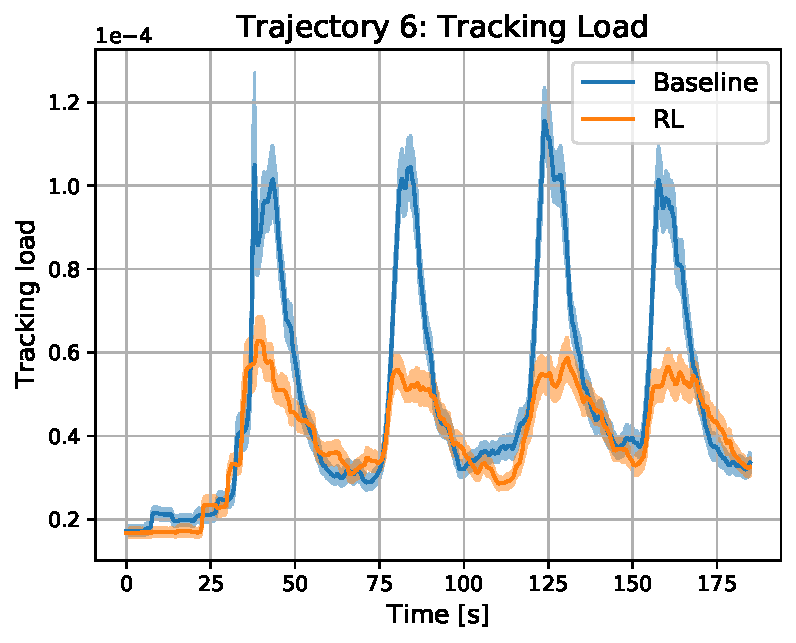
\includegraphics[width=\linewidth]{figures/benchmark/Simulations/tracking_load_5.pdf}
        \caption{Trajectory 6.}
        \label{fig:TL_T6}
    \end{subfigure}
    \caption{Comparing the proposed reinforcement learning approach to the baseline algorithm in terms of tracking load.
    The figures provide expected tracking load with 95\% confidence intervals.}
    \label{fig:tracking_load_comparison}
\end{figure}


In Figure \ref{fig:revisit_interval_comparison}, the selected RIs are shown for each benchmark trajectory.
The connection between the selected RIs and the tracking load is apparent.
When lower RIs are used, also higher tracking load can be seen in Figure \ref{fig:tracking_load_comparison}, and vice versa.
The significant difference between the baseline algorithm and the RL agent is that the baseline algorithm often used shorter RIs when the target maneuvers sharply and therefore the tracking load was increased.

\begin{figure}
    \centering
    \begin{subfigure}[b]{0.45\textwidth}
        \centering
        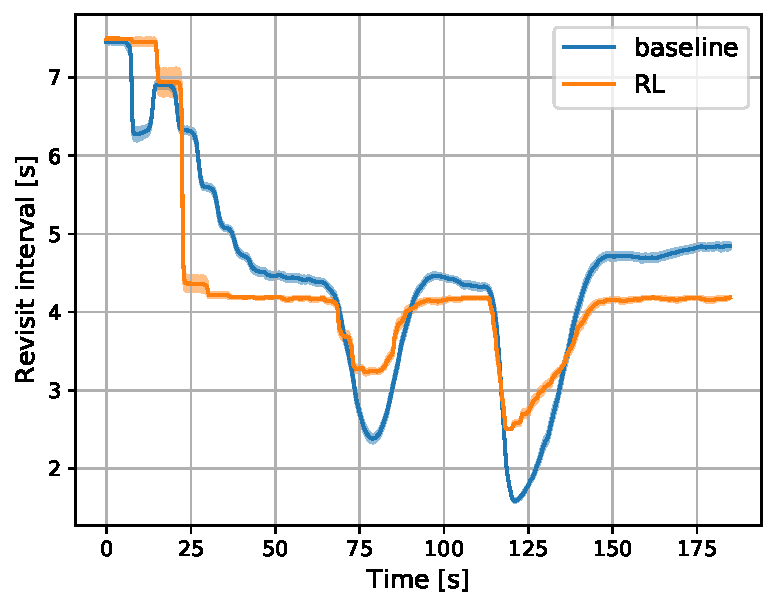
\includegraphics[width=\linewidth]{figures/benchmark/Simulations/revisit_intervals_0.pdf}
        \caption{Trajectory 1.}
        \label{fig:RI_T1}
    \end{subfigure}
    \hfill
    \begin{subfigure}[b]{0.45\textwidth}
        \centering
        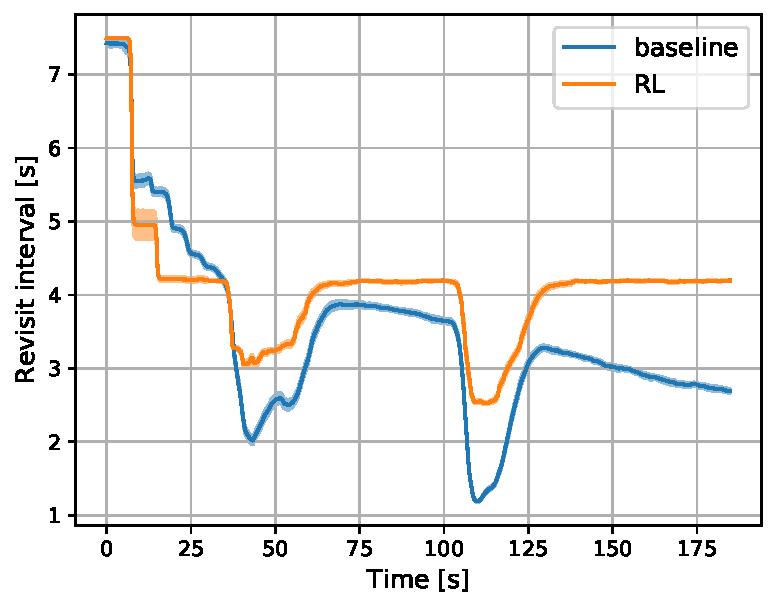
\includegraphics[width=\linewidth]{figures/benchmark/Simulations/revisit_intervals_1.pdf}
        \caption{Trajectory 2.}
        \label{fig:RI_T2}
    \end{subfigure}
    \hfill
    \begin{subfigure}[b]{0.45\textwidth}
        \centering
        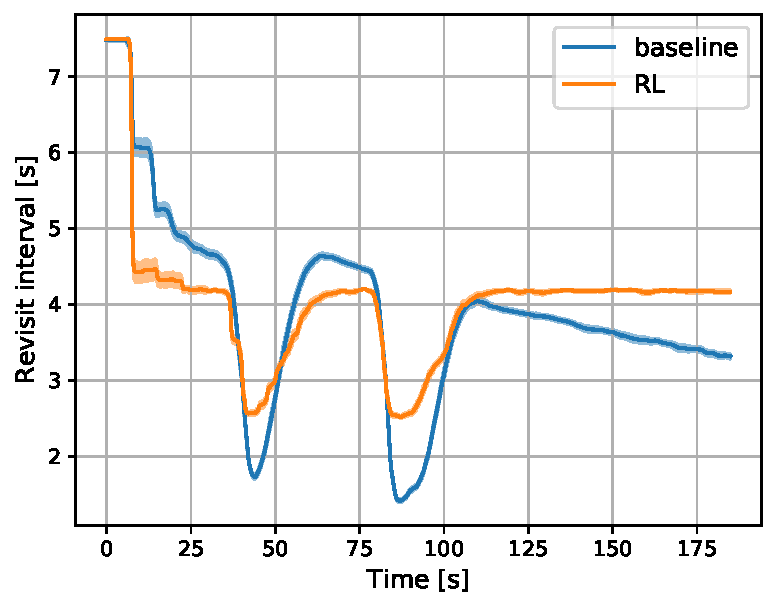
\includegraphics[width=\linewidth]{figures/benchmark/Simulations/revisit_intervals_2.pdf}
        \caption{Trajectory 3.}
        \label{fig:RI_T3}
    \end{subfigure}
    \hfill
    \begin{subfigure}[b]{0.45\textwidth}
        \centering
        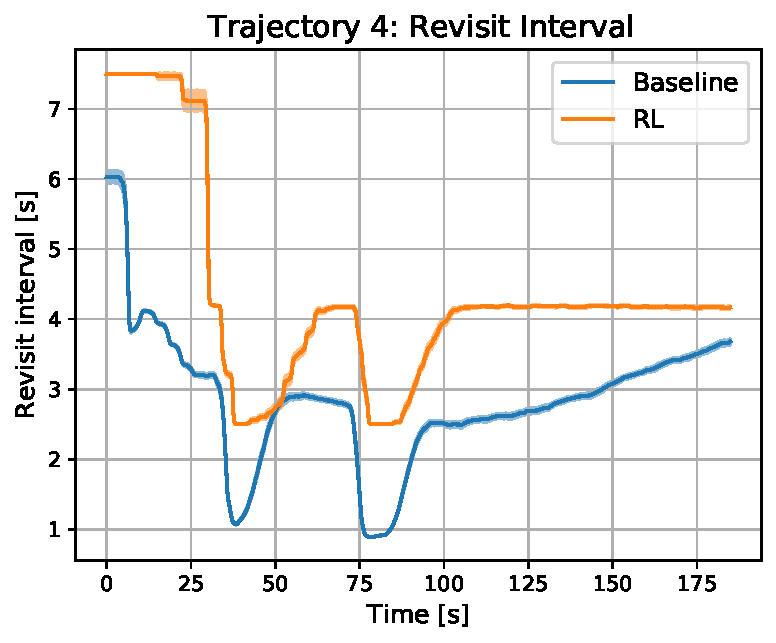
\includegraphics[width=\linewidth]{figures/benchmark/Simulations/revisit_intervals_3.pdf}
        \caption{Trajectory 4.}
        \label{fig:RI_T4}
    \end{subfigure}
    \hfill
    \begin{subfigure}[b]{0.45\textwidth}
        \centering
        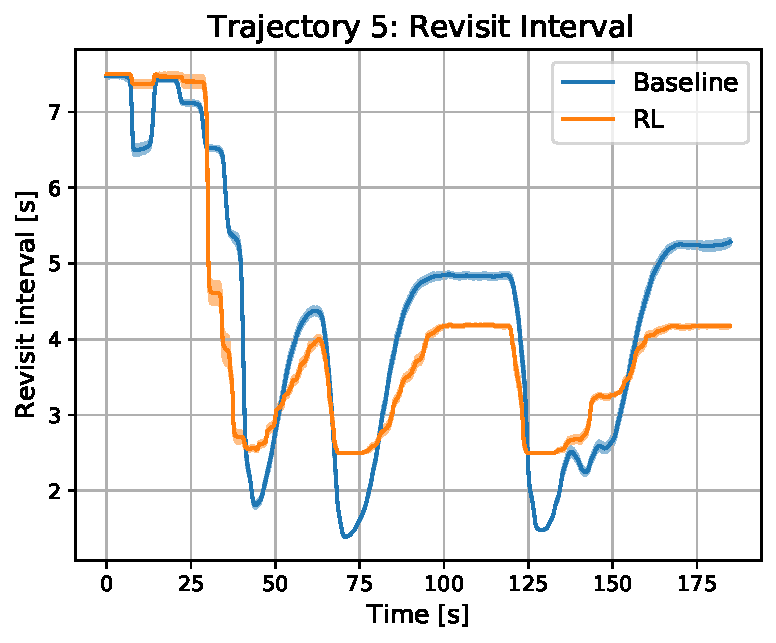
\includegraphics[width=\linewidth]{figures/benchmark/Simulations/revisit_intervals_4.pdf}
        \caption{Trajectory 5.}
        \label{fig:RI_T5}
    \end{subfigure}
    \hfill
    \begin{subfigure}[b]{0.45\textwidth}
        \centering
        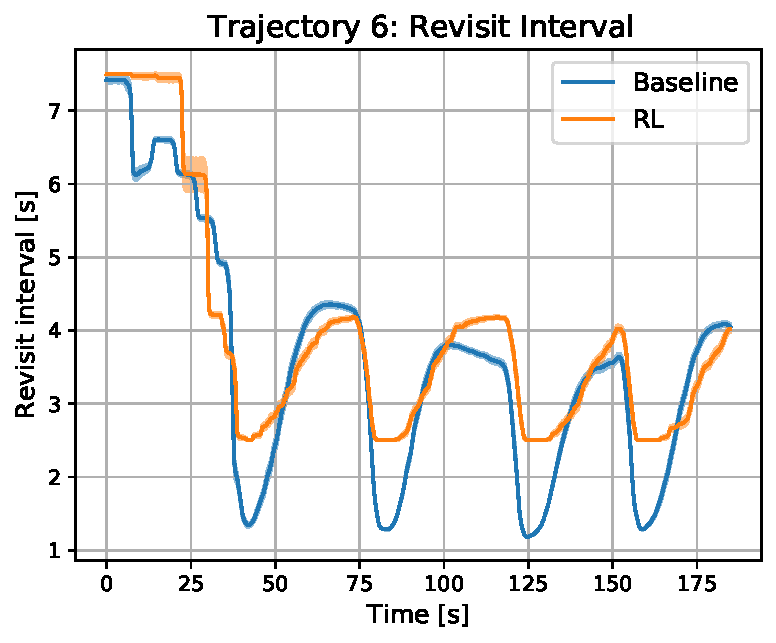
\includegraphics[width=\linewidth]{figures/benchmark/Simulations/revisit_intervals_5.pdf}
        \caption{Trajectory 6.}
        \label{fig:RI_T6}
    \end{subfigure}
    \caption{Comparing the proposed reinforcement learning approach to the baseline algorithm in terms of revisit intervals.
    The figures provide expected revisit interval with 95\% confidence intervals.}
    \label{fig:revisit_interval_comparison}
\end{figure}

Figure \ref{fig:position_error_comparison} shows the errors in the predictive target position estimates.
The errors for the baseline and the RL algorithms are mostly similar except for the trajectory 4.
In trajectory 4, the errors are larger since the RL agent is using longer RIs.
The errors explain why the RL agent lost trajectory 4 more often than the baseline algorithm.
However, for example, in trajectory 6, the peak prediction error is not significantly higher, even if the RL agent uses longer RIs.

\begin{figure}
    \centering
    \begin{subfigure}[b]{0.45\textwidth}
        \centering
        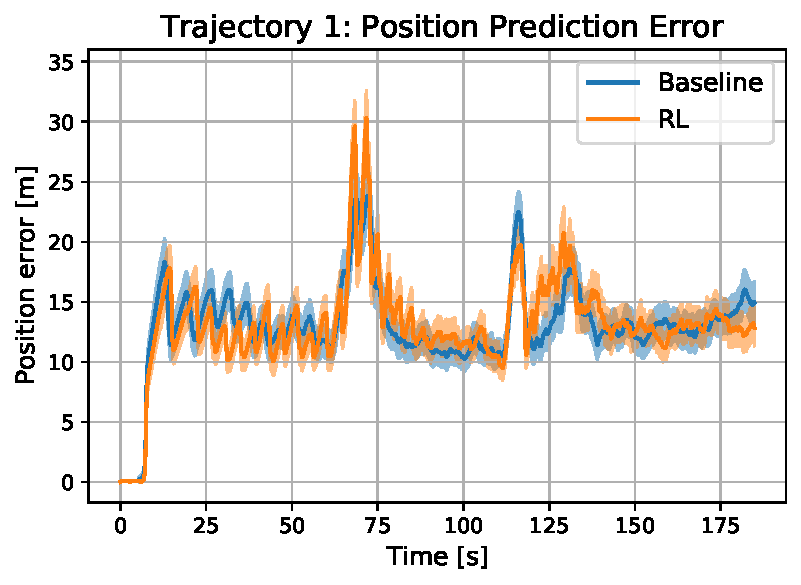
\includegraphics[width=\linewidth]{figures/benchmark/Simulations/mean_position_error0.pdf}
        \caption{Trajectory 1.}
        \label{fig:PE_T1}
    \end{subfigure}
    \hfill
    \begin{subfigure}[b]{0.45\textwidth}
        \centering
        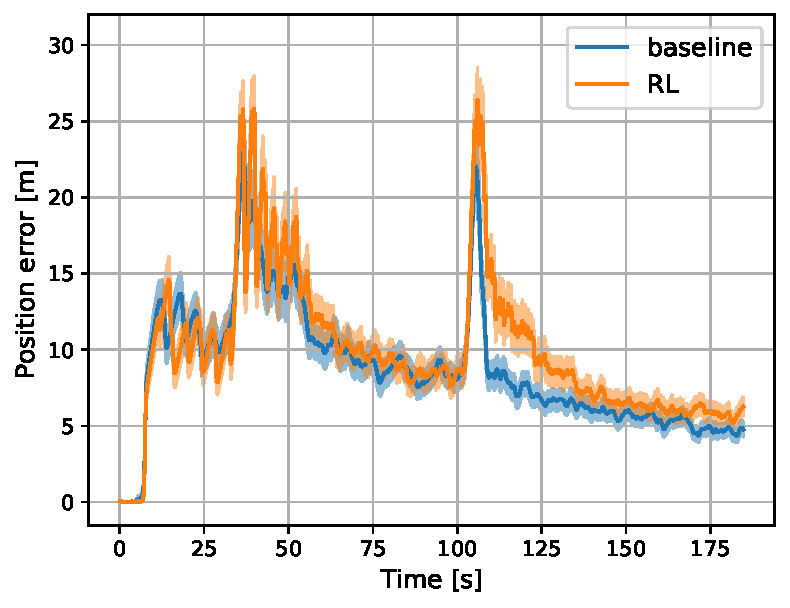
\includegraphics[width=\linewidth]{figures/benchmark/Simulations/mean_position_error1.pdf}
        \caption{Trajectory 2.}
        \label{fig:PE_T2}
    \end{subfigure}
    \hfill
    \begin{subfigure}[b]{0.45\textwidth}
        \centering
        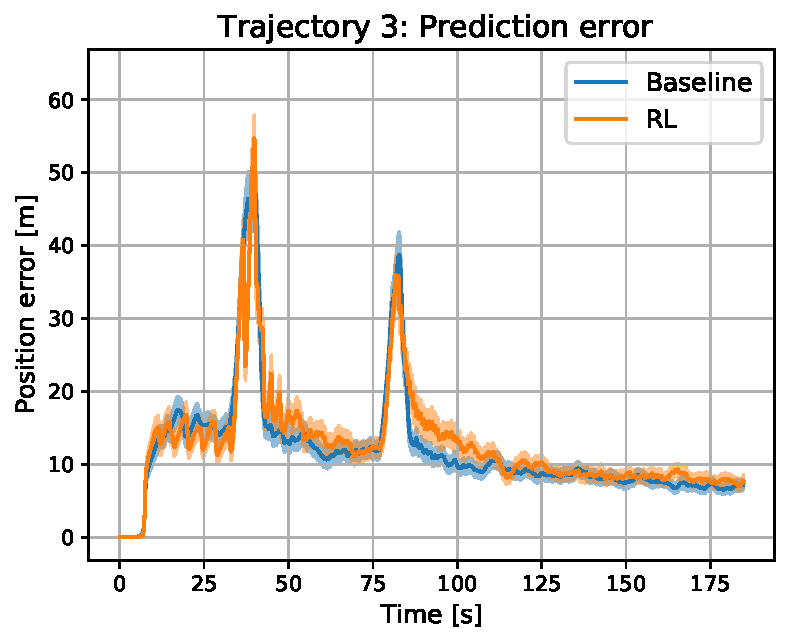
\includegraphics[width=\linewidth]{figures/benchmark/Simulations/mean_position_error2.pdf}
        \caption{Trajectory 3.}
        \label{fig:PE_T3}
    \end{subfigure}
    \hfill
    \begin{subfigure}[b]{0.45\textwidth}
        \centering
        \includegraphics[width=\linewidth]{figures/benchmark/Simulations/mean_position_error3.pdf}
        \caption{Trajectory 4.}
        \label{fig:PE_T4}
    \end{subfigure}
    \hfill
    \begin{subfigure}[b]{0.45\textwidth}
        \centering
        \includegraphics[width=\linewidth]{figures/benchmark/Simulations/mean_position_error4.pdf}
        \caption{Trajectory 5.}
        \label{fig:PE_T5}
    \end{subfigure}
    \hfill
    \begin{subfigure}[b]{0.45\textwidth}
        \centering
        \includegraphics[width=\linewidth]{figures/benchmark/Simulations/mean_position_error5.pdf}
        \caption{Trajectory 6.}
        \label{fig:PE_T6}
    \end{subfigure}
    \caption{Comparing the proposed reinforcement learning approach to the baseline algorithm in terms of error in predictive target position estimates.
    The figures provide expected revisit interval with 95\% confidence intervals.}
    \label{fig:position_error_comparison}
\end{figure}


\subsection{Summary}

The RIS problem was formulated as an RL problem by identifying suitable states, actions, and rewards, when assuming the monostatic radar described in Section \ref{sec:system_description}.
Mode probabilities of the IMM estimator, the most recent RIs, and innovations were discretized such that those could be used as states for the Q-learning algorithm.
Two different action spaces were identified, which are referred to as direct selection and delta selection.
The immediate rewards were proposed to balance the risk of losing a track and minimizing the tracking load.  

The most efficient state space was identified by simulating multiple differently configured  RL agents in the benchmark trajectories.
The agents using the mode probabilities had excellent performance in terms of the mean tracking load and the mean PLT.
The difference between the myopic and the non-myopic agents was also investigated.
The myopic agents learned faster and had better mean tracking load performance.
However, the non-myopic agents' ability to consider the long-term consequences resulted in lower PLT. 
Lastly, it was identified that augmenting the state presentations with the most recent RI does not significantly improve the tracking load performance.
Moreover, the larger state space leads to slower learning speed that causes higher PLT.  

The myopic RL agent using the mode probabilities as states was compared against the baseline algorithm in terms of the tracking load, the PLT, and the position prediction error.
It was found that the performance of the RL agent is comparable to the baseline algorithm.
The proposed learning-based approach can benefit from utilizing the experience to reduce the tracking load peaks compared to the baseline algorithm.
Future research directions could include function approximation techniques that could enable applying higher dimensional state spaces more efficiently. 
Furthermore, more efficient exploration strategies from the MAB framework could be investigated, especially when using the myopic policies.


\clearpage
\section{Conclusions} \label{sec:conclusions}


Radar Resource Management (RRM) algorithms are required for allocating and scheduling radar resources as well as to optimize the operational parameters of radars.  
Phased-array antenna technology, Multiple-Input Multiple-Output (MIMO) systems, and cognitive radars have increased the demand for intelligent RRM algorithms.
The RRM can be approached by dividing the RRM problem into subproblems that consider specific fields of RRM.
In this thesis, Reinforcement Learning (RL) methods were proposed for two specific RRM problems.
RL enables the radar systems to learn in real-time from experience without using any model developed beforehand.
In both RRM problems, RL methods were successfully applied to learn to act in the problems at hand. 
Furthermore, with a sufficient amount of learning, an advantage can be seen compared to the baseline algorithms.

In distributed MIMO radars, transmitter (TX) and receiver (RX) subsets are selected to reduce the power consumption and the data to be processed at the central processor as well as to prevent exposing the locations of the TXs for an adversary.
The Multi-Armed Bandit (MAB) framework was used to formulate the TX-RX selection problem as an RL problem.
Furthermore, the problem was modeled as a combinatorial MAB problem used to reduce the dimensions of the action space.
A MAB algorithm was proposed to actively learn to select a subset of TXs and RXs that maximize the reward function.

Each arm in the MAB formulation was modeled as a single TX-RX pair such that the RL agent selects multiple arms at a time. 
The exploration-exploitation trade-off ensured that all the different TX-RX pairs were probed for a sufficient number of times to minimize the regret. 
The RL agent's selections were driven by a reward function that calculates mean SINR in a linear scale.
A constant learning rate was used to weight past rewards less than recent rewards to address the time-dependent reward distributions for moving target scenarios.

The performance of the generalized MAB algorithm was evaluated in Monte Carlo simulations.
The simulation results exhibited that when using the RL approach, the mean SINR was close to optimal even in non-stationary scenarios and outperformed the exploration-free method.
However, the RL approach's limitation is that the radar was assumed to probe different subsets with short intervals.
Contextual multi-armed bandits \cite{Lu2010} could be used to address the non-stationary reward distributions and enable using the RL approach even with longer intervals. 

Adaptive Revisit Interval Selection (RIS) algorithms are used for decreasing the time budget allocated for tracking tasks.
RIS problem was addressed using the Q-learning algorithm meaning that the states, the actions, and the rewards were defined. 
Alternative state spaces were identified based on the innovation sequence, the mode probabilities of an IMM estimator, and the most recent revisit interval.
The proposed rewards quantify the cost of losing a track while emphasizing the agent for minimizing the tracking load.

Multiple RL agents with different configurations were simulated to identify the effective state space in terms of learning speed and performance.
In addition, myopic and non-myopic agents were evaluated to determine if the myopic policy is sufficient for the RIS problem.
The learning speed was significantly decreased when increasing the number of states.
Therefore, using only the mode probabilities as the states were identified to enable fast learning, low PLT, and low tracking load.
Furthermore, it was identified that the myopic policies achieve low tracking load with desirable PLT, and non-myopic agents obtain lower PLT, but the tracking load is considerably higher.
The myopic RL agent using the mode probabilities as states was compared against the baseline algorithm in terms of the tracking load, and the position prediction error.
The RL agent achieved lower tracking load peaks, which is essential when working on overload situations.
At the same time, the position prediction error was not significantly increased.

The RL approach for RIS could be improved in several different ways.
Notably, the learning speed was the subject of concern when using multiple features to present the discrete state.
The learning speed could be improved by applying function approximators \cite{Sutton2018} to generalize states-action pairs the agent has not seen before.  
Additionally, it would be possible to utilize more effective policies to handle the exploration-exploitation trade-off, especially in the myopic case.
In future research, RIS could also be extended by applying RL to control the dwell times.

Both of the RL approaches for the RRM problems were evaluated in the single target tracking scenario, such that the RL formulations and the simulations were less complicated. 
In future research, also the multi-target tracking scenario should be considered. 
It would require taking into account the low-level scheduling and the track association. 

\newpage
\thesisbibliography

\printbibliography


\end{document}
